%
% bgteubner class bundle
%
% bgteubner.tex
% Copyright 2003--2012 Harald Harders
%
% This program may be distributed and/or modified under the
% conditions of the LaTeX Project Public License, either version 1.3
% of this license or (at your opinion) any later version.
% The latest version of this license is in
%    http://www.latex-project.org/lppl.txt
% and version 1.3 or later is part of all distributions of LaTeX
% version 1999/12/01 or later.
%
% This program consists of all files listed in manifest.txt.
% ===================================================================
%\newif\iffuerentwickler
%\fuerentwicklertrue
% ===================================================================
%\PassOptionsToPackage{draft}{graphicx}
% ===================================================================
%\PassOptionsToClass{layoutraster}{bgteubner}
%\PassOptionsToClass{draft}{bgteubner}
%\PassOptionsToClass{headingoutside}{bgteubner}
%\PassOptionsToClass{tocleft}{bgteubner}
%\PassOptionsToClass{a5paper}{bgteubner}
%\PassOptionsToClass{boldvec}{bgteubner}
\PassOptionsToClass{titlepage}{bgteubner}
\PassOptionsToClass{ulinevec}{bgteubner}
%\PassOptionsToClass{exercisetotoc}{bgteubner}
%\PassOptionsToClass{smalltheorem}{bgteubner}
\documentclass[english,ngerman,greybox]{bgteubner}
% ===================================================================
\listfiles
\makeindex
% ===================================================================
% Einstellung des passenden Zeichensatzes
% F�r Windows:
%\usepackage[ansinew]{inputenc}
% F�r Unix und Linux
\usepackage[latin1]{inputenc}
% ===================================================================
% Wenn Sie im Ausdruck sehen wollen, wie das Dokument auf dem Papier
% im Zielformat aussieht, aktivieren Sie eine der beiden folgenden
% M�glichkeiten:
%\usepackage[frame]{crop}
%\usepackage[cam,a4,center]{crop}
% ===================================================================
%\usepackage[activate]{pdfcprot}
\usepackage{verbatim}
\usepackage{url}
\usepackage{printlen}[2001/12/09]
\usepackage[gen]{eurosym}
\usepackage[nice]{nicefrac}
\usepackage{float}
% ===================================================================
\usepackage[draft,margin]{hhfixme}
% ===================================================================
% !TEX root = main.tex
% !TEX encoding = Windows Latin 1
% !TEX TS-program = pdflatex
% 
% Archivo de particion de palabras

\hyphenation{%
  % Introduzca aqui las palabras que requieran division especial, separadas por espacios.
  % No se pueden usar acentos en estas palabras (a menos que se use codificacion UTF8).
  pa-la-bra guio-nes
  }


\endinput 
% ===================================================================
\newcommand*\feinschliff[4]{%
  \ifafive{\iftimes{#3}{#4}}{\iftimes{#1}{#2}}%
}
% ===================================================================
\let\np=\numprint
\def\ch#1{\ensuremath{\mathrm{#1}}}
\newcommand\TeXLive{\TeX Live}
\begingroup
\shorthandon{"}
\gdef\pdfLaTeX{\textsc{pdf}"-\LaTeX}
\endgroup
\DeclareRobustCommand\BibTeX{\textsc{Bib}\TeX}
% ===================================================================
\feinschliff{%
  \addtocontents{toc}{\protect\enlargethispage{-2\protect\baselineskip}}%
}{%
  \addtocontents{toc}{\protect\enlargethispage{-2\protect\baselineskip}}%
}{}{}
% ===================================================================
\uselengthunit{mm}
% ===================================================================
\makeatletter
\newcommand\cmoldstylenums[1]{%
  \ifhhcls@times
    \begingroup
      \spaceskip\fontdimen\tw@\font
      \usefont{OML}{\rmdefault}{\f@series}{it}%
      \mathgroup\symletters #1%
    \endgroup
  \else
    \oldstylenums{#1}%
  \fi
}
\newcommand\cmnewstylenums[1]{%
  \ifhhcls@times
    \begingroup
      \spaceskip\fontdimen\tw@\font
      \renewcommand\rmdefault{cmr}%
      \usefont{T1}{\rmdefault}{\f@series}{n}%
      \mathgroup\symletters #1%
    \endgroup
  \else
    \newstylenums{#1}%
  \fi
}
\makeatother
% ===================================================================
\makeatletter
\newcommand*\bsptheindex{%
  \renewenvironment{theindex}
  {\if@twocolumn
      \@restonecolfalse
    \else
      \@restonecoltrue
    \fi
    \columnseprule \z@
    \columnsep 20\p@
    \parindent\z@
    \setlength{\parskip}{\z@ \@plus .3\p@}%
    \setlength{\parfillskip}{\z@ \@plus 1fil}%
    \let\item\@idxitem
    \setlength\RaggedRightRightskip{\z@\@plus 4em}%
    \RaggedRight\listsfont}
  {}%
  \noindent
}
\makeatother
% ===================================================================
\newcommand\texindex[1]{\index{#1|emph}}
\newcommand\macroindex[1]{\index{#1@\texttt{\textbackslash #1}|emph}}
\newcommand\envindex[1]{\index{#1@\texttt{#1}"=Umgebung|emph}}
\newcommand\srcindex[1]{\index{#1@\texttt{#1}|emph}}
\newcommand\styindex[1]{\index{#1@\texttt{#1}"=Paket|emph}}
\newcommand\clsindex[1]{\index{#1@\texttt{#1}"=Klasse|emph}}
\newcommand\optindex[1]{\index{#1@\texttt{#1}"=Klassenoption|emph}}
% ===================================================================
\setindexpreamble{%
  \begingroup
  \setlength{\parindent}{\baselineskip}%
  \noindent\small
  Normalerweise sind Seitenzahlen aufrecht gedruckt.
  Wichtige Verweise, z.\,B.\ auf den Ort, an dem ein Begriff definiert
  wird, werden fett gedruckt, falls mehrere Seitenzahlen f�r diesen
  Begriff existieren.
  Seitenzahlen, die sich auf die Durchf�hrung mit \LaTeX\ beziehen,
  sind kursiv gedruckt.

  Da der finanzielle Rahmen f�r die Erstellung der Dokumentklasse
  sowie der Dokumentation begrenzt waren, habe ich mehr Wert darauf
  gelegt, dass die Klasse und die Dokumentation selbst vern�nftig
  getestet wurden, als dass das Stichwortverzeichnis vollst�ndig ist.
  Das Stichwortverzeichnis ist somit leider nur unvollst�ndig.
  Nehmen Sie das bitte nicht als Vorbild f�r Ihr Stichwortverzeichnis.
  \par
  \endgroup
  \bigskip
}
% ===================================================================
%\version{1.10}
% ===================================================================
\makeglossary[cmd]
\newcommand*\glossarycmdname{}
\addto\captionsgerman{\renewcommand*\glossarycmdname{Befehlsreferenz}}
\addto\captionsngerman{\renewcommand*\glossarycmdname{Befehlsreferenz}}
\addto\captionsaustrian{\renewcommand*\glossarycmdname{Befehlsreferenz}}
\addto\captionsnaustrian{\renewcommand*\glossarycmdname{Befehlsreferenz}}
\addto\captionsenglish{\renewcommand*\glossarycmdname{Command reference}}
\renewcommand\glossarycmdpreamble{%
  \addchap{\glossarycmdname}%
  \label{sec:befehlsreferenz}%
  In dieser Befehlsreferenz sind haupts�chlich die Befehle und
  Umgebungen aufgef�hrt, die von der
  \texttt{bgteubner}-Klasse zus�tzlich zum Standard bzw.\ der Klasse
  \texttt{scrbook} aus dem \acro{KOMA}-Script-Paket definiert
  werden.
  
  In Klammern wird jeweils der Abschnitt angegeben, in dem n�here
  Erkl�rungen gefunden werden k�nnen.
}
% ===================================================================
\floatstyle{komabelow}
\newfloat{graphics}{tp}{gra}[chapter]
\floatname{graphics}{Grafik}
% ===================================================================
\makeatletter
\def\makeactive#1{\catcode`#1=13 }
\def\makeescape#1{\catcode`#1=\z@}
\def\makebgroup#1{\catcode`#1=\@ne}
\def\makeegroup#1{\catcode`#1=\tw@}
\let\@TBverbatim\verbatim
\let\@TBendverbatim\endverbatim
\def\verbatim{\obeylines
  \futurelet\reserved@a\@switch@sqbverbatim}
\def\@switch@sqbverbatim{\ifx\reserved@a[%]
  \expandafter\@sqbverbatim\else
  \def\reserved@b{\@sqbverbatim[]}\expandafter\reserved@b\fi}
\def\@sqbverbatim[#1]{%
  \par
  \def\ruled{\let\if@ruled\iftrue}%
  #1\@TBverbatim}
\let\if@ruled\iffalse
\def\@verbatim{%
    \if@ruled\trivlist\item\hrule\kern5\p@\nobreak\fi
  \trivlist \item\relax
  \if@minipage\else\vskip\parskip\fi
  \leftskip\@totalleftmargin\rightskip\z@skip
  \parindent\z@\parfillskip\@flushglue\parskip\z@skip
  \@@par
  \@tempswafalse
  \def\par{%
    \if@tempswa
      \leavevmode \null \@@par\penalty\interlinepenalty
    \else
      \@tempswatrue
      \ifhmode\@@par\penalty\interlinepenalty\fi
    \fi}%
  \obeylines \verbatim@font \@noligs
  \let\do\@makeother \dospecials
  \everypar \expandafter{\the\everypar \unpenalty}%
}%
\def\endverbatim{\@TBendverbatim
  \if@ruled\kern5\p@\hrule\endtrivlist\fi}
{\makeactive<
  \gdef<#1>{{\reset@font\ensuremath{\langle}%
    \textit{#1}%
    \ensuremath{\rangle}}}
}
\makeatother
% =====================================================================
\makeatletter
\DeclareRobustCommand\meta[1]{%
     \ensuremath\langle
     \ifmmode \expandafter \nfss@text \fi
     {%
      \meta@font@select
      \edef\meta@hyphen@restore
        {\hyphenchar\the\font\the\hyphenchar\font}%
      \hyphenchar\font\m@ne
      \language\l@nohyphenation
      #1\/%
      \meta@hyphen@restore
     }\ensuremath\rangle
}
\def\meta@font@select{\normalfont\itshape}
\DeclareRobustCommand\cs[1]{\texttt{\char`\\#1}}
\DeclareRobustCommand\env[1]{\texttt{#1}}
\providecommand\marg[1]{%
  {\ttfamily\char`\{}\meta{#1}{\ttfamily\char`\}}}
\providecommand\oarg[1]{%
  {\ttfamily[}\meta{#1}{\ttfamily]}}
\providecommand\parg[1]{%
  {\ttfamily(}\meta{#1}{\ttfamily)}}
\makeatother
% ===================================================================
\begingroup
\makeatletter
\fixme@marginfalse
\makeatother
\fixme{Index vervollst�ndigen}%
\fixme{Hinweis auf kleine Unterschiede zwischen cm und Times}%
\endgroup
%\AtEndDocument{\listoffixmes}%
% ===================================================================
\begin{document}
% ===================================================================
\frontmatter
% ===================================================================
% Titel des Buches:
\GetFileInfo{bgteubner.cls}
\title{Erstellen von B�chern f�r den Springer Vieweg Verlag mit \LaTeX}
% Untertitel:
\subtitle{Autorenrichtlinien und Installationsanleitung f�r Version
  \fileversion\ der Dokumentklasse}
% Angabe der Autoren
% Optionales Argument: Autorenname mit Titel
% 1. Hauptargument: Autorenname, nur Vor- und Nachname
% 2. Hauptargument: Institutsname dieses Autoren
\author{Harald Harders}
% Auflagennummer:
%\edition{Vorabversion vom 04.\,09.~2003}
%\edition{1}
% ===================================================================
% Titelseite erzeugen
\maketitle
% Titel nochmal eingeben, aber ohne Befehl, weil \pdfinfo damit nicht
% klarkommt.
\title{Erstellen von B�chern f�r den Springer Vieweg Verlag mit LaTeX}%
% ===================================================================
\chapter{Vorwort} 	% engl. Preface


Dies ist \textbf{Version \hgbDate} der \latex-Dokumentenvorlage für 
verschiedene Abschlussarbeiten an der Fakultät für Informatik, Kommunikation
und Medien der FH Oberösterreich in Hagenberg, die mittlerweile auch 
an anderen Hochschulen im In- und Ausland gerne verwendet wird.

Das Dokument entstand ursprünglich auf Anfragen von Studierenden,
nachdem im Studienjahr 2000/01 erstmals ein offizieller
\latex-Grundkurs im Studiengang Medientechnik und -design an der
FH Hagenberg angeboten wurde. Eigentlich war die Idee, die bereits
bestehende \emph{Word}-Vorlage für Diplomarbeiten "einfach" in
\latex\ zu übersetzen und dazu eventuell einige spezielle
Ergänzungen einzubauen. Das erwies sich rasch als wenig
zielführend, da \latex, \va was den Umgang mit Literatur und
Grafiken anbelangt, doch eine wesentlich andere Arbeitsweise
verlangt. Das Ergebnis ist -- von Grund auf neu geschrieben und
wesentlich umfangreicher als das vorherige Dokument --
letztendlich eine Anleitung für das Schreiben mit \latex, ergänzt
mit einigen speziellen (mittlerweile entfernten) Hinweisen für \emph{Word}-Benutzer.
Technische Details zur aktuellen Version finden sich in Anhang \ref{app:TechnischeInfos}.

Während dieses Dokument anfangs ausschließlich für die Erstellung
von Diplomarbeiten gedacht war, sind nunmehr auch  
\emph{Masterarbeiten}, \emph{Bachelor\-arbeiten} und \emph{Praktikumsberichte} 
abgedeckt, wobei die Unterschiede bewusst gering gehalten wurden.

Bei der Zusammenstellung dieser Vorlage wurde versucht, mit der
Basisfunktionalität von \latex das Auslangen zu finden und -- soweit möglich --
auf zusätzliche Pakete zu verzichten. Das ist nur zum Teil gelungen;
tat\-säch\-lich ist eine Reihe von ergänzenden "Paketen" notwendig, wobei jedoch
nur auf gängige Erweiterungen zurückgegriffen wurde.
Selbstverständlich gibt es darüber hinaus eine Vielzahl weiterer Pakete,
die für weitere Verbesserungen und Finessen nützlich sein können. Damit kann
sich aber jeder selbst beschäftigen, sobald das notwendige Selbstvertrauen und
genügend Zeit zum Experimentieren vorhanden sind.
Eine Vielzahl von Details und Tricks sind zwar in diesem Dokument nicht explizit
angeführt, können aber im zugehörigen Quelltext jederzeit ausgeforscht
werden.

Zahlreiche KollegInnen haben durch sorgfältiges Korrekturlesen und
konstruktive Verbesserungsvorschläge wertvolle Unterstützung
geliefert. Speziell bedanken möchte ich mich bei Heinz Dobler für
die konsequente Verbesserung meines "Computer Slangs", bei
Elisabeth Mitterbauer für das bewährte orthographische Auge und
bei Wolfgang Hochleitner für die Tests unter Mac~OS.

Die Verwendung dieser Vorlage ist jedermann freigestellt und an
keinerlei Erwähnung gebunden. Allerdings -- wer sie als Grundlage
seiner eigenen Arbeit verwenden möchte, sollte nicht einfach
("ung'schaut") darauf los werken, sondern zumindest die
wichtigsten Teile des Dokuments \emph{lesen} und nach Möglichkeit
auch beherzigen. Die Erfahrung zeigt, dass dies die Qualität der
Ergebnisse deutlich zu steigern vermag.

Dieses Dokument und die zugehörigen \latex-Klassen sind seit Nov.\ 2017 auf CTAN%
\footnote{Comprehensive TeX Archive Network} 
als Paket \texttt{hagenberg-thesis} verfügbar unter
%
\begin{itemize}
\item[]\url{https://ctan.org/pkg/hagenberg-thesis}.
\end{itemize}
%
Den jeweils aktuellen Quelltexte sowie zusätzliche Materialien findet man unter
%
\begin{itemize}
\item[]\url{https://github.com/Digital-Media/HagenbergThesis}.%
\footnote{Unter \url{https://github.com/Digital-Media/HagenbergThesis/blob/master/CHANGELOG.md}
sowie genauer unter \url{https://github.com/Digital-Media/HagenbergThesis/commits/master} 
findet man auch eine (früher im Anhang dieses Dokuments enthaltene) chronologische Auflistung der 
Änderungen.}
\end{itemize}



\noindent
Trotz großer Mühe enthält ein Dokument wie dieses immer Fehler und Unzulänglichkeiten
-- Kommentare, Verbesserungsvorschläge und sinnvolle Ergänzungen
sind daher willkommen, am einfachsten als Kommentar oder Fehlermeldung ("Issue") 
auf GitHub oder jederzeit auch per E-Mail an
%
\begin{itemize}
\item[]
Dr.\ Wilhelm Burger, Department für Digitale Medien,\newline
Fachhochschule Oberösterreich, Campus Hagenberg (Österreich)\newline
\nolinkurl{wilhelm.burger@fh-hagenberg.at}
\end{itemize}

\noindent
Übrigens, hier im Vorwort (das bei Diplom- und Masterarbeiten üblich, bei Bachelorarbeiten 
aber entbehrlich ist) kann kurz auf die Entstehung des Dokuments eingegangen werden.
Hier ist auch der Platz für allfällige Danksagungen (\zB an den Betreuer, 
den Begutachter, die Familie, den Hund, \ldots), Widmungen und philosophische 
Anmerkungen. Das sollte man allerdings auch nicht übertreiben und auf 
einen Umfang von maximal zwei Seiten beschränken.





\tableofcontents
\mainmatter
% ===================================================================

\chapter{Einleitung}
\label{cha:Einleitung}

\section{Zielsetzung}
Dieses Dokument ist als vorwiegend technische Starthilfe für das
Erstellen einer Masterarbeit (oder Bachelorarbeit) mit \latex
gedacht und ist die Weiterentwicklung einer früheren
Vorlage\footnote{Nicht mehr verfügbar.} für das Arbeiten mit
Microsoft \emph{Word}. Während ursprünglich daran gedacht war, die
bestehende Vorlage einfach in \latex zu übernehmen, wurde rasch
klar, dass allein aufgrund der großen Unterschiede zum Arbeiten
mit \emph{Word} ein gänzlich anderer Ansatz notwendig wurde. Dazu
kamen zahlreiche Erfahrungen mit Diplomarbeiten in den
nachfolgenden Jahren, die zu einigen zusätzlichen Hinweisen Anlass gaben.

Das vorliegende Dokument dient einem zweifachen Zweck: 
\emph{erstens} als Erläuterung und Anleitung, \emph{zweitens} als
direkter Ausgangspunkt für die eigene Arbeit. Angenommen wird,
dass der Leser bereits über elementare Kenntnisse im Umgang mit
\latex verfügt. In diesem Fall sollte -- eine einwandfreie
Installation der Software vorausgesetzt -- der Arbeit nichts mehr
im Wege stehen. Auch sonst ist der Start mit \latex\ nicht
schwierig, da viele hilfreiche Informationen auf den zugehörigen
Webseiten zu finden sind (s.\ Kap.~\ref{cha:ArbeitenMitLatex}).





\section{Warum {\latex}?}

Diplomarbeiten, Dissertationen und Bücher im
technisch-natur\-wissen\-schaft\-lichen Bereich werden
traditionell mithilfe des Textverarbeitungssystems \latex
\cite{Lamport1994, Lamport1995} gesetzt. Das hat gute Gründe, denn
\latex ist bzgl.\ der Qualität des Druckbilds, des Umgangs mit
mathematischen Elementen, Literaturverzeichnissen etc.\
unübertroffen und ist noch dazu frei verfügbar. Wer mit \latex
bereits vertraut ist, sollte es auch für die Abschlussarbeit
unbedingt in Betracht ziehen, aber auch für den Anfänger sollte
sich die zusätzliche Mühe am Ende durchaus lohnen.

Für den professionellen elektronischen Buchsatz wurde früher
häufig \emph{Adobe Framemaker} verwendet, allerdings ist diese
Software teuer und komplex. Eine modernere Alternative dazu ist
\emph{Adobe InDesign}, wobei allerdings die Erstellung
mathematischer Elemente und die Verwaltung von Literaturverweisen
zur Zeit nur rudimentär unterstützt werden.%
\footnote{Angeblich werden aber für den (sehr sauberen) Schriftsatz 
in \emph{InDesign} ähnliche Algorithmen wie in \latex\ verwendet.}

Microsoft \emph{Word} gilt im Unterschied zu \latex, 
\emph{Framemaker} und \emph{InDesign} übrigens nicht als professionelle
Textverarbeitungssoftware, obwohl es immer häufiger auch von
großen Verlagen verwendet wird.%
\footnote{Siehe auch \url{http://latex.tugraz.at/mythen.php}.}
Das Schriftbild in \emph{Word}
lässt -- zumindest für das geschulte Auge -- einiges zu wünschen
übrig und das Erstellen von Büchern und ähnlich großen Dokumenten
wird nur unzureichend unterstützt. Allerdings ist \emph{Word} sehr
verbreitet, flexibel und vielen Benutzern zumindest oberflächlich
vertraut, sodass das Erlernen eines speziellen Werkzeugs wie
\latex\ ausschließlich für das Erstellen einer Abschlussarbeit
manchen verständlicherweise zu mühevoll ist. Es sollte daher
niemandem übel genommen werden, wenn er/sie sich auch bei der Abschlussarbeit
auf \emph{Word} verlässt. Im Endeffekt lässt sich mit etwas
Sorgfalt (und ein paar Tricks) auch damit ein durchaus akzeptables
Ergebnis erzielen. 
Ansonsten sollten auch für \emph{Word}-Benutzer 
einige Teile dieses Dokuments von Interesse sein, insbesondere die
Abschnitte über Abbildungen und Tabellen
(Kap.~\ref{cha:Abbildungen}) und mathematische Elemente
(Kap.~\ref{cha:Mathematik}).


\section{Aufbau der Arbeit}

Hier am Ende des Einleitungskapitels (und nicht
etwa in der Kurzfassung) ist der richtige Platz, um die
inhaltliche Gliederung der nachfolgenden Arbeit zu beschreiben.
Hier sollte man darstellen, welche Teile (Kapitel) der Arbeit
welche Funktion haben und wie sie inhaltlich zusammenhängen. Auch
die Inhalte des \emph{Anhangs} -- sofern vorgesehen -- sollten hier
kurz beschrieben werden.

Zunächst sind in Kapitel \ref{cha:Abschlussarbeit} einige wichtige
Punkte zu Abschlussarbeiten im Allgemeinen zusammengefasst.
Kapitel \ref{cha:ArbeitenMitLatex} beschreibt die Idee und die
grundlegenden technischen Eigenschaften von \latex.
Kapitel \ref{cha:Abbildungen} widmet sich der Erstellung von Abbildungen
und Tabellen sowie der Einbindung von Quellcode.
Mathematische Elemente und Gleichungen sind das Thema in Kapitel \ref{cha:Mathematik} 
\usw
Anhang \ref{app:TechnischeInfos} enthält technische Details zu
dieser Vorlage, 
Anhang \ref{app:cdrom} enthält eine Auflistung von zugehörigen Materialien
auf einem beigelegten Speichermedium, und 
Anhang \ref{app:Fragebogen} zeigt ein Beispiel für die
Einbindung eines mehrseitigen PDF-Dokuments.








\addpart{Typographie\label{part:allgemeines}}%
%
% bgteubner class bundle
%
% globales.tex
% Copyright 2003--2012 Harald Harders
%
% This program may be distributed and/or modified under the
% conditions of the LaTeX Project Public License, either version 1.3
% of this license or (at your opinion) any later version.
% The latest version of this license is in
%    http://www.latex-project.org/lppl.txt
% and version 1.3 or later is part of all distributions of LaTeX
% version 1999/12/01 or later.
%
% This program consists of all files listed in manifest.txt.
% ===================================================================
\chapter{Globales}%
\index{Globales}%

% ===================================================================
\section{Gesamtaufbau}%
\label{sec:gesamtaufbau}%
\index{Gesamtaufbau}%
\index{Aufbau}%

Das Innere eines Buchs aus dem Teubner Verlag beginnt mit dem
\index{Schmutztitel}\new{Schmutztitel,} auf dem nur die Autoren und
der Buchtitel abgedruckt sind.
Auf dieser Seite beginnt die, im \index{Titelei}Vorspann r�mische,
\index{Seitenz�hlung}Seitenz�hlung mit~\iftimes{I}{\textsc{i}}. 
Auf der n�chsten rechten Seite wird der
\index{Innentitel}\new{Innentitel,} auf dem alle wichtigen
Informationen (\index{Autor}Autoren, \index{Titel}Titel,
\index{Untertitel}Untertitel, \index{Auflage@Auf\/lage}Auf"|lage,
\index{Erscheinungsjahr}Erscheinungsjahr, \dots) enthalten sind, gesetzt.
Das \index{Impressum}\new{Impressum} befindet sich auf
Seite~\iftimes{IV}{\textsc{iv}}.
Um diese ersten Seiten des Buches brauchen Sie sich nicht zu k�mmern,
da diese vom Teubner Verlag separat erstellt werden.

Es folgt auf Seite~\iftimes{V}{\textsc{v}} das
\index{Vorwort}\new{Vorwort,} das normalerweise die �berschrift
"`Vorwort"' erh�lt. 
Daran angeschlossen wird das
\index{Inhaltsverzeichnis}\new{Inhaltsverzeichnis.}
Eventuelle \index{Formelverzeichnis}Formel"~,
\index{Abk�rzungsverzeichnis}Abk�rzungs"~,
\index{Abbildungsverzeichnis}Abbildungs"= und
\index{Tabellenverzeichnis}Tabellenverzeichnisse werden im Anhang
eingef�gt.
Sie werden \emph{nicht} vor den eigentlichen Inhalt des Buches
gesetzt.

Nun wird die \index{Seitenz�hlung}Seitenz�hlung bei~1 in arabischen
Zahlen neu begonnen.  
Diese Seitennummerierung wird f�r das restliche Buch beibehalten.
Auf Seite~1 beginnt das erste Kapitel des Buchs.
Der inhaltliche Anteil des Buches kann (muss aber nicht) in mehrere
\index{Teil}\new{Teile} eingeteilt werden, die jeweils durch eine
ungerade Seite, auf der nur der Name des Buchteils
geschrieben steht, begonnen werden.
Zum Beispiel stellt Seite~\pageref{part:allgemeines} dieser
Richtlinien eine solche Teil�berschrift dar.
Die einzelnen Teile k�nnen unnummeriert oder r�misch durchnummeriert
sein.

Die Kapitel und Abschnitte werden arabisch nach dem Muster
\index{Kapitel!nummerierung@"~nummerierung}1, 1.1, 1.1.1 nummeriert.

Es folgt ein \index{Anhang}\new{Anhang,} der immer ein unnummerierter
Teil, entsprechend dem eben beschriebenen, ist.
Dort wird die \index{Kapitel!nummerierung@"~nummerierung}Nummerierung
auf \iftimes{A}{\textsc{a}}, \iftimes{A.1}{\textsc{a}.1},
\iftimes{A.1.1}{\textsc{a}.1.1} umgestellt.
Der Anhang beginnt mit Kapiteln, die inhaltlichen Charakter haben,
beispielsweise weitergehenden Herleitungen, die aus dem eigentlichen
Inhalt des Buches herausfallen.

Die letzten Kapitel des Anhanges werden duch die Verzeichnisse
(\index{Literaturverzeichnis}Literaturverzeichnis,
\index{Formelzeichenverzeichnis}Formelzeichenverzeichnis,
\index{Stichwortverzeichnis}Stichwortverzeichnis, \ldots) gebildet.
Dabei d�rfen einzelne Verzeichnisse fortgelassen werden, sofern sie
dem Autoren unn�tig erscheinen.
Allerdings sind das Literatur"= und das Stichwortverzeichnis
obligatorisch. 


% ===================================================================
\section{Seitenformat und "~aufteilung}%
\label{sec:seitenformat}%
\index{Seitenformat}%
\index{Seitenaufteilung}%
\index{Satzspiegel}%

F�r B�cher des Teubner Verlags stehen zwei
\index{Format}\index{Papierformat}Formate zur Auswahl:
\acro{DIN"~A\,5} ($\np[mm]{148}\times\np[mm]{210}$) und
$\np[mm]{170}\times\np[mm]{240}$.
Die Satzspiegel wurden mit
$\np[mm]{115}\times\np[mm]{174}$ bzw.\
$\np[mm]{135}\times\np[mm]{200}$ inklusive Kolumnentitel vom Verlag
vorgegeben.

Der �u�ere \index{Rand}Rand auf jeder Seite soll optisch genauso breit
sein wie beide R�nder in der Buchmitte zusammen \cite{kohm2003a}.
Damit dies erreicht wird, ist mittlere Rand auf einem vollst�ndig
sichtbarem Blatt (z.\,B.\ einem Probeausdruck) etwas breiter als der
halbe �u�ere Rand, da in der Mitte etwas Fl�che durch die Bindung
verloren geht.


% ===================================================================
\section{Schriften}%
\label{sec:schrift}%
\index{Schrift}%

Auch f�r die \index{Brotschrift}\new{Brotschrift} sind zwei Varianten
m�glich.
Normalerweise wird die \index{Times Roman}%
\iftimes{"`Times Roman"'}{{\usefont{T1}{ptm}{m}{n}"`Times Roman"'}}
verwendet, die der Windows"=Standardschrift Times""New""Roman sehr
�hnlich ist und daher ein einheitliches Aussehen von B�chern
erm�glicht, die mit \LaTeX\ oder mit Microsoft Word erstellt
wurden.\iftimes{\footnote{Das ist bei diesem Dokument der Fall.}}{} 
Mit ihr wird gegebenenfalls als serifenlose die \index{Helvetica}%
\iftimes{\textsf{"`Helvetica"'}}{{\usefont{T1}{phv}{m}{n}"`Helvetica"'}}
und als Schreibmaschinenschrift die \index{Courier}%
\iftimes{\texttt{"`Courier"'}}{{\usefont{T1}{pcr}{m}{n}"`Courier"'}}
kombiniert.

Nach Absprache mit dem zust�ndigen Lektor kann aber auch die
Schrift \index{European Computer Modern}%
\iftimes{{\usefont{T1}{cmr}{m}{n}"`European Computer
    Modern"'}}{"`European Computer Modern"'} Antiqua, die bei \LaTeX\
weit verbreitet ist, verwendet
werden.\iftimes{}{\footnote{Das ist bei diesem Dokument der Fall.}}
Sie bricht zwar die Einheitlichkeit im Aussehen der B�cher etwas auf,
bietet daf�r aber, gerade im mathematischen Satz, einige
Vorteile.\footnote{Sofern die kommerziellen Schriftpakete MathTime und
  MathTimePlus von der Firma Y\,\&\,Y verf�gbar sein sollten, kann
  durch sie der mathematische Schriftsatz auch mit der Times vern�ftig
  gestaltet werden (siehe dazu Tabelle~\ref{tab:klassenoptionen} auf
  Seite~\pageref{tab:klassenoptionen}.}
Sie wird mit ihrer 
\iftimes{{\usefont{T1}{cmss}{m}{n}serifenlosen}}{\textsf{serifenlosen}}
und 
\iftimes{{\usefont{T1}{cmtt}{m}{n}Schreibmaschinen}}%
{\texttt{Schreibmaschinen}}"=Variante kombiniert.

F�r beide Schriftfamilien gilt, dass f�r den Flie�text der
\index{Schriftgrad}%
\index{Punkt (Ma�einheit)}Schriftgrad 10~Punkt (abgek�rzt
$\np[pt]{10}$)\footnote{Die Einheit "`Punkt"' ist nicht eindeutig
  definiert.
  In \LaTeX\ hat $\np[pt]{1}$ die L�nge $\nicefrac{1}{72,27}$~inch.
  Ein Postscript"=Punkt hat die L�nge $\nicefrac{1}{72}$~inch und wird
  in \LaTeX\ mit $\np[bp]{1}$ bezeichnet (f�r \engl{big point}).
  Da der Unterschied so gering ist, dass er f�r Schriftgr��en
  unerheblich ist, gehe ich nicht weiter auf den Unterschied ein.}
verwendet wird.
Weitere verwendete \index{Schriftgrad}Schriftg��en sind f�r
Kapitel�berschriften 14,4 Punkt, f�r Abschnitts�berschriften 12~Punkt.
Einige Bereiche, wie z.\,B.\ Bildunterschriften, werden in einer
9"=Punkt"=Schrift gesetzt, Fu�noten in 8~Punkt.

Bei Verwendung der European"=Computer"=Modern"=Schriftfamilie werden
Zahlen im Text als
\index{Medi�valziffer}\new{Medi�valziffern}
(\cmoldstylenums{1234567890})%
\iftimes{\footnote{Die Zahlenbeispiele werden in der European Computer
    Modern gesetzt, da Medi�valziffern f�r die Times nicht zur
    Verf�gung stehen.}}{}
geschrieben, da diese weniger als die meist verwendeten
\index{Versalziffer}\new{Versalziffern}
(\cmnewstylenums{1234567890}) aus dem Flie�text herausstechen.
Beispielsweise sieht die Zahl \cmoldstylenums{1980} eher nach einem
normalen Wort mit Kleinbuchstaben aus als \cmnewstylenums{1980}, das
aussieht, als w�re es mit Versalien gedruckt.
Noch auf"|f�lliger ist es bei Telefonnummern.
Zum Beispiel f�llt (\cmoldstylenums{05\,31})
\cmoldstylenums{3\,91}"=\cmoldstylenums{30\,62} im Text weniger auf
und ist besser zu lesen als \cmnewstylenums{(05\,31) 3\,91"=30\,62}.
Wird die Times verwendet, m�ssen Versalziffern verwendet
werden, da f�r sie keine kostenlosen Medi�valziffern zur Verf�gung
stehen.

In mathematischem Formelsatz werden im Gegensatz zum Text immer
\index{Versalziffer}Versalziffern verwendet, um
Verwechslungen mit tiefgestellten Zeichen wie Indizes zu vermeiden.
Wegen dieser Unterscheidung ist es --~zumindest bei Verwendung der
European Computer Modern~-- sehr wichtig, beim Erstellen des
Dokumentes darauf zu achten, ob eine Zahl als Bestandteil des Textes
(z.\,B. Jahresangaben, Telefonnummern, Postleitzahlen) oder als
mathematische Formel gesehen werden soll.
Achten Sie bitte auch dann auf die Unterscheidung, wenn Sie die Times
verwenden.
Vielleicht soll ja sp�ter doch auf European Computer Modern umgestellt
werden.

\new{Hervorhebungen}\index{Hervorhebung} im Text werden durch
\emph{eine \index{kursiv}kursive Schrift} erzielt.
Verwenden Sie bitte keinen \index{fett}\textbf{Fettdruck,} da er beim blo�en
Anschauen der Seite sofort ins Auge springt.
Normalerweise ist das aber nicht gew�nscht. Stattdessen soll der Leser
lediglich beim normalen Lesen des Textes erkennen, dass dieses Wort
wichtig ist.
V�llig verboten sind mehrfache Auszeichnungen wie z.\,B.\
\emph{\bfseries fett und kursiv gleichzeitig.}
Es bietet sich an, neu eingef�hrte Begriffe beim ersten Auftreten
einmal kursiv zu drucken, wie es auch in den Autorenrichtlinien getan
wird.
F�hren Sie bitte neue Begriffe nicht mit
\index{Anf�hrungszeichen}Anf�hrungszeichen ein. 
Diese sollten nur dann verwendet werden, wenn wirklich auf einen
zitierten Titel verwiesen wird oder das Wort �hnlich w�rtlicher Rede
(z.\,B.\ sprichw�rtlich) verwendet wird.
\begin{example}
  Die Begriffe \new{Elastizit�tsmodul}, \new{Streckgrenze} und
  \new{Bruchdehnung} haben etwas mit Werkstoffkunde zu tun.

  Eine hydraulische Pr�fmaschine kann als wahre "`Kaputtmachmaschine"'
  angesehen werden.
\end{example}
Als \index{Anf�hrungszeichen|textbf}\new{Anf�hrungszeichen} werden
ausschlie�lich die nach innen zeigenden
\index{Guillemet}\new{Guillemets} (franz�sische Anf�hrungszeichen,
auch "`M�wchen"') "` und "' verwendet. 
Sowohl nach au�en zeigende Guillemets \flqq\dots\frqq, die deutschen
\quotedblbase\dots\textquotedblleft\ als auch englische
Anf�hrungsstriche (``\dots'') sind verboten.
F�r einfache Anf�hrungszeichen gilt das Gleiche: Es d�rfen nur \glq\
und \grq\ verwendet werden.
Dies ist folgenderma�en zu begr�nden (aus Friedrich Forssman, Ralf de
Jong: \emph{Detailtypografie}, S.~179~\cite{forssman2002a}):
\par
\begin{quote}
  Die \quotedblbase deutschen Anf�hrungen\textquotedblleft\ sind
  \emph{nicht so gut lesbar} [...] wie die "`M�wchen"',
  \begin{compactitem}
  \item denn sie gleichen den \emph{Apostrophen} und \emph{Kommas,}
  \item sie st�ren die \emph{Zeilenbildung} durch ihr aus der
    Zeilenmitte ger�cktes Bild.
  \end{compactitem}
  \feinschliff{\sloppypar}{}{}{}%
  Die \emph{franz�sischen Anf�hrungen} hingegen �hneln anderen
  Interpunktionszeichen nicht und unterst�tzen die
  Zeilenbildung.
\end{quote}
\par\noindent
Wenn Ihnen diese Anf�hrungszeichen ungewohnt erscheinen, schlagen Sie
einmal einige beliebige Romane auf.
Fast immer werden Guillemets verwendet.


% ===================================================================
\section{Abs�tze}%
\label{sec:allg_absaetze}%
\index{Absatz}%

Im Flie�text wird \index{Blocksatz}\new{Blocksatz} verwendet.
Die erste Zeile eines jeden Absatzes wird um den Betrag des
Zeilenabstandes
\index{Absatz!Einr�ckung}\index{Einr�ckung}einger�ckt.
Eine Ausnahme bildet der jeweils erste Absatz nach einer Kapitel"=
oder Abschnitts�berschrift, nach einem Abschnittswechsel ohne
�berschrift oder nach bestimmten, abgesetzt formatieren Bereichen, die
sp�ter beschrieben werden.
F�r die richtige Einr�ckung wird automatisch gesorgt.
Ein zus�tzlicher \index{Durchschuss}\new{Durchschuss} (gr��erer
Abstand) an Abs�tzen wird nicht vorgenommen.\footnote{Unter Umst�nden
  werden Abs�tze doch ein wenig auseinander gezogen, wenn dadurch
  verhindert werden kann, dass am unteren Rand des Satzspiegels L�cken
  entstehen.
  Dies ist unerw�nscht, vgl. Abschnitt~\ref{sec:tex_feinschliff}.}

Nach abgesetzten \index{mathematische Formel}mathematischen Formeln
\index{Mathematik}h�ngt es vom Kontext ab, ob
die folgende Zeile einger�ckt wird oder nicht.
Formeln gelten als ganz normale Satzteile. 
Geht nach ihnen der Satz oder der Gedankengang weiter, darf die
n�chste Zeile nicht einger�ckt werden.
F�ngt ein neuer inhaltlicher Punkt an, so muss die n�chste Zeile
einger�ckt werden.
Das l�sst sich an zwei einfachen Beispielen verdeutlichen.
\begin{example}
  \label{ex:absatz_bsp1}%
  Irgendwann vor unserer Zeit wurde der mathematische Satz des
  Pythagoras,
  \begin{align*}
    a^2+b^2 &= c^2\,,
  \end{align*}%
  entdeckt.
  Er besagt, dass die L�ngen eines rechtwinkligen Dreiecks 
  zueinander in Beziehung stehen.
\end{example}
Hier wird der Satz nach der Formel fortgef�hrt.
Es erfolgt keine Einr�ckung.
Im n�chsten Beispiel beginnt nach der Formel ein neuer Gedanke, der
durch einen neuen Absatz kenntlich gemacht wird.
\begin{example}
  \label{ex:absatz_bsp2}%
  Aus den L�ngenbeziehungen der Kanten eines rechtwinkligen 
  Dreiecks folgt der Satz des Pythagoras
  \begin{align*}
    a^2+b^2 &= c^2\,.
  \end{align*}%

  Anders sieht es bei schiefwinkligen Dreiecken aus.
  Dort gilt eine entsprechende Gleichung nicht.
\end{example}

In �berschriften, Fu�noten, Bildunter"= und Tabellen�berschriften
sowie im Literaturverzeichnis wird linksb�ndiger Flattersatz
verwendet.
Das geschieht aus unterschiedlichen Gr�nden:
In Fu�noten, Bildunter"= und Tabellen�berschriften dient das
unter anderem dazu, sie besser vom Flie�text abzuheben.
In �berschriften und im Literaturverzeichnis w�rde Blocksatz zu
unsch�nen Trennungen und zu auseinander gerissenen W�rtern, also zu
l�ckenhaftem Satz f�hren.
Das kann durch Flattersatz verhindert werden.
In Kapitel"= und Abschnitts�berschriften werden au�erdem
Silbentrennungen verhindert.

% ===================================================================
\section{Kapitel und Abschnitte}%
\index{Kapitel�berschrift}%
\index{Abschnitts�berschrift}%

Kapitel"= und Abschnitts�berschriften werden etwas gr��er und fett
gesetzt.\footnote{Kapitel�berschriften in 14,4~Punkt,
  Abschnitts�berschriften mit 12~Punkt und
  Unterabschnitts�berschriften mit 10~Punkt.}
Sie erhalten einen h�ngenden Einzug\index{Einzug!h�ngend}, d.\,h., bei
mehrzeiligen �berschriften wird linksb�ndig auf den Beginn der ersten
Zeile ausgerichtet, die auf die Abschnittsnummer folgt.
Wie oben gesagt, werden �berschriften im Flattersatz gesetzt, und
Silbentrennungen werden in ihnen unterdr�ckt.
Der Einzug der Kapitel"= und Abschnitts�berschriften ist f�r alle
Ebenen gleich, um einen Treppeneffekt bei direkt aufeinander folgenden
�berschriften einer unterschiedlichen Ebene zu vermeiden.

Bei Verwendung der European Computer Modern werden in Kapitel"= und
Abschnitts�berschriften mathematische Symbole ebenfalls fett gedruckt,
sofern nicht eine fette Auszeichnung f�r Vektoren und Tensoren
verwendet wird.
Mit der Times bleiben mathematische Symbole in �berschriften normal
gesetzt.

Kapitel beginnen immer auf einer neuen, ungeraden Seite.
Es werden die obersten drei Kapitel"= bzw.\ Abschnittsebenen
nummeriert und in das Inhaltsverzeichnis aufgenommen.
Die weiteren Ebenen bleiben unnummeriert.

Oberhalb des Textes wird ein so genannter \new{lebender
  Kolumnentitel}\index{Kolumnentitel!lebend}%
\index{lebender Kolumnentitel} gesetzt.
Ganz au�en wird jeweils die Seitenzahl gesetzt.
Mit einem festen Abstand vom �u�eren Rand wird auf geraden, also
linken Seiten, die �berschrift des aktuellen Kapitels in einer
9"=Punkt"=Schrift gesetzt, auf ungeraden Seiten die des laufenden
Abschnittes.
Seiten, auf denen ein neues Kapitel beginnt, erhalten keinen
Kolumnentitel.

\bigskip
Eine Gliederungsstufe, die �ber einen Absatz hinaus geht, aber f�r eine
neue �berschrift noch zu gering ist, wird durch einen vertikalen
Zwischenraum gekennzeichnet.
Der folgende Absatz wird nicht einger�ckt, wie es bei diesem Absatz
getan wurde.

% ===================================================================

\section{Mathematik}%
\index{Mathematik|textbf}%
\index{mathematische Formel|textbf}%
\label{sec:mathematik}%

Wie schon weiter oben erw�hnt, werden im mathematischen Satz
Versalziffern verwendet.
Dies geschieht automatisch, wenn man die mathematischen Umgebungen des
Satzsystems verwendet.
Im deutschen Sprachraum ist es �blich, die Vor"= und Nachkommastellen
durch ein Komma\index{Komma}\index{Dezimaltrennzeichen} zu trennen.
Auch wenn viele Autoren durch den angels�chsischen Einfluss gerne zum
Punkt greifen, soll in deutschsprachigen B�chern das korrekte Komma
verwendet werden.
Lange Zahlen sollten durch kleine Zwischenr�ume an jeder
dritten Stelle besser lesbar gemacht werden, beispielsweise
$\numprint{7543031,236304}$.

Mathematische Symbole (Variablen\index{Variable}, Gr��en) werden immer
kursiv gedruckt, auch wenn sie einzeln im Text vorkommen.
Das wird durch folgendes Beispiel illustriert.
\begin{example}
  Die L�nge der Hypotenuse $c$ ergibt sich aus den Katheten $a$ und
  $b$ mit Hilfe des Satzes von Pythagoras zu
  \begin{align*}
    c^2 &= a^2 + b^2\,.
  \end{align*}
\end{example}

Indizes\index{Index} werden je nach Bedeutung unterschiedlich gesetzt.
Stellt der Index eine Laufvariable\index{Index!Laufvariable} oder ein
Formelzeichen\index{Index!Formelzeichen} dar, so wird er kursiv
dargestellt.
\begin{example}
  Die Komponenten $\sigma_{ij}$ des Spannungstensors werden nach
  dem hookeschen Gesetz berechnet:
  \begin{align*}
    \sigma_{ij} &= \sum_{k=1}^3 \sum_{l=1}^3
    C_{ijkl}\,\varepsilon_{kl} \quad\text{f�r $i=1\dots 3$, $j=1\dots
      3$}\,.
  \end{align*}
  Die Standardabweichung der Gr��e $x$ lautet $\mu_x$ und nicht
  $\mu_{\mathrm{x}}$.
\end{example}
Bildet der Index hingegen einen Namen\index{Index!Name} oder eine
Abk�rzung\index{Index!Abk�rzung}, so wird er aufrecht geschrieben.
\begin{example}
  Die Mittelspannung $\sigma_{\mathrm{m}}$ ist der Mittelwert der
  Oberspannung $\sigma_{\mathrm{o}}$ und der Unterspannung
  $\sigma_{\mathrm{u}}$:
  \begin{align*}
    \sigma_{\mathrm{m}} &= \frac{\sigma_{\mathrm{o}} +
      \sigma_{\mathrm{u}}}{2}\,.
  \end{align*}
\end{example}

Operatoren\index{Operator} und Funktionsnamen\index{Funktionsname}
werden aufrecht gesetzt.
Das gilt auch f�r die Differential"=\index{Differentialoperator} und
Differenzenoperatoren\index{Differenzenoperator} $\d$ und
$\D$.
\begin{example}
  Folgende Gleichungen sind auf jeden Fall richtig:
  \begin{align*}
    \sin^2\alpha + \cos^2\alpha &= 1\,,\\
    \frac{\d(x^2)}{\d x} &= 2x\,,\\
    x_2 - x_1 &= \D x\,.
  \end{align*}
\end{example}

Wie in Abschnitt~\ref{sec:allg_absaetze} schon erw�hnt, handelt es
sich bei Formeln um Satzteile, die ganz normal mit entsprechenden
Satzzeichen abgeschlossen werden.
Das gilt auch, wenn vor der Formel ein ganzer Satz steht, der mit
einem Doppelpunkt abgeschlossen ist.
Auch mehrere Formeln, die direkt aufeinander folgen, gelten jeweils
als Teils�tze, die durch Kommata getrennt werden.
Die vorangegangenen und folgenden Beispiele zeigen dies.
\begin{example}
  Es gilt folgende Gleichung:
  \begin{align*}
    f(x) &= 3x^2+5x+3\,.
  \end{align*}
  Es gelten folgende Gleichungen:\footnote{Hier liest es sich: "`$f$
    von $x$ ist gleich $3x^2+5x+3$, $g$ von $x$ ist gleich $7x^2-10x-11$."'}
  \begin{align*}
    f(x) &= 3x^2+5x+3\,,\\
    g(x) &= 7x^2-10x-11\,.
  \end{align*}
  Aber es gilt\footnote{Hier liest sich die Formel: "`$f$ von $x$ ist
    gleich $3x^2+5x+3+4x^2$ ist gleich $7x^2+5x+3$."'}
  \begin{align*}
    f(x) &= 3x^2+5x+3+4x^2\\
    &= 7x^2+5x+3\,.
  \end{align*}
  Die Beziehung
  \begin{align*}
    a&= b+c
  \end{align*}
  f�hrt auf dieses und jenes Ergebnis. Nach einer unglaublich langen
  und un�bersichtlichen Rechnung mit vielen Kniffen und Tricks, die
  etwa drei Jahre gebraucht hat, also nach \emph{einfacher Umformung},
  ergibt sich
  \begin{align*}
    E &= mc^2\,.
  \end{align*}
\end{example}
Anders als im Flie�text, in dem Satzzeichen immer direkt auf das
vorangehende Zeichen folgen, k�nnen sie im Formelsatz etwas von dem
letzten Zeichen abgesetzt werden, wie es auch in den Beispielen
getan wurde.

Abgesetzte Formeln\index{Formel!abgesetzt} werden linksb�ndig mit
einem festen Einzug gesetzt, wie es auch die Beispiele zeigen.
Dieser Einzug muss dabei nicht f�r alle Zeilen eines Gleichungssystems
gelten, wenn die einzelnen Zeilen auf ein bestimmtes Zeichen (z.\,B.\
ein Gleichheitszeichen) ausgerichtet werden.
Nur in Einzelf�llen darf der Einzug reduziert werden, wenn dadurch
verhindert werden kann, dass eine lange Formel �ber den rechten Rand
hinaussteht.
\feinschliff{}{\enlargethispage{\baselineskip}}{}{}%

Abgesetzte Formeln k�nnen mit Formelnummern\index{Formelnummer}
versehen werden.
Diese werden innerhalb eines Kapitels fortlaufend nummeriert.
Entscheiden Sie bitte inhaltlich, welche Formeln eine Nummer erhalten
sollen.
Nummeriert werden m�ssen nat�rlich alle Formeln, auf die innerhalb des
Buches verwiesen wird.
Dagegen sollten beispielsweise Einzelschritte einer Herleitung, auf
die nicht explizit verwiesen wird, keine Formelnummer erhalten.
Wichtige Formeln, auf die im Buch zwar nicht verwiesen wird, auf die
sich aber vielleicht der Leser irgenwann beziehen k�nnte, sollten
jedoch wieder eine Formelnummer erhalten.
Halten Sie sich bitte an die Regel, nicht jeder Formel eine Nummer zu
verpassen!

Manchmal geh�ren mehrere Formelzeilen zusammen und sollten daher eine
gemeinsame Nummer\index{Formelnummer!gemeinsam} erhalten.
Wenn nicht auf eine einzelne der Zeilen referenziert werden soll,
sollte eine gemeinsame Nummer vertikal zentriert gesetzt werden.
Muss auf eine einzelne Zeile Bezug genommen werden, sollte eine
Unternummerierung vorgenommen werden, wie das folgende Beispiel
zeigt.
\begin{example}
  Es gilt folgendes Gleichungssystem:
  \begin{subequations}
    \begin{align}
      3a+4b &= 7\,, \label{eq:zeile1}\\
      6a-9b &= -20\,.
    \end{align}
  \end{subequations}
  Durch Multiplizieren der Gleichung~\eqref{eq:zeile1} mit $2$ ergibt
  sich das System
  \begin{align*}
    6a+8b &= 14\,,\\
    6a-9b &= -20\,,
  \end{align*}
  aus dem sich durch Subtrahieren der Gleichungen folgende Ergebnisse
  berechnen lassen:
  \begin{align}
    \begin{split}
      a &= -\frac{1}{3}\,,\\
      b &= 2\,.
    \end{split}
  \end{align}
\end{example}

Die Schreibweisen von Vektoren\index{Vektor}, Matrizen\index{Matrix}
und Tensoren\index{Tensor} sind durch den Teubner Verlag nicht
einheitlich festgelegt, da die Anforderungen in den einzelnen Werken
weit auseinander gehen.
Wichtig ist allerdings, dass die Notation innerhalb eines Buches
strikt eingehalten und an geeigneter Stelle erkl�rt wird.

\begingroup
  \iftimes{\ifmathtime{}{\renewcommand\boldsymbol{\pmb}}}{}%
M�glich sind beispielsweise f�r Vektoren diejenige mit einem Pfeil
�ber dem Symbol ($\origvec{a}$, $\origvec{k}$, $\origvec{y}$), das
Unterstreichen ($\vec{a}$, $\vec{k}$, $\vec{y}$),
der Fettdruck ($\boldsymbol{a}$, $\boldsymbol{k}$,
$\boldsymbol{y}$)\footnote{Bei Verwendung der 
  fetten Auszeichnung bei der Times ist die Qualit�t der fetten
  mathematischen Symbole eingeschr�nkt, da keine fette Schrift f�r die
  Mathematik zur Verf�gung steht. Bei der European Computer Modern
  sowie der Times unter Verwendung der kommerziellen
  Y\,\&\,Y"=Schriften MathTime und MathTimePlus ist
  die Qualit�t gut.} oder Fraktur ($\mathfrak{a}$,
$\mathfrak{k}$, $\mathfrak{y}$), wovon ich allerdings abrate, da viele
Leser diese Zeichen wohl gar nicht mehr erkennen\footnote{Das "`k"'
  und das "`y"' h�tte auch ich nicht erkannt.}.

Matrizen k�nnen beispielsweise durch doppelte Pfeile
($\origvec{\origvec{A}}$, $\origvec{\origvec{K}}$,
$\origvec{\origvec{Y}}$), eine doppelte Unterstreichung
($\matr{A}$, $\matr{K}$, $\matr{Y}$) oder durch
Fettdruck ($\boldsymbol{A}$, $\boldsymbol{K}$, $\boldsymbol{Y}$)
gekennzeichnet werden.
\endgroup

\new{Einheiten}\index{Einheit} werden aufrecht geschrieben, um sie
von Variablen zu unterscheiden.
Zwischen der Zahl und der Einheit erfolgt ein kleiner
Zwischenraum.
\begin{example}
  $E=\np[MPa]{210000}$, $l=\np[m]{10}$.
\end{example}
Die einzige Ausnahme ist das Gradzeichen, das direkt auf die Zahl
folgt.
In der Form $\tccelsius$ ist aber wieder ein Zwischenraum vorhanden.
\begin{example}
  $\alpha=\np{30}\tcdegree$, $t=\np[\tccelsius]{300}$.
\end{example}


% ===================================================================

%%% Local Variables: 
%%% mode: latex
%%% TeX-master: "richtlinien"
%%% End: 

%
% bgteubner class bundle
%
% bilder.tex
% Copyright 2003--2012 Harald Harders
%
% This program may be distributed and/or modified under the
% conditions of the LaTeX Project Public License, either version 1.3
% of this license or (at your opinion) any later version.
% The latest version of this license is in
%    http://www.latex-project.org/lppl.txt
% and version 1.3 or later is part of all distributions of LaTeX
% version 1999/12/01 or later.
%
% This program consists of all files listed in manifest.txt.
% ===================================================================
\chapter{Bilder und Tabellen}

% ===================================================================
\section{Bilder}%
\index{Bild}%

Fotografien, Zeichnungen und Diagramme werden im Weiteren als
"`Bild"' bezeichnet.
Bilder werden horizontal zentriert gesetzt, am oberen Rand des
Satzspiegels oder auf Seiten platziert, die nur Bilder oder Tabellen
enthalten.
Bild~\ref{fig:bildpositionen} zeigt die m�glichen Positionen.
%
\makeatletter
\ifhhcls@dinafuenf
  \begin{figure}%
    \hfil
    \subfigure[oben]{%
      
\includegraphics{bilder/bild_oben}%
      \label{fig:bildpositionen1}%
    }%
    \hfil
    \subfigure[Bildseite]{%
      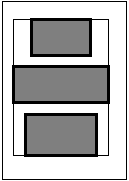
\includegraphics{bilder/bild_ganz}%
      \label{fig:bildpositionen2}%
    }%
    \hfil
    \caption{M�gliche Bildanordnungen}%
    \label{fig:bildpositionen}
  \end{figure}%
  \begin{figure}%
    \hfil
    \subfigure[mittig]{%
      
\includegraphics{bilder/bild_mitte}%
      \label{fig:nicht_bildpositionen_mitte}}%
    \hfil
    \subfigure[umflossen]{%
      
\includegraphics{bilder/bild_umflossen}%
      \label{fig:nicht_bildpositionen_umflossen}}%
    \hfil
    \subfigure[unten]{%
      
\includegraphics{bilder/bild_unten}%
      \label{fig:nicht_bildpositionen_unten}}%
    \hfil
    \caption{Verbotene Bildanordnungen}%
    \label{fig:nicht_bildpositionen}%
  \end{figure}%
\else
  \begin{figure}%
    \begin{minipage}{0.38\linewidth}
      \hfil
      \subfigure[oben]{%
        
\includegraphics{bilder/bild_oben}%
        \label{fig:bildpositionen1}%
      }%
      \hfil
      \subfigure[Bildseite]{%
        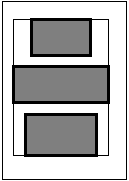
\includegraphics{bilder/bild_ganz}%
        \label{fig:bildpositionen2}%
      }%
     \hfil
      \caption{M�gliche Bildanordnungen}%
      \label{fig:bildpositionen}
    \end{minipage}%
    \hfill
    \begin{minipage}{0.57\linewidth}
      \hfil
      \subfigure[mittig]{%
        
\includegraphics{bilder/bild_mitte}%
        \label{fig:nicht_bildpositionen_mitte}}%
      \hfil
      \subfigure[umflossen]{%
        
\includegraphics{bilder/bild_umflossen}%
        \label{fig:nicht_bildpositionen_umflossen}}%
      \hfil
      \subfigure[unten]{%
        
\includegraphics{bilder/bild_unten}%
        \label{fig:nicht_bildpositionen_unten}}%
      \hfil
      \caption{Verbotene Bildanordnungen}%
      \label{fig:nicht_bildpositionen}%
    \end{minipage}%
  \end{figure}%
\fi
\makeatother

Bilder werden aus folgendem Grund niemals genau an der Stelle gesetzt,
an der auf sie verwiesen wird
(Bild~\ref{fig:nicht_bildpositionen_mitte}):
Wird ein Bild im Flie�text an einer Stelle definiert, an der nicht
gen�gend Platz verf�gbar ist, so muss das Bild auf die n�chste Seite
verschoben werden, wodurch eine gro�e L�cke in den Satz gerissen wird,
wie es Bild~\ref{fig:bild_zu_lang} zeigt.
%
\begin{figure}%
  \hfil
  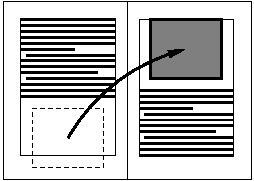
\includegraphics{bilder/bild_zu_lang}%
  \hfil
  {\Large \raisebox{38pt}{$\Longrightarrow$}}%
  \hfil
  
\includegraphics{bilder/bild_zu_lang2}%
  \hfil
  \caption[Entstehung gro�er L�cken im Text durch das Verschieben
  eines Bildes]{Beim Versuch, ein Bild an einer bestimmten Stelle in den
    Text zu setzen, tritt das Problem auf, dass es nicht mehr auf die
    Seite passt.
    Das Bild muss auf die n�chste Seite verschoben werden, was gro�e
    L�cken in den Text rei�t.}%
  \label{fig:bild_zu_lang}
\end{figure}%
%
Aus dem gleichen Grund d�rfen auch keine von Text umflossenen
Bilder\index{Bild!umflossen}
(Bild~\ref{fig:nicht_bildpositionen_umflossen}) erstellt werden.
Unten gesetzte Bilder (Bild~\ref{fig:nicht_bildpositionen_unten})
bereiten Probleme mit der Platzierung von Fu�noten und sollen unter
Anderem deshalb nicht verwendet werden.

Da das Bild nicht unbedingt dort erscheint, wo es im Text beschrieben
wird, soll auf jedes Bild verwiesen werden.
Das geschieht durch Formulierungen wie "`siehe Bild~\dots"', "`vgl.\
Bild~\dots"', "`wie in Bild~\dots\ skizziert"' oder einfach
durch die Bildnummer in Klammern "`(Bild~\dots)"'.
Damit der Verweis m�glich ist, erh�lt jedes Bild eine Bildunterschrift
mit laufender Nummer.
Die \emph{Bildunterschrift}\index{Bildunterschrift} wird, sofern sie
einzeilig ist, zentriert und ansonsten linksb�ndig mit h�ngendem
Einzug und Flattersatz gesetzt.
Als Beispiele f�r Bildunterschriften k�nnen einfach die in diesem
Dokument verwendeten Bilder dienen.

Da gerade beim Nachschlagen h�ufig zuerst ein Bild betrachtet wird,
bevor der Text gelesen wird, sollte die Bildunterschrift nicht zu
knapp ausfallen, sondern wenigstens eine kurze Beschreibung des
Gezeigten enthalten.
Enh�lt die Bildunterschrift einen oder mehrere ganze S�tze, so wird
sie mit einem Punkt abgeschlossen.
Enth�lt sie nur eine kurze Beschreibung ohne Pr�dikat, so wird kein
abschlie�ender Punkt gesetzt.

Bei der Erstellung der Bilder ist unbedingt darauf zu achten, dass
diese einheitlich gestaltet werden.
Das bezieht beispielsweise Liniendicken, Schrifarten und "=gr��en ein.
Eine Schriftgr��e von $\np[pt]{9}$ in den Zeichnungen entspricht der
der Bildunterschriften und ist daher eine geeignete Wahl.

H�ufig ist es notwendig, innerhalb eines Bildes
Teilbilder\index{Bild!Teilbild} zu
verwenden, die unter Umst�nden mit eigenen Bildunterschriften versehen
werden (beispielsweise in Bild~\ref{fig:bildpositionen}).
Die Unter"=Bildunterschriften werden alphanumerisch nummeriert und im
Schriftgrad 9~Punkt gesetzt.
Die Anordnung der Teilbilder kann je nach Gr��e und Bedarf neben"=
oder untereinander erfolgen.


% ===================================================================
\section{Tabellen}%
\label{sec:tabellen}%
\index{Tabelle}%

F�r Tabellen gelten viele der f�r Bilder gesagten Dinge ebenso.
Auch sie werden nur am oberen Rand bzw.\ auf einer
eigenen Seite platziert, sowie horizontal zentriert gesetzt.
Im Gegensatz zu Bildern haben Tabellen aber eine
�berschrift\index{Tabellen�berschrift}, die~-- wie der Name schon
sagt~-- �ber der eigentlichen Tabelle steht.

Wie im professionellen Buchsatz �blich, werden zur Unterteilung
ausschlie�lich horizontale Linien\index{Tabelle!Linie}
unterschiedlicher Dicke verwendet.
Spalten\index{Tabelle!Spalte} werden durch Zwischenr�ume voneinander
getrennt.
Tabelle~\ref{tab:tabelle_beispiel} zeigt ein Beispiel.
%
\begin{table}%
  \def\wn{\hphantom{\ensuremath{0}}}%
  \centering
  \caption{Als Beispiel einer Tabelle: Elastische Konstanten f�r
    verschiedene Einkristalle}%
  \label{tab:tabelle_beispiel}%
  \small
  \begin{tabular}{l*{7}{>{$}c<{$}}}
    \toprule
    \multicolumn{8}{c}{\bfseries Materialien mit kubischer
      Gitterstruktur}\\
    \midrule
    Material& E_{\mathrm{isotr.}}& E_{\langle
      100\rangle}& E_{\langle 111\rangle}& A& C_{11}& C_{12}& C_{44}\\
    Einheit&\mathrm{GPa}& \mathrm{GPa}& \mathrm{GPa}& &
    \mathrm{GPa}& \mathrm{GPa}& \mathrm{GPa}\\
    \midrule
    \multicolumn{8}{c}{Metalle und Halbmetalle}\\
    \midrule
    Al& \wn70& \wn\wn64& \wn\wn76&
    1,23& \wn108& \wn61& \wn29\\
    Au& \wn78& \wn\wn43& \wn117& 1,89& \wn186&
    157& \wn42\\
    Cu& 121& \wn\wn67& \wn192& 3,22& \wn168&
    121& \wn75\\
    $\alpha$"=Fe&  209& \wn129& \wn276& 2,13&
    \wn233& 124& 117\\
    Ni& 207& \wn137& 305& 2,50& \wn247& 147& 125\\
    Si& -& \wn130& 188& 1,57& \wn166& \wn64& \wn80\\
    W& 411& \wn411& \wn411& 1,00& \wn501& 198&
    151\\
    \midrule
    \multicolumn{8}{c}{Keramiken}\\
    \midrule
    Diamant&-& 1050& 1200& 1,20& 1076& 125& 576\\
    MgO& 310& \wn247& \wn343& 1,54&
    \wn291& \wn90& 155\\
    NaCl& \wn37& \wn\wn44&
    \wn\wn32& 0,72& \wn\wn49& \wn13& \wn13\\
    TiC& -& \wn476& \wn429& 0,88& \wn512&
    110& 117\\
    \midrule[\heavyrulewidth]
    \multicolumn{8}{c}{\bfseries Materialien mit
      hexagonaler Gitterstruktur}\\
    \midrule
    Material& E_{\mathrm{isotr.}}& \!\!\!\!\!C_{11}=C_{22}\!\!\!\!\!&
    C_{33}& C_{44}& \!\!\!\!\!C_{55}=C_{66}\!\!\!\!\!& C_{12}&
    \!\!\!\!\!C_{13}=C_{23}\!\!\!\!\!\\
    Einheit&\mathrm{GPa}& \mathrm{GPa}& \mathrm{GPa}&
    \mathrm{GPa}& \mathrm{GPa}& \mathrm{GPa}&
    \mathrm{GPa}\\
    \midrule
    Zn& \wn86& 143& \wn50& \wn40& \wn63& \wn17& \wn33\\
    \bottomrule
  \end{tabular}
\end{table}%

Verwenden Sie auch die horizontalen Linien sparsam.
Es ist zum Erstellen einer �bersichtlichen Tabelle nicht notwendig,
alle Zeilen durch Linien zu trennen.
F�gen Sie nur dann horizontale Linien ein, wenn ein inhaltlicher
Unterschied zwischen aufeinander folgenden Zeilen besteht.

Wenn m�glich, werden Einheiten nur einmal im Tabellenkopf angegeben
und anschlie�end nur die entsprechenden Zahlenwerte geschrieben.
Achten Sie auch in Tabellen darauf, ob eine Zahl als Formel oder als
Text angesehen werden soll, da sich, wie in
Abschnitt~\ref{sec:schrift} beschrieben, ihr Aussehen entsprechend
ver�ndern kann.

Unter Umst�nden k�nnen Tabellen sehr lang werden, so dass sie nicht
auf eine Seite passen. 
In diesem Fall k�nnen Tabellen �ber mehr als eine Seite gesetzt
werden.
In jedem Fall muss dann der Tabellenkopf auf jeder Seite wiederholt
werden.
Auf jeder Seite soll die Tabelle mit einer horizontalen Linie
abgeschlossen werden.
Zus�tzlich kann ein Hinweis darauf gegeben werden, dass die Tabelle
auf der n�chsten Seite fortgesetzt wird.

                                
% ===================================================================

%%% Local Variables: 
%%% mode: latex
%%% TeX-master: "richtlinien"
%%% End: 

%
% bgteubner class bundle
%
% textelemente.tex
% Copyright 2003--2012 Harald Harders
%
% This program may be distributed and/or modified under the
% conditions of the LaTeX Project Public License, either version 1.3
% of this license or (at your opinion) any later version.
% The latest version of this license is in
%    http://www.latex-project.org/lppl.txt
% and version 1.3 or later is part of all distributions of LaTeX
% version 1999/12/01 or later.
%
% This program consists of all files listed in manifest.txt.
% ===================================================================

\chapter{Weitere Textelemente}%
\label{sec:textelemente}%
\index{Textelement}%

In diesem Kapitel werden einige Textelemente, wie z.\,B. Beispiele,
Aufgaben oder Anmerkungen, besprochen.

% -------------------------------------------------------------------
\section{Aufz�hlungen}%
\label{sec:aufzaehlungen}%
\index{Aufz�hlung}

Aufz�hlungen k�nnen sowohl nummeriert als auch unnummeriert vorliegen.
Allgemein werden sie einger�ckt und k�nnen geschachtelt auftreten. 
Es sollte jedoch darauf geachtet werden, die Verschachtelungstiefe
nicht zu gro� werden zu lassen.

Je nachdem, wie lang die einzelnen Punkte der Aufz�hlungen sind,
k�nnen die vertikalen Abst�nde unterschiedlich gew�hlt werden.
F�r sehr lange Eintr�ge bietet es sich an, sowohl am Beginn der Liste
als auch zwischen den einzelnen Punkten einen vertikalen Zwischenraum
einzuf�gen, wie es das folgende Beispiel zeigt:
\begin{itemize}
\item Hier wird vor dem ersten Eintrag, zwischen den Eintr�gen und
  nach dem letzten Eintrag ein vertikaler Zwischenraum eingef�gt.
\item Bei kurzen Eintr�gen wirkt der Text durch die Zwischenr�ume
  l�chrig.
\end{itemize}

Sind die Eintr�ge k�rzer, so bietet es sich an, nur vor und nach der
Aufz�hlung einen Zwischenraum einzuf�gen, zwischen diesen aber nur
einen normalen Zeilenabstand:
\begin{itemize*}
\item Vor dem ersten Aufz�hlungspunkt ist ein Zwischenraum,
\item zwischen den Eintr�gen nicht, und
\item nach dem letzten Eintrag ist wieder Zwischenraum eingef�gt.
\end{itemize*}

Sind die Eintr�ge sehr kurz und vielleicht in einen Satz eingebettet,
der �ber die Aufz�hlung hinausgeht, so sollte weder
\begin{compactitem}
\item vor noch
\item zwischen noch
\item nach
\end{compactitem}
den einzelnen Punkten ein Zwischenraum eingef�gt werden.

Wie bei abgesetzten Formeln ist bei Aufz�hlungen darauf zu achten, ob
f�r den folgenden Text ein neuer Absatz begonnen werden soll oder
nicht.
Bei den beiden ersten Aufz�hlungen in diesem Abschnitt ist dies der
Fall, bei der dritten nicht.

Das folgende Beispiel zeigt die Kennzeichnung der Punkte in einer
nummerierten Aufz�hlung:
\begin{compactenum}
\item Die erste Ebene wird mit arabischen Zahlen nummeriert. 
  \begin{compactenum}
  \item In der zweiten Ebene werden Kleinbuchstaben verwendet.
    \begin{compactenum}
    \item Die dritte Ebene wird mit kleinen r�mischen Zahlen gekennzeichnet.
    \end{compactenum}
  \end{compactenum}
\end{compactenum}

F�r eine unnummerierte Aufz�hlung werden folgende Zeichen verwendet:
\begin{compactitem}
\item Die erste Ebene erh�lt einen gro�en Punkt.
  \begin{compactitem}
  \item F�r die zweite Ebene werden Spiegelstriche verwendet.
    \begin{compactitem}
    \item Die dritte Ebene wird mit Sternen gekennzeichnet.
    \end{compactitem}
  \end{compactitem}
\end{compactitem}
                                
% -------------------------------------------------------------------
\section{Beispiele}%
\label{sec:beispiele}%
\index{Beispiel}%

Es sind zwei M�glichkeiten zum Setzen von Beispielen vorgesehen:
Entweder werden Beispiele ohne typographische Kennzeichnung im
Flie�text gesetzt.
Dann muss jedoch darauf geachtet werden, dass der Anfang und das Ende
des Beispiels aus dem Text eindeutig ersichtlich sind.
Die zweite M�glichkeit, Beispiele zu kennzeichnen, besteht darin, sie
optisch vom Flie�text abzusetzen.
Dazu wird eine �berschrift gesetzt, die mit dem Wort "`Beispiel"'
beginnt. 
Es k�nnen optional eine Beispielnummer und ein Titel folgen,
wie im folgenden Beispiel illustriert:
\begin{example}[Ein Beispielbeispiel]
  \label{bsp:beispiel1}%
  Ein Beispiel wird links und rechts einger�ckt.
  Im Gegensatz zu alten Versionen der Dokumentklasse werden Beispiele
  per Default in normaler Schriftgr��e und mit normalem Zeilenabstand
  gesetzt.
  Dies kann jedoch umgeschaltet werden (vgl.\
  Abschnitt~\ref{sec:tex:aufbau}).
\end{example}
Das folgende Beispiel zeigt, wie Beispiele mit kleiner Schriftgr��e
aussehen.
\begingroup
  \makeatletter
  \def\theoremfont{\small}%
  \ifhhcls@times
    \def\theoremspacing{1.12}%
  \else
    \def\theoremspacing{1.06}%
  \fi
  \makeatother
  \begin{example}[Kleine Schrift]
    Mit der Schriftgr��e 9~Punkt sieht das Beispiel so aus.
    Wegen der kleinen Schrift wird der (relative) Zeilenabstand etwas
    erh�ht, um die Lesbarkeit zu gew�hrleisten.
  \end{example}
\endgroup
Beide Setzarten haben Vor- und Nachteile.
Zum einen suggeriert die kleinere Schrift (unter Umst�nden ungewollt),
dass der Inhalt der entsprechenden Umgebung unwichtig sei.
Andererseits kann es bei normalgro�er Schrift passieren, dass der
Leser bei langen Beispielen mit Seitenumbruch nicht merkt, dass er
noch innerhalb des Beispiels ist.

Auf nummerierte Beispiele kann dann eine Referenz gesetzt werden
(vgl.\ Beispiel~\ref{bsp:beispiel1}).

Ein nicht nummeriertes Beispiel sieht so aus:
\begin{example*}[Noch ein Beispielbeispiel]
  Auf ein nicht nummeriertes Beispiel kann nat�rlich, au�er �ber die
  Seitenzahl, nicht im Text verwiesen werden.
\end{example*}

Die Nummerierung eines Beispiels besteht aus der Kapitelnummer und der
Nummer des Beispiels innerhalb des aktuellen Kapitels.
Im n�chsten Kapitel wird die Z�hlung erneut bei 1 begonnen.

% -------------------------------------------------------------------
\section{S�tze, Lemmata, Definitionen usw.}%
\index{Anmerkung}%
\index{Satz}%
\index{Lemma}%

Au�er Beispielen gibt es noch einige weitere Dinge, die durch
abgesetzte Formatierung hervorgehoben werden k�nnen. 
Dazu z�hlen S�tze, Lemmata, Definitionen usw.
Sie werden wie Beispiele gesetzt, nur nat�rlich mit den entsprechenden
�berschriften.
Eine eventuelle Nummerierung erfolgt getrennt nach den einzelnen
Typen.

H�ufig m�chte man dem Leser weiterf�hrende Informationen geben, die
nicht unbedingt zum Verst�ndnis des Buches notwendig sind.
Hier kann es zweckm��ig sein, diese in einer kleineren Schrift
($\np[pt]{8}$) zu setzen und links und rechts einzur�cken, um sie vom
�brigen Text abzuheben.
\begin{advanced}
  Durch diese Auszeichnung 
  wird dem Leser suggeriert, dass dieser Text unter Umst�nden nicht
  ganz so wichtig ist.
  Deshalb sollte diese Variante auch nur dann verwendet werden, wenn
  der in der Anmerkung enthaltene Text nicht unbedingt f�r das
  Verst�ndnis des Buches notwendig ist.

  Wenn man diese Formatierungsart verwendet, ist es zwingend
  notwendig, dass der Leser im Vorwort oder in der Einleitung darauf
  hingewiesen wird, dass die so gesetzten Bereiche Erg�nzungen bzw.\
  Anmerkungen sind, die f�r das Verst�ndnis des Buches nicht unbedingt
  notwendig sind.
\end{advanced}

Wenn man diese Art der Auszeichnung verwendet, muss dringend darauf
geachtet werden, dass sich der Text sowohl dann sinnvoll und fl�ssig
liest, wenn man die Anmerkung mitliest, als auch dann, wenn man sie
ausl�sst.

Manche Autoren m�chten besonders wichtige Gleichungen und Textpassagen
durch einen grauen Hintergrund hervorheben.
Auch dies ist m�glich.
\begin{example}
  \label{bsp:important}%
  Wenn man sich st�ndig Textbeispiele ausdenken muss, gehen einem
  irgendwann die Ideen aus.
  %
  \begin{important}
    Das ist nicht besonders angenehm.
    \begin{align*}
      \sin^2\alpha + \cos^2\alpha &= 1\,.\quad\text{(eine beliebige Formel)}
    \end{align*}%
  \end{important}
  %
  Da dieser Satz inhaltlich dazu geh�rt, ist er ohne Absatzeinzug
  gesetzt.
  %
  \begin{important*}
    \begin{align*}
      \sin^2\alpha + \cos^2\alpha &= 1\,.\quad\text{(eine beliebige Formel)}
    \end{align*}
    Es muss inhaltlich entschieden werden, ob ein Absatz folgt oder
    nicht.\footnote{Warum hier zwei graue K�sten gezeigt werden, eine
      mit Text am Anfang, die andere mit einer abgesetzten Gleichung
      am Anfang, wird in Abschnitt~\ref{sec:tex:important} deutlich.}
  \end{important*}

  Da dieser Satz nichts mit dem Rest zu tun hat, beginnt mit ihm ein
  neuer Absatz.
  Das ist am Absatzeinzug zu erkennen.
\end{example}

Diese grau hinterlegten Boxen sollten kurz gehalten werden, da in
ihnen normalerweise kein Seitenumbruch auftreten soll.

% -------------------------------------------------------------------
\section{Aufgaben und L�sungen}%
\label{sec:aufgaben}%
\index{Aufgabe}%
\index{L�sung}%

F�r Lehrb�cher ist es sinnvoll, im Buch Aufgaben zu stellen, f�r die
direkt danach oder an anderer Stelle L�sungen vorhanden sind.
Es ist dabei m�glich, eine globale Aufgabensammlung am Ende des Buches zu
erstellen oder Aufgabensammlungen am Ende jeden Kapitels zu erstellen.
Sie sollten sich f�r eine der beiden Varianten entscheiden.

% -------------------------------------------------------------------
\subsection{Globale Aufgabensammlung}%
\label{sec:aufgabensammlung_global}%
\index{Aufgabensammlung!global}%

Eine globale Aufgabensammlung kann zweckm��igerweise zwischen dem
Textteil und dem Anhang des Buches gesetzt werden.
Dabei ist es denkbar, einen Teil mit dem Titel "`�bungsteil"'
einzurichten, in dem dann zwei Kapitel enthalten sind, n�mlich
"`Aufgaben"' und "`L�sungen"'.
Eine andere M�glichkeit besteht darin, einfach als letztes Kapitel das
Kapitel "`Aufgaben"' zu setzen und dann am Ende des Anhangs das
Kapitel "`L�sungen"'.
Schlie�lich ist es auch denkbar, nur ein Kapitel "`Aufgaben"' zu
definieren, in dem die L�sungen jeweils direkt auf die entsprechenden
Aufgaben folgen.
Auf jeden Fall sollte am Beginn des Kapitels "`Aufgaben"' darauf
verwiesen werden, an welcher Stelle die L�sungen gefunden werden
k�nnen.

F�r eine globale Aufgabensammlung ist es sinnvoll, die Aufgaben
zu nummerieren, wie es in folgendem Beispiel getan wird:
\begin{exercise}{Buch erstellen}
  \label{auf:beispiel1}%
  Erstellen Sie ein Buch zur Ver�ffentlichung im Teubner Verlag!
  Dabei sind die Autorenrichtlinien, die sie gerade lesen, zu
  beachten.
\end{exercise}
\bigskip

Da diese Art der Formatierung daf�r gedacht ist, dass nur Aufgaben und
L�sungen aufeinander folgen und kein normaler Text eingemischt ist
(was an dieser Stelle demnach falsch gemacht wird\footnote{Daher wurde
  hier nach der Aufgabe ein Abschnittsabstand manuell eingef�gt.}),
ist keine Textauszeichnung durch Einr�ckungen o.\,�.\ notwendig.
Die �berschrift der Aufgabe entspricht Abschnitts�berschriften, ein
Titel ist obligatorisch.\footnote{Wer partout keinen Titel haben
  m�chte, kann ihn auch leer definieren.
  Allerdings ist es dann nicht sinnvoll, die Aufgaben ins
  Inhaltsverzeichnis aufzunehmen oder ein Verzeichnis der Aufgaben zu
  erstellen.}

Wenn die entsprechende L�sung direkt auf die Aufgabe folgt, kann eine
Nummerierung der Aufgaben auch entfallen, wie im folgenden Beispiel:
\begin{exercise*}{Stichwortverzeichnis}
  Erstellen Sie f�r Ihr Buch ein Stichwortverzeichnis!
  Achten Sie darauf, dass es sinnvoll und nicht zu kurz wird!
\end{exercise*}
\bigskip

L�sungen werden mit einem kleineren Schriftgrad gesetzt, um Platz zu
sparen.
Unnummerierte L�sungen k�nnen (wie hier gezeigt), m�ssen jedoch nicht,
einen Titel erhalten:
\begin{answer*}[Stichwortverzeichnis]
  Die L�sung der Aufgabe kann ich Ihnen leider nicht abnehmen.
  Lesen Sie aber auf jeden Fall Abschnitt~\ref{sec:tex_index}
  aufmerksam durch.
\end{answer*}
\bigskip

Eine unnummerierte L�sung muss direkt auf die entsprechende Aufgabe
folgen, da sonst eine Zuordnung nicht m�glich ist.

F�r nummierierte L�sungen gilt das selbe (hier ohne Titel):
\begin{answer}{auf:beispiel1}
  Die L�sung zu dieser Aufgabe ist, wie Sie sicherlich schon gemerkt
  haben, mit gro�em Aufwand verbunden.
  Bei der Erstellung dieser Autorenrichtlinien merke auch ich dies
  aufs Neue.
\end{answer}
\bigskip

Bei allen in diesem Abschnitt gezeigten Beispielen besteht das
Problem, dass der �bergang von Aufgabe bzw.\ L�sung zu normalem Text
schwierig zu finden ist.
Aus diesem Grund sind so formatierte Aufgaben auch nur in Aufgaben"=
und L�sungssammlungen zu verwenden, in denen auf eine Aufgabe nur eine
weitere Aufgabe oder eine L�sung folgen kann.

% -------------------------------------------------------------------
\subsection{Aufgaben am Ende jeden Kapitels}%
\index{Aufgabensammlung!kapitelweise}%

Soll am Ende jeden Kapitels eine Aufgabensammlung erstellt werden, so
besteht die Aufgabennummer aus der Kapitelnummer und der
Aufgabennummer.
Die Aufgabensammlung kann in einem eigenen Abschnitt,
beispielsweise "`Aufgaben"', zusammengefasst werden.

Einige Beispiele:
\begin{subexercise}{Buch erstellen}
  \label{auf:beispiel2}%
  Erstellen Sie ein Buch zur Ver�ffentlichung im Teubner Verlag!
  Dabei sind die Autorenrichtlinien, die sie gerade lesen, zu
  beachten.
\end{subexercise}
\begin{subanswer}{auf:beispiel2}
  Die L�sung zu dieser Aufgabe ist, wie Sie sicherlich schon gemerkt
  haben, mit gro�em Aufwand verbunden.
  Bei der Erstellung dieser Autorenrichtlinien merke auch ich dies
  aufs Neue.
\end{subanswer}
\begin{subexercise*}{Stichwortverzeichnis}
  Erstellen Sie f�r Ihr Buch ein Stichwortverzeichnis!
  Achten Sie darauf, dass es sinnvoll und nicht zu kurz wird!
\end{subexercise*}
\begin{subanswer*}[Stichwortverzeichnis]
  Die L�sung der Aufgabe kann ich Ihnen leider nicht abnehmen.
  Lesen Sie aber auf jeden Fall Abschnitt~\ref{sec:tex_index}
  aufmerksam durch.
\end{subanswer*}


% -------------------------------------------------------------------
\subsection{Teilaufgaben}%
\index{Aufgabe!Teil-}%

H�ufig ist es zweckm��ig, innerhalb einer Aufgabe Teilaufgaben zu
definieren.
Diese werden mit Buchstaben, gefolgt von einer Klammer, bezeichnet,
wie im folgenden Beispiel:
\begin{subexercise*}{Mal wieder Buch erstellen}
  \label{auf:teilaufgaben}%
  Zur Erstellung eines Buches sollen folgende Dinge erledigt werden:
  \begin{subtask}
  \item Recherchieren Sie gr�ndlich!
  \item Schreiben Sie den Text, ohne auf Formatierungen zu achten!
  \end{subtask}
  Wenn der inhaltliche Teil fertig ist, geht es an die optischen
  Dinge:
  \begin{subtask}
  \item Formatieren Sie den Text!
  \item Erstellen Sie die Verzeichnisse (Formelverzeichnis,
    Abk�rzungsverzeichnis, Literaturverzeichnis,
    Stichwortverzeichnis)!
  \end{subtask}
\end{subexercise*}

Wie im Beispiel zu sehen, werden die Teilaufgaben innerhalb einer
Aufgabe fortlaufend nummeriert, auch wenn Text zur Erl�uterung
eingef�gt ist.
Bei jeder Aufgabe beginnt die Nummerierung bei a).


% ===================================================================

%%% Local Variables: 
%%% mode: latex
%%% TeX-master: "richtlinien"
%%% End: 

%
% bgteubner class bundle
%
% verzeichnisse.tex
% Copyright 2003--2012 Harald Harders
%
% This program may be distributed and/or modified under the
% conditions of the LaTeX Project Public License, either version 1.3
% of this license or (at your opinion) any later version.
% The latest version of this license is in
%    http://www.latex-project.org/lppl.txt
% and version 1.3 or later is part of all distributions of LaTeX
% version 1999/12/01 or later.
%
% This program consists of all files listed in manifest.txt.
% ===================================================================
\chapter{Verzeichnisse}%
\index{Verzeichnis}%

Verzeichnisse nehmen im Buch eine gesonderte Stellung ein.
Sie enthalten keine eigentlichen Inhalte.
Stattdessen dienen sie zur Orientierung im Buch.
Da es verschiedene Herangehensweisen beim Konsultieren eines Buches
gibt, sind auch unterschiedliche Verzeichnisse notwendig.

Die Reihenfolge der einzelnen Verzeichnisse ist nicht exakt
festgelegt (bis auf das Stichwortverzeichnis, das als letztes
Verzeichnis gesetzt werden muss).
Eine m�gliche Reihenfolge\index{Verzeichnis!Reihenfolge} ist die
folgende:
Literaturverzeichnis, Formelzeichenverzeichnis, Abk�rzungsverzeichnis,
Abbildungsverzeichnis, Tabellenverzeichnis, Verzeichnis der
Beispiele, Aufgabenverzeichnis, Stichwortverzeichnis.

In den meisten F�llen sind aber einige dieser Verzeichnisse nicht
n�tig. 
So werden die meisten Leser nach einem Sachverhalt nicht im
Abbildungs"~, Tabellen"~, Aufgaben"~ oder Beispielverzeichnis suchen,
sondern das Stichwortverzeichnis konsultieren, in dem der im Bild
o.\,�.\ verwendete Begriff aufgef�hrt sein sollte.
Ein Formelzeichenverzeichnis beispielsweise sollte aber vorhanden
sein.

% -------------------------------------------------------------------
\section{Inhaltsverzeichnis}%
\index{Inhaltsverzeichnis|textbf}%

Das Aussehen des Inhaltsverzeichnisses kann am einfachsten anhand des
Inhaltsverzeichnisses dieser Anleitung studiert werden.

Einige Hinweise seien jedoch hier gegeben:
Teil"= und Kapitel�berschriften werden in unterschiedlichen
Schriftgraden fett gesetzt, dazu rechtsb�ndig fett die entsprechende
Seitenzahl.
Abschnitte sowie Unterabschnitte werden normal gesetzt.
Bei ihnen wird zus�tzlich eine Punktreihe bis zur Seitenzahl gesetzt.

Im Inhaltsverzeichnis sind auch die weiteren
Verzeichnisse wie Formel"~, Abk�rzungs"~, 
\feinschliff{Literatur"=,}{Literatur"~,}{Literatur"~,}{Literatur"~,}
Abbildungs"~,
Tabellen"~, sowie Stichwortverzeichnis eingetragen, sofern vorhanden.

Da das Inhaltsverzeichnis automatisch erzeugt wird, wird auf weitere
Einzelheiten verzichtet.

% -------------------------------------------------------------------
\section{Literaturverzeichnis}%
\index{Literaturverzeichnis|textbf}%

Im Literaturverzeichnis werden alle Literaturstellen, auf die im Buch
verwiesen wird, aufgef�hrt.
Es wird eine numerische Bezeichnung der Literaturstellen, jeweils in
eckigen Klammern, verwendet.
Titel werden kursiv gesetzt, alles andere normal aufrecht. 
Kapit�lchen werden normalerweise nicht verwendet.
Es wird Flattersatz eingesetzt, da ansonsten ein sehr unruhiges
Satzbild entstehen w�rde.
Da das Literaturverzeichnis automatisch erstellt wird, wird an dieser
Stelle auf eine genauere Beschreibung verzichtet.


% -------------------------------------------------------------------
\section{Abbildungsverzeichnis und Tabellenverzeichnis}%
\index{Abbildungsverzeichnis|textbf}%
\index{Tabellenverzeichnis|textbf}%

Das Abbildungsverzeichnis und das Tabellenverzeichnis werden als
unnummerierte Kapitel gesetzt, die im Anschluss an den Anhang
eingef�gt werden k�nnen.

Im Abbildungsverzeichnis werden alle im Buch vorhandenen Bilder
aufgelistet.
F�r jedes Bild wird die Bildnummer, die Bildunterschrift und die
Seitenzahl eingetragen.
Da die Bildunterschriften mitunter recht lang werden k�nnen, sollte
dann im Verzeichnis nur eine Kurzform der Bildunterschrift verwendet
werden.
F�r das Tabellenverzeichnis gilt dasselbe wie f�r das
Abbildungsverzeichnis.

Ob ein Abbildungsverzeichnis und ein Tabellenverzeichnis �berhaupt
erstellt werden soll, bleibt dem Autoren freigestellt.
Es m�ssen aber entweder beide oder keines der beiden Verzeichnisse
gedruckt werden.
Das Abbildungsverzeichnis muss direkt vor dem Tabellenverzeichnis
stehen und am Ende des Anhangs gesetzt werden.

Um Platz zu sparen, werden diese Verzeichnisse in einer
9~Punkt~Schrift gesetzt.

% -------------------------------------------------------------------
\section{Verzeichnisse der Beispiele und der Aufgaben usw.}%
\index{Verzeichnis der Beispiele|textbf}%
\index{Aufgabenverzeichnis|textbf}%

Diese Verzeichnisse werden wie das Abbildungsverzeichnis gesetzt.
Sie enthalten die in den Abschnitten~\ref{sec:beispiele} und
\ref{sec:aufgaben} eingef�hrten Beispiele, Aufgaben oder andere
entsprechend gesetzte Umgebungen.
Auch diese Verzeichnisse sind optional.

Wird eine zentrale Aufgabensammlung f�r das Buch verwendet, k�nnen die
Aufgaben auch ins Inhaltsverzeichnis statt in ein gesondertes
Aufgabenverzeichnis aufgenommen werden.

% -------------------------------------------------------------------
\section{Verwendete Formelzeichen}%
\label{sec:formelzeichen}%
\index{Formelzeichenverzeichnis|textbf}%

Im Formelzeichenverzeichnis werden tabellarisch alle wichtigen Formelzeichen
und Indizierungen des Buches aufgef�hrt und kurz erkl�rt oder benannt.
Dabei bleibt es dem Autoren freigestellt, ob er alle Formelzeichen
in eine gemeinsame Liste setzt, oder ob er einzelne, nach Themen
getrennte Listen (z.\,B.\ Skalare, Vektoren, Matrizen, \dots)
erstellt.

Ein Formelverzeichnis kann etwa so aussehen:
\begin{theglossary}[\subsection*{Skalare}]%
  %
  \item[$\alpha_{\mathrm{k}}$] Kerbformzahl
  %
  \item[$\varepsilon$] technische Dehnung
  %
  \item[$\varphi$] wahre Dehnung
  %
  \item[$\sigma$] Spannung
  %
  \item[$a$] Gitterkonstante
  \item[$a$] Rissl�nge bei Oberfl�chenrissen und halbe Rissl�nge bei inneren
  Rissen
  %
  \item[$c$] Gitterkonstante
  %
  \item[$K$] Spannungsintensit�tsfaktor
  %
  \item[$R_{\mathrm{eH}}$] obere Streckgrenze f�r Materialien mit ausgepr�gter
  Streckgrenze
  \item[$R_{\mathrm{eL}}$] untere Streckgrenze f�r Materialien mit
  ausgepr�gter Streckgrenze
  \item[$R_{\mathrm{m}}$] Zugfestigkeit
  \item[$R_{\mathrm{p0,2}}$] Dehngrenze f�r Materialien ohne ausgepr�gte
  Streckgrenze
  %
\end{theglossary}%

Es ist auch m�glich, Buchstaben zur Gliederung einzuf�gen:
\begin{theglossary}[\subsection*{Skalare}]%
  \glossarynewchar{Symbole}
  \item[$\alpha_{\mathrm{k}}$] Kerbformzahl
  \item[$\varepsilon$] technische Dehnung
  \item[$\varphi$] wahre Dehnung
  \item[$\sigma$] Spannung
  \glossarynewchar{A}
  \item[$a$] Gitterkonstante
  \item[$a$] Rissl�nge bei Oberfl�chenrissen und halbe Rissl�nge bei
    inneren Rissen
  \glossarynewchar{C}
  \item[$c$] Gitterkonstante
  \glossarynewchar{K}
  \item[$K$] Spannungsintensit�tsfaktor
  \glossarynewchar{R}
  \item[$R_{\mathrm{eH}}$] obere Streckgrenze f�r Materialien mit
    ausgepr�gter Streckgrenze
  \item[$R_{\mathrm{eL}}$] untere Streckgrenze f�r Materialien mit
  ausgepr�gter Streckgrenze
  \item[$R_{\mathrm{m}}$] Zugfestigkeit
  \item[$R_{\mathrm{p0,2}}$] Dehngrenze f�r Materialien ohne
    ausgepr�gte Streckgrenze
\end{theglossary}%

Im Formelverzeichnis sollen die Eintr�ge alphabetisch sortiert
sein.
Die Symbole, die sich nicht in das lateinische Alphabet einsortieren
lassen (z.\,B. griechische Zeichen), stehen davor und sind~-- soweit
m�glich~-- untereinander sortiert.

Das griechische Alphabet wird folgenderma�en sortiert:
$A\alpha$, $B\beta$, $\Gamma\gamma$, $\Delta\delta$,
\makeatletter
$E\varepsilon\iftimes{\ifhhcls@mathtime\epsilon\fi}{\epsilon}$,
\makeatother
$Z\zeta$, $H\eta$,
$\Theta\vartheta\theta$, $I\iota$, $K\kappa$, $\Lambda\lambda$,
$M\mu$, $N\nu$, $\Xi\xi$, $Oo$, $\Pi\pi$,
\makeatletter
$P\varrho\iftimes{\ifhhcls@mathtime\rho\fi}{\rho}$,
\makeatother
$\Sigma\sigma$, $T\tau$, $Y\upsilon$, $\Phi\varphi\phi$, $X\chi$,
$\Psi\psi$, $\Omega\omega$.

Ob nur ein Verzeichnis als unnummeriertes Kapitel erstellt wird, das
alle Formelzeichen enth�lt, oder ob ein unnummeriertes Kapitel
verwendet wird, in dem unterschiedliches Verzeichnisse als
unnummerierte Abschnitte eingef�gt werden, die beispielsweise nach
\emph{Skalaren}, \emph{Vektoren}, \emph{Tensoren} und \emph{Indizes
  und Operatoren} aufgeteilt sind, bleibt dem Autoren �berlassen.
Die Formelzeichenverzeichnisse werden in einer 8"=Punkt"=Schrift
gesetzt, um Platz zu sparen.
Da hier keine l�ngeren Passagen gelesen werden, ist eine so kleine
Schriftart ausreichend gro�.

% -------------------------------------------------------------------
\section{Abk�rzungsverzeichnis bzw.\ Glossar}%
\label{sec:abkuerzungsverzeichnis}%
\index{Abk�rzungsverzeichnis|textbf}%
\index{Glossar|see{Abk�rzungsverzeichnis}}%

Abk�rzungsverzeichnisse und Glossare werden wie
Formelzeichenverzeichnisse gesetzt. 
Ein Beispiel:
\begin{theglossary}[\subsection*{Abk�rzungsverzeichnis}]
  %
  \item[\acro{GEH}] Gestalt�nderungsenergiehypothese
  %
  \item[hdp] hexagonal dichtest gepackt
  %
  \item[kfz] kubisch fl�chenzentriert
  \item[krz] kubisch raumzentriert
  %
  \item[\acro{SH}] Schubspannungshypothese
  %
\end{theglossary}%


% -------------------------------------------------------------------
\section{Stichwortverzeichnis}%
\index{Stichwortverzeichnis|textbf}%

Das Stichwortverzeichnis wird zweispaltig in einer
8"~Punkt"=Schrift gesetzt.
Die Seitenzahlen, auf denen der jeweilige Begriff auftaucht, werden
durch ein Komma getrennt direkt an den Begriff angeh�ngt.
Das genaue Aussehen des Stichwortverzeichnisses kann am besten anhand
des Verzeichnisses am Ende dieser Anleitung studiert werden.

Einige wichtige Dinge beim Aufbau des Verzeichnisses sollen dennoch
hier beschrieben werden:
Es sollen nicht alle Stellen, an denen ein Begriff im Buch vorkommt,
in das Stichwortverzeichnis aufgenommen werden, sondern nur
diejenigen, an denen der Begriff eingef�hrt oder ma�geblich verwendet
wird.
Auch wenn der Begriff selbst nur in einer Kapitel"= oder
Abschnitts�berschrift vorkommt, soll er im Stichwortverzeichnis
vorkommen, sofern er dort wichtig ist.\footnote{Mir ist einmal ein Buch
  untergekommen, in dem der Begriff \emph{Schwei�en} im
  Stichwortverzeichnis zwar vorkam, aber nur auf eine Seite verwies,
  auf der der Begriff zwar stand, aber fast nichts �ber Schwei�en
  geschrieben wurde. 
  Die Seitenzahl des Kapitels �ber Schwei�en war daf�r aber nicht im
  Stichwortverzeichnis enthalten.
  So etwas darf nicht vorkommen.}
Die Seitenzahl f�r einen besonders wichtigen Eintrag kann fett
gedruckt werden, z.\,B.
\begin{quotation}
  \bsptheindex
  \begin{theindex}
  \item Stichwortverzeichnis, \textbf{27}, 34, 35
  \end{theindex}
\end{quotation}

Existieren f�r einen Begriff auch andere Beschreibungen, so sollen
alle m�glichen W�rter, unter denen man diesen Begriff suchen k�nnte,
im Stichwortverzeichnis aufgef�hrt werden.
Es kann dann ein Verweis auf denjenigen Begriff gesetzt werden, der im
Dokument verwendet wird, z.\,B.
\begin{quotation}
  \bsptheindex
  \begin{theindex}
  \item Cosinus, \see{Trigonometrische Funktion}{15}

  \indexspace
  \item Sinus, \see{Trigonometrische Funktion}{15}

  \indexspace
  \item Tangens, \see{Trigonometrische Funktion}{15}
  \item Trigonometrische Funktion, 15

  \indexspace
  \item Winkelfunktion, 23, \seealso{Trigonometrische Funktion}{15}
  \end{theindex}
\end{quotation}
Seien Sie hier nicht zu sparsam. Es ist nichts �rgerlicher, als einen
Begriff im Stichwortverzeichnis nicht zu finden, nur weil man einen
etwas anderen Begriff als der Autor des Buches verwendet!
Meine eigene Erfahrung ist es, dass man in den meisten F�llen �ber das
Stichwortverzeichnis nach Inhalten in einem Buch sucht.
Daher ist es besonders wichtig, dass ein Buch ein gutes
Stichwortverzeichnis enth�lt.

H�ufig kommt es vor, dass zu einem �berbegriff einige Unterbegriffe
existieren.
Diese Tatsache sollte auch beim Setzen des Stichwortverzeichnisses
ber�cksichtigt werden, beispielsweise so:
\begin{quotation}
  \bsptheindex
  \begin{theindex}
  \item Cosinus, 15
    \subitem Hyperbolicus, 15

    \indexspace
  \item Sinus, 15

    \indexspace
  \item Tangens, 16, \seealso{Trignonometrische Funktion\subind
      Tangens}{16}\label{ind:bsp1}
  \item Trigonometrische Funktion, 15, 16
    \subitem Cosinus, 15
    \subsubitem Hyperbolicus, 15
    \subitem Sinus, 15
    \subitem Tangens, 16
  \end{theindex}
\end{quotation}
Wie im Beispiel zu erkennen, gibt es zwei Stufen f�r Unterbegriffe.
Dennoch sollten die Unterbegriffe h�ufig zus�tzlich in der Hauptebene
aufgenommen werden.

Soll ein Verweis auf einen Unterbegriff vorgenommen werden, so wird
dieser wie im Beispiel bei "`\seealso{Trignonometrische
  Funktion\subind Tangens}{16}"' mit einem Gedankenstrich vom
Hauptbegriff getrennt.

% ===================================================================
% Dateiende


%%% Local Variables: 
%%% mode: latex
%%% TeX-master: "bgteubner"
%%% End: 


\addpart{Durchf�hrung mit \LaTeX\label{part:latex}}
%
% bgteubner class bundle
%
% tex_globales.tex
% Copyright 2003--2012 Harald Harders
%
% This program may be distributed and/or modified under the
% conditions of the LaTeX Project Public License, either version 1.3
% of this license or (at your opinion) any later version.
% The latest version of this license is in
%    http://www.latex-project.org/lppl.txt
% and version 1.3 or later is part of all distributions of LaTeX
% version 1999/12/01 or later.
%
% This program consists of all files listed in manifest.txt.
% ===================================================================
\chapter{Globales}%
\texindex{Globales}%

Zur Erstellung der B�cher f�r den Teubner Verlag werden die
Dokumentklasse \verb|bgteubner| sowie einige weitere Dateien, wie
zus�tzliche notwendige Pakete, zur Verf�gung gestellt.
Wie sie installiert werden k�nnen, ist in einer Installationsanleitung
ab Seite~\pageref{chap:installation} erl�utert.
In diesem Teil der Anleitung wird dargestellt, wie das im vorigen Teil
vorgestellte Layout mit \LaTeX\ verwirklicht wird.

% ===================================================================
\section{Aufbau des Dokumentes}%
\label{sec:tex:aufbau}%
\texindex{Aufbau}%

Zur Erstellung eines Buches wird die Dokumentklasse
\verb|bgteubner.cls|\clsindex{bgteubner.cls} verwendet, die am Beginn
des Dokuments mit folgender Zeile aufgerufen wird:
\begin{verbatim}[\small\makeescape\|\makebgroup\[\makeegroup\]]
\documentclass|oarg[Sprachen,Optionen]{bgteubner}
\end{verbatim}
\macroindex{documentclass}%
Als Sprachen m�ssen alle im Dokument verwendeten Sprachen angegeben
werden.
Dazu geh�ren auch alle im Literaturverzeichnis vorkommenden Sprachen.
Die "`Hauptsprache"' des Buchs wird als \emph{letzter} Eintrag
angegeben.
Beispielsweise f�hrt der Eintrag
\begin{verbatim}[\small]
\documentclass[frenchb,english,ngerman]{bgteubner}
\end{verbatim}
\optindex{frenchb}\optindex{english}\optindex{ngerman}%
zu einem deutschen Buch nach neuen Rechtschreibregeln, in dem
englische und franz�sische Sprachabschnitte erlaubt sind.
Sollte das Buch noch nach alten Regeln geschrieben werden, so kann
statt \verb|ngerman| \verb|german|\optindex{german} verwendet werden.
Es ist nicht notwendig und nicht zul�ssig, eine Sprache explizit mit
einem der Pakete \verb|babel|\styindex{babel} oder \verb|(n)german| zu
w�hlen, da die Klasse \verb|bgteubner| schon alles notwendige
einstellt.\footnote{Intern wird \texttt{babel} verwendet.}
Sollten franz�sische Abschnitte oder Literaturverweise vorkommen, so
verwenden Sie bitte die Sprachoption \verb|frenchb| statt
\verb|french|, da das \verb|babel|"=Paket dort einen Bug enth�lt, der
bei \verb|frenchb| nicht auftritt.

Als \meta{Optionen} k�nnen unterschiedliche Dinge dienen.
Tabelle~\ref{tab:klassenoptionen} gibt einen �berblick.
%
\begin{table}%
  \begin{minipage}{\linewidth}
  \centering
  \def\default{{\rmfamily*}}%
  \caption{Klassenoptionen der Klasse \texttt{bgteubner}.
    Defaultm��ig aktivierte Optionen sind mit einem \default\
    gekennzeichnet.}%
  \index{MathTime}%
  \index{MathTimePlus|see{MathTime}}%
  \index{Y\,\&\,Y!MathTime|see{MathTime}}%
  \label{tab:klassenoptionen}%
  \begin{tabular}{>{\ttfamily}ll}
    \toprule
    \rmfamily Option& Erkl�rung \\
    \midrule
    a5paper& Papiergr��e \acro{DIN"~A\,5}, vgl.\
    Abschnitt~\ref{sec:seitenformat} \\
    17x24paper\default& Papiergr��e $\np[mm]{170}\times\np[mm]{240}$,
    vgl.\ Abschnitt~\ref{sec:seitenformat} \\
    \midrule
    times\default & Verwendung der Times als Brotschrift, vgl.\
    Abschnitt~\ref{sec:schrift} \\
    mathtime & Verwendung der Times als Brotschrift mit MathTime- und
    MathTimePlus"=\\
    & Schriften von Y\,\&\,Y\footnote{Die MathTime"= und
      MathTimePlus"=Schriftfamilien verbessern den mathematischen
      Schriftsatz erheblich. Sie sind bei Y\,\&\,Y
      (\url{http://www.yandy.com}) kommerziell erh�ltlich. Es wird nur die
      vollst�ndige Kombination aus MathTime und MathTimePlus
      unterst�tzt.}, vgl.\ Abschnitt~\ref{sec:schrift} \\
    cm& European Computer Modern als Brotschrift, vgl.\
    Abschnitt~\ref{sec:schrift} \\
    \midrule
    arrowvec\default & Vektoren mit Pfeil, Matrizen doppelter Pfeil,
    vgl.\ Abschn.~\ref{sec:mathematik} \\
    boldvec& Vektoren und Matrizen fett,
    vgl.\ Abschn.~\ref{sec:mathematik} \\
    ulinevec& Vektoren einmal, Matrizen doppelt unterstrichen,
    vgl.\ Abschn.~\ref{sec:mathematik} \\
    \midrule
    greybox& Graue K�sten wie Beispiel~\ref{bsp:important} zulassen \\
    exercisetotoc& Aufgaben ins Inhaltsverzeichnis \\
    answertotoc& L�sungen (und Aufgaben) ins Inhaltsverzeichnis \\
    draft& Entwurfsstadium \\
    titlepage& Setzt die Titelseite auch ohne die Option
    \texttt{draft} \\
    \midrule
    normaltheorem\default & Setzt theoremartige Umgebungen in normaler
    Schriftgr��e \\
    smalltheorem & Setzt theoremartige Umgebungen in \cs{small} \\
    \bottomrule
  \end{tabular}
\end{minipage}
\end{table}%
%
Die meisten Optionen sollten ohne weitere Erkl�rung verst�ndlich sein.

Die Option \texttt{draft} ver�ndert einige Kleinigkeiten.
Ist sie gesetzt, kann ein Titelblatt erzeugt werden, auf dem die
Autoren, der Titel, die Auf"|lage sowie das �bersetzungsdatum gesetzt
werden.
Weiterhin wird auf fast allen Seiten am unteren Papierrand gesetzt,
wann das Dokument �bersetzt wurde.
Schlie�lich werden Zeilen mit einem schwarzen Balken markiert, in
denen der Umbruchalgorithmus von \LaTeX\ kein zufriedenstellendes
Ergebnis erzielen konnte.\footnote{Dazu mehr in
  Abschnitt~\ref{sec:tex_silbentrennung}.}
Die Option \texttt{draft} wird \emph{nicht} an das
\texttt{graphics}"=Paket weitergereicht, so dass trotz gesetzer
\texttt{draft}"=Option die mit \cs{includegraphics} eingebundenen
Bilder wirklich eingebunden werden.
M�chten Sie, um Zeit zu sparen, nur Platzhalter angezeigt bekommen,
k�nnen Sie dies erreichen, indem Sie \emph{vor der}
\cs{documentclass}"=Zeile folgende Zeile einf�gen:
\begin{verbatim}[\small]
\PassOptionsToPackage{draft}{graphicx}
\end{verbatim}
Mit der Option \texttt{titlepage} wird das Titelblatt ohne die
anderen Auswirkungen von \texttt{draft} gesetzt.

Zur �bergabe an den Verlag darf weder die Option \texttt{draft} noch
die Option \texttt{titlepage} gesetzt sein, da der Verlag die Titelei
(Schmutztitel, Titelblatt und Impressum) unabh�ngig von der
�bergebenen Datei erzeugt.

Falls Sie nicht wie empfohlen direkt eine \acro{PDF}"=Datei erzeugen
wollen, sondern den Umweg �ber
\index{dvi-Datei@\acro{DVI}"=Datei}\acro{DVI} und PostScript gehen
wollen, m�ssen Sie zur �bersetzung dennoch \pdfLaTeX\ verwenden und
noch vor dem \cs{documentclass}"=Befehl (also normalerweise als
allererste Zeile) folgende Zeile einf�gen:
\begin{verbatim}[\small]
\pdfoutput=0
\end{verbatim}
Allerdings sollte m�glichst direkt \acro{PDF} erzeugt werden, da das
so generierte Dateiformat sauberer als �ber den Umweg ist.

%\pagebreak[1]%
Nach dem Laden der Dokumentklasse sollte mit\nopagebreak
\begin{verbatim}[\small\makeescape\|\makebgroup\[\makeegroup\]]
\usepackage|oarg[Zeichenkodierung]{inputenc}
\end{verbatim}
\macroindex{inputenc}%
der vom verwendeten Betriebssystem benutzte
Zeichensatz\texindex{Zeichensatz} eingestellt werden.
Dadurch ist es m�glich, im Quelltext Umlaute und andere Sonderzeichen
wie � oder � direkt einzugeben.
F�r Unix\texindex{Unix!Zeichensatz}\texindex{Zeichensatz!Unix} ist statt
\meta{Zeichenkodierung} normalerweise \verb|latin1|\srcindex{latin1}%
\texindex{inputenc@\texttt{\textbackslash inputenc}!latin1@\texttt{latin1}}, 
f�r Windows\texindex{Windows!Zeichensatz}\texindex{Zeichensatz!Windows}
\verb|ansinew|\srcindex{ansinew}% 
\texindex{inputenc@\texttt{\textbackslash inputenc}!latin1@\texttt{ansinew}}
einzusetzen.
Pakete wie \texttt{dosuml} oder \texttt{umlaut} d�rfen \emph{nicht}
verwendet werden.

Nun k�nnen, falls n�tig, mit dem
\cs{usepackage}"=Befehl\macroindex{usepackage} weitere Pakete
geladen werden.
Dabei sollte aber sehr sparsam vorgegangen werden, um das Aussehen des
Buchs nicht zu sehr zu ver�ndern.
In Tabelle~\ref{tab:pakete_tabu} ist eine Tabuliste enthalten, die
Pakete aufzeigt, die entweder sowieso schon geladen werden oder das
Aussehen in einer unzul�ssigen Weise ver�ndern w�rden.
%
\begin{table}%
  \centering
  \caption[Eine Auswahl an Paketen, die auf keinen Fall zus�tzlich
  geladen werden d�rfen]{Eine Auswahl an Paketen, die auf keinen
    Fall zus�tzlich geladen werden d�rfen, da sie das Layout zu sehr
    ver�ndern oder schon verwendet werden.
    Hier besteht nat�rlich kein Anspruch auf
    Vollst�ndigkeit.}% 
  \texindex{Tabuliste}%
  \label{tab:pakete_tabu}%
  \begin{tabular}{*{5}{>{\ttfamily}l}}
    \toprule
    \multicolumn{5}{c}{automatisch geladene Pakete}\\
    \midrule
    amsbsy\styindex{amsbsy}&
    amsfonts\styindex{amsfonts}&
    amsgen\styindex{amsgen} &
    amsmath\styindex{amsmath}&
    amsopn\styindex{amsopn}\\
    amssymb\styindex{amssymb}&
    amstext\styindex{amstext}&
    array\styindex{array}&
    babel\styindex{babel}&
    babelbib\styindex{babelbib} \\
    booktabs\styindex{booktabs}&
    calc\styindex{calc}&
    color\styindex{courier}&
    courier\styindex{courier}&
    everysel\styindex{everysel} \\
    exscale\styindex{exscale}&
    fixltx2e\styindex{fixltx2e}&
    fixmath\styindex{fixmath}&
    fnbreak\styindex{fnbreak}&
    fontenc\styindex{fontenc} \\
    graphics\styindex{graphics}&
    graphicx\styindex{graphicx}&
    helvet\styindex{helvet}&
    hfoldsty\styindex{hfoldsty}&
    hhsubfigure\styindex{hhsubfigure} \\
    hhinputenc\styindex{hhinputenc}&
    hhtensor\styindex{hhtensor}&
    ifpdf\styindex{ifpdf}&
    ifthen\styindex{ifthen}&
    keyval\styindex{keyval} \\
    longtable\styindex{longtable}&
    makeidx\styindex{makeidx}&
    mathcomp\styindex{mathcomp}&
    mathptmx\styindex{mathptmx}&
    mdwlist\styindex{mdwlist} \\
    multicol\styindex{multicol}&
    numprint\styindex{numprint}&
    onlyamsmath\styindex{onlyamsmath}&
    paralist\styindex{paralist}&
    ragged2e\styindex{ragged2e} \\
    relsize\styindex{relsize}&
    scrlfile\styindex{scrlfile}&
    scrpage2\styindex{scrpage2}&
    setspace\styindex{setspace}&
    slantsc\styindex{slantsc} \\
    subfloat\styindex{subfloat}&
    textcomp\styindex{textcomp}&
    trig\styindex{trig}&
    typearea\styindex{typearea}&
    warning\styindex{warning} \\
    wasysym\styindex{wasysym} \\
    \midrule
    \multicolumn{5}{c}{Pakete, die eine andere Schrift w�hlen}\\
    \midrule
    ae\styindex{ae}&
    avant\styindex{avant}&
    avantgar\styindex{avantgar}&
    bookman\styindex{bookman}&
    chancery\styindex{chancery} \\
    charter\styindex{charter}&
    cmbright\styindex{cmbright}&
    concmath\styindex{concmath}&
    eco\styindex{eco}&
    helvetic\styindex{helvetica} \\
    lmodern\styindex{lmodern} &
    lucidabr\styindex{lucidabr}&
    lucidaso\styindex{lucidaso}&
    mathpazo\styindex{mathpazo}&
    mathptm\styindex{mathptm} \\
    mathsans\styindex{mathsans}&
    mathtime\styindex{mathtime}&
    ncntrsbk\styindex{ncntrsbk}&
    newcent\styindex{newcent}&
    palatcm\styindex{palatcm} \\
    palatino\styindex{palatino}&
    times\styindex{times}&
    utopia\styindex{utopia}&
    zapfchan\styindex{zapfchan}&
    zefonts\styindex{zefonts} \\
    \midrule
    \multicolumn{5}{c}{Pakete, die das Layout ver�ndern}\\
    \midrule
    caption\styindex{caption}&
    caption2\styindex{caption2}&
    doublespace\styindex{doublespace}&
    endfloat\styindex{endfloat}&
    fancyhdr\styindex{fancyhdr} \\
    fncychap\styindex{fncychap}&
    fnpara\styindex{fnpara}&
    ftcap\styindex{ftcap}&
    fullpage\styindex{fullpage}&
    geometry\styindex{geometry} \\
    germbib\styindex{germbib}&
    hangcaption\styindex{hangcaption}&
    hangftn\styindex{hangftn}&
    here\styindex{here}&
    hyperref\styindex{hyperref} \\
    indentfirst\styindex{indentfirst}&
    landscape\styindex{landscape}&
    sectsty\styindex{sectsty}&
    subfigure\styindex{subfigure}&
    titlesec\styindex{titlesec} \\
    \midrule
    \multicolumn{5}{c}{Sprach"= und sonstige Pakete}\\
    \midrule
    french\styindex{french}&
    frenchle\styindex{frenchle}&
    german\styindex{german}&
    ngerman\styindex{ngerman} \\
    \bottomrule
  \end{tabular}
\end{table}%
%
Tabelle~\ref{tab:pakete_gut} enth�lt Pakete, die sinnvoll eingesetzt
werden k�nnen.
%
\begin{table}%
  \caption{Eine Auswahl an Paketen, die sinnvoll eingesetzt werden
    k�nnen}%
  \label{tab:pakete_gut}%
  \begin{minipage}{\linewidth}
    \centering
    \begin{tabular}{>{\ttfamily}l>{\RaggedRight}p{0.8\linewidth}}
      \toprule
      Paket& Beschreibung\\
      \midrule
      contour\styindex{contour}& Umrandete Schrift, um Beschriftungen
      �ber Bilder zu legen\\ 
      dcolumn\styindex{dcolumn}& Ausrichtung von Zahlen in Tabellen\\
      eurosym\styindex{eurosym}& Bietet mit der Option \env{gen} das
      Eurosymbol \euro\ mit dem Befehl \cs{euro}\footnote{Der vom
        Paket \texttt{textcomp} zur Verf�gung gestellte Befehl
        \cs{texteuro} erzeugt mit der Times einen schwarzen Kasten,
        mit der European Computer Modern ein h�ssliches Symbol und
        sollte daher nicht verwendet werden.}\\
      fixme\styindex{fixme}& Anmerkungen im Rand f�r ausstehende
      �nderungen\\
      float\styindex{float}& Richtet weitere Flie�umgebungen ein
      (vgl.\ dazu Abschnitt~\ref{sec:tex:fliessumgebung})\\
      miller\styindex{miller}& Millersche Indizes (Werkstoffkunde)\\
      nicefrac\styindex{nicefrac}& Textbr�che mit schr�gem Bruchstrich\\
      overpic\styindex{overpic}& Text o.\,�.\ �ber Bilder setzen\\
      url\styindex{url}& \acro{WWW}"=Adressen etc.\ setzen. Sollte
      geladen werden, wenn im Literaturverzeichnis das Feld
      \texttt{url} verwendet wird.\\
      verbatim\styindex{verbatim}& Listings etc.\ setzen\\
      \bottomrule
    \end{tabular}
  \end{minipage}%
\end{table}%

Nach dem Laden zus�tzlicher Pakete k�nnen noch eigene Befehle
definiert werden und beispielsweise globale Trennhilfen mit dem
\cs{hyphenation}"=Befehl gegeben werden.
Werden Umlaute im \cs{hyphenation}"=Befehl direkt eingegeben, k�nnen
auch diese verarbeitet werden.

Um das Stichwortverzeichnis erzeugen zu k�nnen, muss in die Pr�ambel
der
\feinschliff{\cs{makeindex}"=Befehl}{Befehl \cs{makeindex}}%
  {Befehl \cs{makeindex}}{Befehl \cs{makeindex}}
aufgenommen werden.

Danach wird der Textteil des Dokuments mit
\cs{begin\{document\}}\macroindex{begin\{document\}} begonnen.
Um die r�mische Seitennummerierung einzuschalten, die auf den ersten
Seiten des Dokuments gelten soll, muss der Befehl \cs{frontmatter}
folgen.

Darauf folgen die Definitionen einiger Dinge wie Titel, Autorennamen
usw.
\emph{Sie sollten auch dann angegeben werden, wenn kein Titelblatt erzeugt
werden soll, da sie als Informationen in der \acro{PDF}"=Datei
gespeichert werden.\footnote{Vgl.\ dazu
  Anhang~\ref{sec:pdf-informationen}.}}
Im Einzelnen werden folgende Befehle verwendet:
\begin{itemize*}
\item \cs{title\marg{Titel}}\macroindex{titel}\texindex{Titel}
  definiert den Titel des Buches.
\item Der Befehl
  \cs{subtitle\marg{Untertitel}}\macroindex{untertitel}%
  \texindex{Untertitel} ist optional und erzeugt einen Untertitel, der
  kleiner unterhalb des Titels gesetzt wird.
\item \sloppypar 
  Die Autoren werden mit dem Befehl\texindex{Autor}
  \cs{author\marg{Autor}}\macroindex{autor} angegeben.
\item \cs{edition\marg{Auf"|lagennummer}}\macroindex{edition}%
  \texindex{Auflagennummer@Auf\/lagennummer} definiert die Auf"|lage
  des Buchs, sie wird als einfache, arabische Zahl angegeben. 
\item Mit dem Befehl \cs{dedication\marg{Widmung}} kann eine Widmung
  definiert werden. 
  Sie wird nach der Titelseite gesetzt, sofern der
  \cs{maketitle}"=Befehl verwendet wird.
\end{itemize*}
Diese Befehle sollen alle \emph{nach} dem \cs{begin\{document\}}
stehen, da es ansonsten Schwierigkeiten mit Umlauten geben
kann.\footnote{Das \texttt{babel}"=Paket schaltet die Sonderbehandlung
  des doppelten Anf�hrungsstrichs, z.\,B.\ f�r Umlaute, im Quelltext
  erst dort an.} 

Die Titelseiten\texindex{Titelseiten} werden schlie�lich durch die
Verwendung des Befehls \cs{maketitle}\macroindex{maketitle} erzeugt.
Er sollte auch dann verwendet werden, wenn aufgrund der
Klassenoptionen keine Titelseite erzeugt wird (unter Anderem deshalb,
weil eine eventuelle Widmung dennoch durch den 
\feinschliff{Befehl \cs{maketitle}}{\cs{maketitle}"=Befehl}%
  {\cs{maketitle}"=Befehl}{\cs{maketitle}"=Befehl}
gesetzt wird).

Nach dem \texindex{Vorwort}Vorwort, das im
Abschnitt~\ref{sec:vorwort} beschrieben wird, folgt das
Inhaltsverzeichnis\texindex{Inhaltsverzeichnis}, erzeugt mit folgendem
Befehl:
\begin{verbatim}[\small]
\tableofcontents
\end{verbatim}
\macroindex{tableofcontents}%

Nun folgt der eigentliche Inhalt des Buches.
Dies wird durch den Befehl \cs{mainmatter} gekennzeichnet.

Die einzelnen Kapitel\texindex{Kapitel} sollten, um das Projekt
�bersichtlich zu halten, in einzelnen Dateien untergebracht werden,
die jeweils mit Hilfe des \cs{include}"=Befehls eingebunden
werden.

Der Anhang\texindex{Anhang} wird mit dem Befehl
\begin{verbatim}[\small]
\appendix
\end{verbatim}
\macroindex{appendix}%
begonnen.
F�r die einzelnen Anh�nge gilt das gleiche wie f�r die Kapitel des
Buches.

Das Dokument wird mit dem Befehl \cs{end\{document\}} abgeschlossen.
Es ist nicht notwendig, das Stichwortverzeichnis aufzurufen, da dies
automatisch geschieht.

\subsection*{Beispiel}%
\texindex{Beispiel!\LaTeX"=Datei}%

Im Folgenden wird eine m�gliche Hauptdatei f�r ein Buch des
Teubner Verlags gezeigt:

{\small\verbatiminput{beispiel1}}

Eine Datei, die ein Kapitel enth�lt, kann dann etwa so aussehen (am
Beispiel der Datei \url{kapitel2.tex}):

{\small\verbatiminput{kapitel2}}


% ===================================================================
\section{Vorwort}%
\label{sec:vorwort}%
\texindex{Vorwort}%

Das Vorwort wird mit folgender Befehlszeile eingeleitet:
\begin{verbatim}[\small\makeescape\|\makebgroup\[\makeegroup\]]
\preface|marg[�berschrift]%
\end{verbatim}
\macroindex{preface}%
\meta{�berschrift} kennzeichnet den Text, der als �berschrift gesetzt
wird.
Normalerweise wird dies "`Vorwort"' sein.
Bei sp�teren Auf"|lagen k�nnen aber mehrere Vorworte
aufeinanderfolgen, wobei dann auch "`Vorwort zur ersten Auf"|lage"'
o.\,�.\ verwendet werden kann.
Es folgt ganz normaler Text.

Abgeschlossen wird das Vorwort mit einer Zeile �hnlich der folgenden:
\begin{verbatim}[\small]
\signature{Braunschweig}{im Januar 2004}{Harald Harders}
\end{verbatim}
\macroindex{signature}%
Hier m�ssen nat�rlich das Datum und die Namen der Autoren ausgetauscht
werden.

% ===================================================================
\section{Schriften und Auszeichnungen}%
\label{sec:tex:auszeichnungen}%
\texindex{Schrift}%

Ob Times oder European Computer Modern als Brotschrift verwendet wird,
wird, wie im Abschnitt~\ref{sec:tex:aufbau} beschrieben, durch die
Klassenoptionen \verb|times| und \verb|cm| bestimmt.
Auf Schriftgr��enver�nderungen durch die Verwendung der Befehle
\cs{small}\macroindex{small}, \cs{large}\macroindex{large},
\cs{Large}\macroindex{Large} usw.\ soll im Normalfall verzichtet
werden.

Eine Auszeichnung im Text, z.\,B.\ zur Betonung oder bei der Definition
neuer Begriffe, erfolgt durch \emph{Kursivstellen}\texindex{kursiv}
mit dem Befehl \cs{emph\{\meta{Text}\}}.\macroindex{emph}
Der Befehl \cs{em}\macroindex{em} war Bestandteil von \LaTeX\ 2.09
und ist nicht mehr aktuell.
Um ein logisches Markup zu erm�glichen, stellt die
Klasse \verb|bgteubner| die Befehle \cs{new\marg{neuer Begriff}},
\cs{person\marg{Name}} und \cs{engl\marg{englischer Begriff}}
zur Verf�gung, die jeweils den in ihrem Argument auftretenden Text
kursiv stellen.
Manche Autoren wollen Namen in Kapit�lchen schreiben. 
Sie k�nnen den Befehl \cs{person} folgenderma�en umdefinieren:
\begin{verbatim}[\small]
\let\person=\textsc
\end{verbatim}
Wenn die European Computer Modern als Brotschrift verwendet wird, wird
das Paket \verb|slantsc| \cite{slantsc2003a} von der Dokumentklasse
\verb|bgteubner| geladen.
Dann k�nnen auch Kapit�lchen kursiv gesetzt werden.
Da f�r die Times keine kursiven Kapit�lchen verf�gbar sind, ist dies
dort leider nicht m�glich.
Tritt zum Beispiel der neue \cs{person}"=Befehl in einem mit \cs{emph}
hervorgehobenen bereich auf,\footnote{Dieses Beispiel funktioniert
  entsprechend auch nur, wenn die European Computer Modern verwendet
  wird.
  Wenn Sie die Times benutzen, werden die Kapit�lchen auch in kursiven
  Umgebungen aufrecht gedruckt.}
\begin{verbatim}[\small]
Das \emph{ist \textsc{Donald Knuth}, der Erfinder} von \LaTeX,
\end{verbatim}
sieht dass dann so
\iftimes{}{%
\begin{quote}
Das \emph{ist \textsc{Donald Knuth}, der Erfinder} von \LaTeX,
\end{quote}
statt so}
\begin{quote}
Das \emph{ist }\textsc{Donald Knuth}\emph{, der Erfinder} von \LaTeX,
\end{quote}
aus.\iftimes{\footnote{Leider kann der Effekt bei Verwendung der Times
    nicht gezeigt werden, und es muss mit der Einschr�nkung gelebt
    werden, dass Kapit�lchen aufrecht sind.}}{}

\begin{advanced}
  Durch die Verwendung des \verb|slantsc|"=Pakets �ndert sich eine
  Kleinigkeit bei der Wahl der Schriftschnitte, die normalerweise selten
  auftritt.
  Wenn Sie mit \cs{scshape} auf Kapit�lchen schalten, schalten die
  Befehle \cs{upshape}, \cs{itshape} und \cs{slshape} Kapit�lchen
  nicht aus.
  Stattdessen m�ssen Sie entweder den Befehl \cs{noscshape}"=Befehl
  verwenden oder den Kapit�lchenbereich einklammern, z.\,B.\ durch
\begin{verbatim}[\footnotesize\makeescape\|\makebgroup\[\makeegroup\]]
|meta[normaler Text] {\scshape |meta[Text in Kapit�lchen]} |meta[normaler Text]
\end{verbatim}
  oder
\begin{verbatim}[\footnotesize\makeescape\|\makebgroup\[\makeegroup\]]
|meta[normaler Text] \textsc{|meta[Text in Kapit�lchen]} |meta[normaler Text].
\end{verbatim}
  Dabei ist das Einklammern normalerweise vorzuziehen.
\end{advanced}

Doppelte Anf�hrungsstriche\texindex{Anf�hrungszeichen} werden mit
\verb|"`|\texindex{"`} und \verb|"'|\texindex{"'}, mit
\verb|">|\texindex{">} und \verb|"<|\texindex{"<},  bzw.\ mit 
\cs{glqq}\macroindex{glqq} und \cs{grqq}\macroindex{grqq}
erzeugt.\footnote{Diese Befehle wurden so umdefiniert, dass sie
  korrektes Kerning erlauben.}
Einfache Anf�hrungsstriche werden mit \cs{glq}\macroindex{glq} und
\cs{grq}\macroindex{grq} geschrieben.

Wenn als Brotschrift European Computer Modern gew�hlt wurde, werden
Zahlen im Text automatisch als 
\texindex{Medi�valziffer}\texindex{Ziffer!Medi�val-}%
Medi�valziffern\footnote{Vgl.\ Abschnitt~\ref{sec:schrift}.}
geschrieben.
Sollten an einer bestimmten Stelle au�erhalb mathematischer Ausdr�cke
dennnoch einmal
Versalziffern\texindex{Versalziffer}\texindex{Ziffer!Versal-}
verwendet werden, so kann dies durch Verwendung des Befehls
\cs{newstylenums\{\meta{Zahl}\}}\macroindex{newstylenums} getan
werden.\footnote{Bei der Verwendung von Times wird \cs{newstylenums}
  ignoriert.} 
Mathematische Ausdr�cke m�ssen \emph{immer} wirklich im mathematischen
Modus (eingeklammert durch \verb|$|\ldots\verb|$|\srcindex{\$} bzw.\
\cs{(}\ldots\cs{)})\macroindex{(}\macroindex{)} geschrieben
werden.
Dadurch werden dort die Zahlen automatisch als Versalziffern
gesetzt.

% ===================================================================
\section{Abs�tze}%
\texindex{Absatz}%

Wie in \LaTeX\ �blich, werden Abs�tze im Quelltext durch eine
Leerzeile gekennzeichnet.\footnote{Es kann auch \cs{par} verwendet
  werden.
  Allerdings gliedert eine Leerzeile den Quelltext besser lesbar.}
\emph{Befehle wie \cs{\textbackslash}, \cs{newline} oder
  \cs{linebreak} erzeugen keinen neuen Absatz und d�rfen nicht zu
  diesem Zweck verwendet werden.}
Wenn Ihnen zu oft ein Absatzeinzug auftritt, liegt das wahrscheinlich
daran, dass Sie zur Gliederung des Quelltextes Leerzeilen eingebaut
haben.
Wie das Problem behoben wird, wird im Laufe dieses Abschnitts
beschrieben.

Der Einsatz von Leerzeilen im Quelltext bei abgesetzten Formeln ist am
einfachsten anhand der Beispiele aus Abschnitt~\ref{sec:allg_absaetze}
zu erkennen.
Soll nach der Formel kein Absatz erfolgen, ist auch keine Leerzeile zu
setzen.
Beispiel~\ref{ex:absatz_bsp1} auf Seite~\pageref{ex:absatz_bsp1}
wurde folgenderma�en erzeugt:
\begin{verbatim}[\small]
Irgendwann vor unserer Zeit wurde der mathematische Satz des
Pythagoras,
\begin{align*}
  a^2+b^2 &= c^2\,,
\end{align*}
entdeckt.
Er besagt, dass die L�ngen eines rechtwinkligen Dreiecks
zueinander in Beziehung stehen.
\end{verbatim}
Soll ein Absatz erzeugt werden, muss eine Leerzeile gesetzt werden
(Beispiel~\ref{ex:absatz_bsp2}):
\begin{verbatim}[\small]
Aus den L�ngenbeziehungen der Kanten eines rechtwinkligen 
Dreiecks folgt der Satz des Pythagoras
\begin{align*}
  a^2+b^2 &= c^2\,.
\end{align*}

Anders sieht es bei schiefwinkligen Dreiecken aus.
Dort gilt eine entsprechende Gleichung nicht.
\end{verbatim}
%
\emph{Es ist also nicht m�glich, den Quelltext durch Einf�gen von
Leerzeilen zu gliedern, da dadurch unerw�nschte Abs�tze eingef�gt
werden!}
Um dennoch eine �hnliche Gliederung zu erreichen, ist es m�glich,
Zeilen einzuf�gen, die nur ein Kommentarzeichen (\verb|%|) enthalten.
Obiges Beispiel sieht dann so aus:
\begin{verbatim}[\small]
Irgendwann vor unserer Zeit wurde der mathematische Satz des
Pythagoras,
%
\begin{align*}
  a^2+b^2 &= c^2\,,
\end{align*}
%
entdeckt.
Er besagt, dass die L�ngen eines rechtwinkligen Dreiecks
zueinander in Beziehung stehen.
\end{verbatim}

% ===================================================================
\section{Teile, Kapitel und Abschnitte}%
\label{sec:tex:teile}%
\texindex{Teil}%
\texindex{Kapitel}%
\texindex{Abschnitt}%

Teil�berschriften gliedern das Buch sehr stark und sollten sparsam
verwendet werden.
Nummerierte Teile werden mit dem Befehl
\macroindex{part}\cs{part\{\meta{�berschrift}\}} erzeugt,
unnummerierte mit
\feinschliff{dem Befehl }{}{}{}%
\macroindex{addpart}\cs{addpart\{\meta{�berschrift}\}}.
In diesen Autorenrichtlinien wurden die Teile mit \cs{addpart}
erzeugt.

\feinschliff{
Wie in \LaTeX\ �blich, werden Kapitel und Abschnitte mit den
}{%
Kapitel und Abschnitte werden --~wie in \LaTeX\ �blich~-- mit den
}{%
Kapitel und Abschnitte werden --~wie in \LaTeX\ �blich~-- mit den
}{%
Kapitel und Abschnitte werden --~wie in \LaTeX\ �blich~-- mit den
}%
Befehlen \macroindex{chapter}\cs{chapter},
\macroindex{section}\cs{section},
\macroindex{subsection}\cs{subsection},
\cs{subsubsection}\macroindex{subsubsection},
\macroindex{minisec}\cs{minisec}\footnote{Der \cs{minisec}"=Befehl ist
  eine Erweiterung von \acro{KOMA}"=Script, das der
  \texttt{bgteubner}"=Klasse zugrunde liegt.} und 
\cs{paragraph}\macroindex{paragraph} gesetzt.
F�r Kapitel"= und Abschnitts�berschriften existieren f�r unnummerierte
�berschriften die Befehle \cs{addchap}\macroindex{addchap} und
\cs{addsec}\macroindex{addsec}, die dennoch die korrekten
Kolumnentitel und einen Eintrag im Inhaltsverzeichnis erzeugen.
\cs{chapter*} und \cs{section*} sollten im Normalfall nicht verwendet
werden, da sie die Kolumnentitel nicht automatisch anpassen.
Falls ein Autor dies unbedingt dennoch tun m�chte, muss er mit
\cs{markboth} bzw.\ \cs{markright} die Kolumnentitel von Hand setzen.

Die Befehle \cs{part}, \cs{addpart}, \cs{chapter} und \cs{addchap}
beginnen den n�chsten Teil bzw.\ das n�chste Kapitel automatisch auf
einer ungeraden Seite und sorgen daf�r, dass eine eventuelle leere
Seite keinen Kolumnentitel enth�lt. 
\emph{F�gen Sie also keinesfalls manuelle Seitenumbr�che mit
  \cs{newpage}, \cs{clearpage} usw. ein!}

Soll ein Abschnitt ohne eigene �berschrift erzeugt werden, der durch
einen zus�tzlichen Zwischenraum gekennzeichnet ist, so kann dies durch
Verwendung des Befehls \cs{bigskip}\macroindex{bigskip} vor oder
nach einer Leerzeile erzielt werden.
Der n�chste Absatz wird dann automatisch nicht einger�ckt.
Die Befehle \cs{medskip} und \cs{smallskip} verhalten sich wie
\cs{bigskip}, nur mit kleineren Abst�nden.
Sie sollen im Text nicht verwendet werden, k�nnen aber zu
Positionierung von Teilbildern usw.\ n�tzlich sein.

% ===================================================================
\section{Mathematik}%
\label{sec:tex:mathematik}%
\texindex{Mathematik}%


\subsection{Mathematische Umgebungen}%
\texindex{Mathematik!Umgebung}%

Bei mathematischen Ausdr�cken muss zwischen im Text eingebetteten
Formeln und abgesetzten Formeln unterschieden werden.
Die eingebetteten werden entweder durch die Verwendung von
\verb|$|\dots\verb|$|\srcindex{\$} oder durch
\cs{(}\dots\cs{)}\macroindex{(}\macroindex{)} erzeugt.
F�r abgesetzte Formeln d�rfen nur die von
\verb|amsmath|\styindex{amsmath} \cite{amsmath1999a} bereitgestellten
Umgebungen (\verb|equation|\envindex{equation},
\verb|equation*|\envindex{equation*}, \verb|align|\envindex{align},
\verb|align*|\envindex{align*}, \verb|gather|\envindex{gather},
\verb|gather*|\envindex{gather*}, \verb|flalign|\envindex{flalign},
\verb|flalign*|\envindex{flalign*},
\verb|multiline|\envindex{multiline},
\verb|multiline*|\envindex{multiline*},
\verb|alignat|\envindex{alignat}, \verb|alignat*|\envindex{alignat*},
\verb|split|\envindex{split} sowie
\cs{[}\dots\cs{]})\macroindex{[}\macroindex{]} verwendet
werden.
Die Standard"=\TeX- bzw.\ "~\LaTeX"=Umgebungen
\verb|$$|\dots\verb|$$|\envindex{\$\$},
\verb|eqnarray|\envindex{eqnarray} und
\verb|eqnarray*|\envindex{eqnarray*} d�rfen nicht verwendet werden, da
sie das gew�nschte Layout verletzen.

Es besteht ein wichtiger Unterschied zwischen der
\verb|eqnarray|"=Umgebung und ihrem Ersatz, der
\verb|align|"=Umgebung:
Bei der \verb|align|"=Umgebung\envindex{align} wird die Ausrichtung
der Formeln nur durch \emph{ein einzelnes} \verb|&|"=Zeichen im
Gegensatz zu zwei Zeichen bei der \verb|eqnarray|"=Umgebung erreicht.
Das Beispiel
\begin{verbatim}[\small]
\begin{align*}
  \sin^2\alpha + \cos^2\alpha &= 1 \,, \\
                    x_2 - x_1 &= \D x \,.
\end{align*}
\end{verbatim}
ergibt folgendes Ergebnis:
\begin{align*}
  \sin^2\alpha + \cos^2\alpha &= 1\,,\\
  x_2 - x_1 &= \D x\,.
\end{align*}

Manchmal kann es vorkommen, dass eine abgesetzte Gleichung so lang
ist, dass sie �ber den rechten Rand heraussteht oder eine eventuelle
Gleichungsnummer in die n�chste Zeile zwingt.
Wenn dieses �berma� nur gering ist, kann es unter Umst�nden helfen,
den linken Einzug der Gleichung zu reduzieren.
Dies kann mit der Umgebung \env{nomathindent} mit dem optionalen
Argument \meta{Ma�} erreicht werden.
\meta{Ma�} ist dabei das relative Ma�, um das der Einzug reduziert
wird.
So tut \cs{begin\{nomathindent\}[0.0]} nichts,
\feinschliff{}{der Aufruf}{der Aufruf}{der Aufruf}
\cs{begin\{nomathindent\}[0.5]} reduziert den Einzug auf
die H�lfte, wogegen der Aufruf
\cs{begin\{nomathindent\}[1.0]} den 
Einzug vollst�ndig l�scht. 
Wird das Ma� nicht angegeben, wird der Einzug vollst�ndig gel�scht.
Beispiel:
\begin{verbatim}[\small]
\begin{nomathindent}[0.8]
\begin{align*}
  \sin^2\alpha + \cos^2\alpha &= 1 \,.
\end{align*}
\end{nomathindent}
\end{verbatim}
ergibt folgendes Ergebnis:
\begin{nomathindent}[0.8]
\begin{align*}
  \sin^2\alpha + \cos^2\alpha &= 1 \,.
\end{align*}
\end{nomathindent}


\subsection{Zahlendarstellung}%
\texindex{Zahl}%

Die in Abschnitt~\ref{sec:mathematik} angesprochene Gliederung von
Zahlen durch kleine Zwischenr�ume nach jeweils drei Ziffern l�sst sich
durch die Verwendung des Befehls \cs{numprint}\macroindex{numprint}
erreichen \cite{harders2001a}.
So f�hrt beispielsweise 
\feinschliff{der Aufruf }{}{}{}%
\verb|$\numprint{1234567,1234567}$| zu folgendem Ergebnis:
"`$\numprint{1234567,1234567}$"'.
Der Befehl kann au�erdem Zahlen in
Exponentialschreibweise\texindex{Zahl!Exponentialschreibweise} mit
einer kurzen Eingabe darstellen: \verb|$\numprint{1234e-15}$| ergibt
$\numprint{1234e-15}$.
Desweiteren ist auch eine reine Exponentialdarstellung m�glich:
\verb|$\numprint{e12}$| ergibt $\numprint{e12}$.
Da der Befehl \cs{numprint} auch im Textmodus funktioniert, kann er
auch dort f�r Zahlen verwendet werden:
\cs{numprint\{1234567,1234567\}} ergibt
\numprint{1234567,1234567}.\iftimes{\footnote{Wird European Computer Modern
  verwendet, werden dann Medi�valziffern verwendet.}}{}
Der Befehl sorgt au�erdem daf�r, dass (sofern die deutsche Sprache
aktiv ist) immer ein Komma als Dezimalzeichen verwendet wird, selbst
wenn im Quelltext ein Punkt steht (\verb|$\numprint{3.4}$|
$\Rightarrow$ $\numprint{3.4}$).

Wenn eine Zahl einheitenbehaftet\texindex{Einheit} ist, kann diese als
optionales Argument angegeben werden, zum Beispiel ergibt
\verb|$E=\numprint[MPa]{210000}$| "`$E=\numprint[MPa]{210000}$"'.
Eine Ausnahme ist die Angabe von Grad.
Da das Gradzeichen so klein ist, wird vor ihm kein kleiner
Zwischenraum gelassen, so dass die Eingabe etwas anders ist:
\begin{verbatim}[\small]
$\numprint{90}\tcdegree$
\end{verbatim}
ergibt $\numprint{90}\tcdegree$,\footnote{Wenn Sie eine neue Version
  des \texttt{numprint}"=Pakets ab Version~1.00 verwenden, erkennt
  dieses den \cs{tcdegree}"=Befehl und setzt das Gradzeichen
  automatisch ohne Abstand.} aber Temperaturangaben werden mit
Zwischenraum gesetzt.
So ergibt
\begin{verbatim}[\small]
$\numprint[\tccelsius]{90}$
\end{verbatim}
die Ausgabe $\numprint[\tccelsius]{90}$.

Der Einheitenprefix $\tcmu$ wird aufrecht geschrieben.
Dies wird durch Verwendung des Befehls \cs{tcmu} statt \cs{mu}
erreicht.
Ebenso wird Ohm als $\tcohm$ durch Verwendung von \cs{tcohm} statt
\cs{Omega} geschrieben.

Da der Befehl \cs{numprint} f�r eine einheitliche Zahlendarstellung
sorgt, sollte er \emph{immer} verwendet werden, wenn eine Zahl gesetzt
wird, selbst wenn diese weniger als drei Stellen hat.

Falls die Verwendung des Befehls \cs{numprint} aus irgendwelchen
Gr�nden einmal nicht m�glich sein sollte, k�nnen die
Dreiergruppen mit dem Befehl \cs{,} voneinander getrennt werden.
Es muss dann ein Komma (\verb|,|) als Dezimaltrenner verwendet
werden:
\begin{verbatim}[\small]
$E = 210\,000,0\,\mathrm{MPa}$
\end{verbatim}
ergibt $E = 210\,000,0\,\mathrm{MPa}$.
Wie im Beispiel zu erkennen, wird die Einheit mit dem Abstand \cs{,}
gesetzt.
\feinschliff{}{\enlargethispage{1\baselineskip}}{}{}%


\subsection{Indizes und Operatoren}%

In Abschnitt~\ref{sec:mathematik} wurde beschrieben, wann Indizes
kursiv und wann aufrecht gedruckt werden.
\LaTeX\ setzt Indizes\texindex{Index} automatisch kursiv, so dass
kursive Indizes einfach mit dem \verb|_|"=Befehl gesetzt werden
k�nnen: \verb|$C_{ijkl}$| $\Rightarrow$ $C_{ijkl}$.
Um einen Index aufrecht zu setzen, muss der Befehl \cs{mathrm} im
Index verwendet werden: \verb|$\sigma_{\mathrm{max}}$| $\Rightarrow$
$\sigma_{\mathrm{max}}$.

Mathematische Funktionen\texindex{Funktion} werden aufrecht gedruckt.
F�r die meisten existieren entsprechende Befehle (\cs{sin},
\cs{exp}, usw.).
Auch Operatoren\texindex{Operator} werden, sofern vorhanden, aufrecht
gedruckt.
F�r B�cher des Teubner Verlags sind die beiden Operatoren
\cs{d}\macroindex{d} f�r
"`Differentiell"'\texindex{Differentialoperator}\footnote{Im Textmodus
  besitzt der Befehl \texttt{\textbackslash d} die normale Funktion,
  im mathematischen Modus erzeugt er ein aufrechtes $\d$.} und
\cs{D}\macroindex{D} f�r
"`Differenz"'\texindex{Differenzenoperator} definiert.
Es darf nicht \cs{Delta}\macroindex{Delta} statt \cs{D}
verwendet werden, da das ein kursives Delta ergeben
w�rde.\iftimes{}{\footnote{Durch die Verwendung des Paketes
  \texttt{fixmath}\styindex{fixmath} werden die gro�en griechischen
  Buchstaben kursiv gedruckt, wie es f�r mathematische Symbole korrekt
  ist.}}
Das Beispiel
\begin{verbatim}[\small]
\begin{align*}
         \frac{\d(x^2)}{\d x} &= 2x \,, \\
                    x_2 - x_1 &= \D x \,.
\end{align*}
\end{verbatim}
ergibt folgendes Ergebnis:
\begin{align*}
  \frac{\d(x^2)}{\d x} &= 2x\,,\\
  x_2 - x_1 &= \D x\,.
\end{align*}

Das aufrechte "`e"' f�r eulersche Zahl kann mit dem Befehl \cs{e}
geschrieben werden.
Die \env{cases*}"=Umgebung entspricht der \verb|cases|"=Umgebung aus
den \acro{AMS}"=Paketen, jedoch mit einer schlie�enden
geschweiften Klammer.
Der \cs{equivalent}"=Befehl erzeugt $\equivalent$.
\feinschliff{}{\enlargethispage{1\baselineskip}}{}{}%

\subsection{Vektoren, Matrizen etc.}%
\texindex{Vektor}%
\texindex{Matrix}%
\texindex{Tensor}%

F�hren Sie f�r Vektoren, Matrizen usw. bitte logisches Markup%
\texindex{logisches Markup} durch.
Das bedeutet, dass sie auf keinen Fall die Formatierung bei jedem
Vorkommen, beispielsweise durch
\cs{underline}\macroindex{underline}, festlegen.
Verwenden Sie stattdessen entsprechende Befehle, die mit der Bedeutung
des Zeichens, nicht mit dem Aussehen verkn�pft sind. 
F�r Vektoren ist dies der Befehl \cs{vec}\macroindex{vec}, f�r
Matrizen \cs{matr}\macroindex{matr}.
Dadurch ist es m�glich, eine eventuelle Umformatierung eines
Variablentyps einfach durchzuf�hren.

Ob Vektoren und Matrizen durch Fettdruck, Unterstreichen oder Pfeile
gekennzeichnet werden, wird durch die Klassenoptionen \verb|boldvec|,
\verb|ulinevec| bzw.\ \verb|arrowvec| bestimmt (vgl.\
Tabelle~\ref{tab:klassenoptionen}).

Definieren Sie f�r Variablenarten, die in \LaTeX\ nicht definiert
sind, in der Pr�ambel eigene Befehle, die die Formatierung vornehmen.
Beispiel:
\begin{verbatim}[\small]
\newcommand{\komplex}[1]{\ensuremath{\mathfrak{#1}}}%
$\komplex{a} = 3+4i$
\end{verbatim}
\macroindex{komplex}%
f�hrt auf \newcommand{\komplex}[1]{\ensuremath{\mathfrak{#1}}}%
$\komplex{a} = 3+4i$.

F�r Tensoren h�herer Stufe stellt die Dokumentklasse den Befehl
\cs{tens}\macroindex{tens} zur Verf�gung, der die
Symbolschreibweise eines Tensors erzeugt 
(z.\,B.\ \verb|$\tens{C}{4}$| $\Rightarrow$
$\tens{C}{4}$).\footnote{Dies h�ngt von der Version des Pakets
  \texttt{hhtensor} ab. 
  Bei Versionen vor 0.5 hie� der Befehl noch \cs{tensor}.}
Der Befehl \cs{trans} erzeugt ein hochgestelltes, aufrechtes
Transponiert"=Zeichen
(\feinschliff{z.\,B.}{beispielsweise}{z.\,B.}{z.\,B.}
\verb|$\matr{A}\trans$| $\Rightarrow$ $\matr{A}\trans$).

F�r die Spur eines Tensors (englisch \engl{trace}) wird der Befehl
\cs{tr} zur Verf�gung gestellt, der $\tr$ schreibt.
Ebenso erzeugt \cs{grad} die Ausgabe $\grad$ f�r Gradienten.


% ===================================================================

%%% Local Variables: 
%%% mode: latex
%%% TeX-master: "bsSzM"
%%% End: 

%
% bgteubner class bundle
%
% tex_bilder.tex
% Copyright 2003--2012 Harald Harders
%
% This program may be distributed and/or modified under the
% conditions of the LaTeX Project Public License, either version 1.3
% of this license or (at your opinion) any later version.
% The latest version of this license is in
%    http://www.latex-project.org/lppl.txt
% and version 1.3 or later is part of all distributions of LaTeX
% version 1999/12/01 or later.
%
% This program consists of all files listed in manifest.txt.
% ===================================================================
\chapter{Bilder und Tabellen}%
\label{chap:tex:bilder}%

Bilder und Tabellen sind so genannte
\emph{Flie�objekte}\texindex{Flie�objekt}, die von der Stelle, an der
sie im Quelltext stehen, an die Position im Dokument "`flie�en"'.
Da f�r beide gr��tenteils die gleichen Dinge gelten, werden sie hier
gemeinsam am Beispiel von Bildern behandelt.

% ===================================================================
\section{Bilder}%
\texindex{Bild}%

Der Aufbau eines Bildes im Quelltext ist etwa folgenderma�en:
\begin{verbatim}[\small\makeescape\|\makebgroup\[\makeegroup\]]
\begin{figure}%
  \centering
  \includegraphics|marg[Dateiname]%
  \caption|marg[Bildunterschrift]%
  \label|marg[Label]%
\end{figure}%
\end{verbatim}
\envindex{figure}\macroindex{caption}\macroindex{label}%
Der \verb|\centering|"=Befehl\macroindex{centering} sorgt daf�r, dass
das Bild horizontal zentriert gesetzt wird.
Die von vielen \LaTeX"=Benutzern verwendete Umgebung
\cs{begin\{center\}} \ldots\ \cs{end\{center\}}
f�gt vertikalen Platz ein und \emph{darf deshalb nicht verwendet
  werden!}
Anstelle des hier gezeigten \macroindex{includegraphics}%
\feinschliff{Befehls
  \cs{includegraphics}}{\cs{includegraphics}"=Befehls}%
  {\cs{includegraphics}"=Befehls}{\cs{includegraphics}"=Befehls}
k�nnen alle Dinge stehen, die zur Darstellung des Bildes notwendig sind,
beispielsweise Unterbilder, erzeugt mit dem
\verb|\subfigure|"=Befehl\macroindex{subfigure} \cite{cochran1995a},
der zur Verf�gung steht, weil automatisch das Paket \verb|hhsubfigure|
geladen wird, das eine leicht ver�nderte Version des
\verb|subfigure|"=Pakets ist.

Die Angabe des Dateinamens im \verb|\includegraphics|"=Befehl sollte
ohne die Dateiendung\texindex{Dateiendung} auskommen, da \pdfLaTeX\
dann automatisch die entsprechende Endung ausw�hlen kann. 
Da f�r den Teubner Verlag zur Erzeugung von \acro{PDF}"=Dateien das
Programm \pdfLaTeX\texindex{pdflatex@\pdfLaTeX} verwendet werden muss,
m�ssen alle Bilder in einem der folgenden Dateiformate vorliegen:
\acro{JPG}\texindex{JPG"=Datei@\acro{JPG}"=Datei},
\acro{PNG}\texindex{PNG"=Datei@\acro{PNG}"=Datei} oder
\acro{PDF}\texindex{PDF"=Datei@\acro{PDF}"=Datei}.
\acro{EPS}"=Dateien\texindex{EPS"=Datei@\acro{EPS}"=Datei} k�nnen
nicht verarbeitet werden. 
Sie k�nnen jedoch unter Verwendung des Programms
\verb|epstopdf|\srcindex{epstopdf} und Ghostscript\footnote{Sowohl
  \texttt{epstopdf} als auch Ghostscript sind auf der
  \TeXLive"=\acro{CD} enthalten. Siehe dazu auch
  Anhang~\ref{sec:installation-hilfe}.} bzw.\ mit Adobe Acrobat ins
\acro{PDF}"=Format umgewandelt werden.

Die Bildunterschrift\texindex{Bildunterschrift} sollte so ausf�hrlich
sein, dass man den Bildinhalt versteht, auch ohne den Flie�text zu lesen.
Wenn ein Bilderverzeichnis erstellt wird, sollte dann f�r das
Bilderverzeichnis eine Kurzform der Bildunterschrift verwendet werden.
Das wird erreicht, indem in eckigen Klammern die Kurzform angegeben
wird:
\begin{verbatim}[\small\makeescape\|\makebgroup\[\makeegroup\]]
  \caption|oarg[Kurzform]|marg[Langform der Bildunterschrift]%
\end{verbatim}
\macroindex{caption}%
Das Label muss \emph{in} den oder \emph{nach} dem
\verb|\caption|"=Befehl eingef�gt werden, da ansonsten die Bildnummer
nicht zuverl�ssig richtig zugeordnet wird.

Die Kommentarzeichen, die am Ende der Zeilen
\verb|\begin{figure}|\envindex{figure} und \verb|\end{figure}|
angeh�ngt sind, sind in den meisten F�llen ohne Wirkung.
Sie werden dann wichtig, wenn innerhalb eines Absatzes zwei
Flie�umgebungen aufeinander folgen, wie im folgenden Beispiel
illustriert:
\begin{verbatim}[\small]
... Flie�text Flie�text.
%
\begin{figure}%
  ...
\end{figure}%
%
\begin{figure}%
  ...
\end{figure}%
%
Flie�text Flie�text ...
\end{verbatim}
Ohne die \verb|%|"=Zeichen 
w�rde in den Flie�text ein zus�tzliches, unerw�nschtes Leerzeichen
eingef�gt werden.
Aus diesem Grund sollten Sie immer die Kommentarzeichen an die
entsprechenden Zeilen anh�ngen.
Wie im vorigen Beispiel gezeigt, ist es hier, wie auch bei den
Formeln, sinnvoll, eine Gliederung des Quelltextes durch Zeilen, die
nur ein Kommentarzeichen enthalten, zu erstellen.

Die in \LaTeX\ m�gliche Einschr�nkung der Flie�umgebungsplatzierung
(Stichwort \verb|htbp|) soll bei B�chern des Teubner Verlags nicht
verwendet werden. 
In Ausnahmef�llen sind die Parameter \verb|t| und \verb|p|
erlaubt, \verb|h|, \verb|b| und \verb|!| jedoch nicht.

Um die Flie�umgebungen in der N�he des zugeh�rigen Textes zu halten,
ist es eine vern�nftige Strategie, ein Bild oder eine Tabelle im
Quelltext immer direkt nach dem entsprechenden Verweis einzuf�gen.
Wenn man dabei �berfl�ssige Leerzeilen vermeidet, werden auch keine
unerw�nschten Abs�tze erzeugt.
Folgendes Beispiel illustriert das:
\begin{verbatim}[\small\makeescape\|\makebgroup\[\makeegroup\]]
Bild~\ref{fig:bild1} zeigt dies und jenes Verhalten.
%
\begin{figure}%
  \centering
  |meta[Bilddefinitionen]
  \label{fig:bild1}%
\end{figure}%
%
Auf der linken Seite ist |ldots zu sehen |ldots
\end{verbatim}

Sollen einzeln nummerierte Teilbilder wie in
Bild~\ref{fig:bildpositionen} erzeugt werden, kann dies mit dem Befehl
\cs{subfigure\oarg{Bildunterschrift}\marg{Bilddefinitionen}} erreicht
werden.
Anders als bei den Defaulteinstellungen des zugrunde liegenden
\verb|subfigure|"=Pakets werden um die Teilbilder keine automatischen
Abst�nde eingef�gt.
Dies muss vom Autoren selbst vorgenommen werden.
Dadurch k�nnen die gew�nschten Abst�nde exakt erzeugt werden.

Sollen beispielsweise zwei Teilbilder nebeneinander gesetzt werden,
kann dies durch folgenden Code erreicht werden:
\begin{verbatim}[\small\makeescape\|\makebgroup\[\makeegroup\]]
\begin{figure}%
  \hfil
  \subfigure|oarg[Bildunterschrift 1]{%
    \includegraphics|marg[Dateiname 1]%
    \label|meta[Label 1]%
  }%
  \hfil
  \subfigure|oarg[Bildunterschrift 2]{%
    \includegraphics|marg[Dateiname 2]%
    \label|meta[Label 2]%
  }%
  \hfil
  \caption|marg[Bildunterschrift 3]%
  \label|marg[Label 3]%
\end{figure}%
\end{verbatim}
Die \cs{hfil}"=Befehle sorgen daf�r, dass links, in der Mitte und
rechts die gleichen Abst�nde gesetzt werden.
Sollen die beiden Teilbilder dagegen links und rechts au�en gesetzt
werden, kann zwischen die beiden \cs{subfigure}"=Befehle ein
\cs{hfill} geschrieben und die \cs{hfil} fortgelassen werden.

Wird mit dem \cs{label}"=Befehl auf ein Teilbild verwiesen, so wird
die Hauptbildnummer sowie die Teilbildnummer geschrieben, z.\,B.\
"`Bild~\ref{fig:bildpositionen1}"'.
Soll nur auf ein Teilbild verwiesen werden, zum Beispiel "`Siehe
Teilbild~\subref{fig:bildpositionen1} aus
Bild~\ref{fig:bildpositionen}"', so kann dies mit dem
\cs{subref}"=Befehl getan werden, der ansonsten wie der
\cs{label}"=Befehl verwendet wird.

\bigskip
Manchmal kommt es vor, dass in einem Bild so viele Informationen
untergebracht werden sollen, dass diese nicht auf eine Seite passen.
Es ist dann zweckm��ig, wenn die Bilder auf unterschiedlichen Seiten
eine gemeinsame Bildnummer erhalten.
Dies kann mit der \env{subfigures}"=Umgebung aus dem
\verb|subfloat|"=Paket~\cite{subfloat2003a} erreicht werden. 
Diese wird \emph{au�erhalb} der \env{figure}"=Umgebungen, die eine
gemeinsame Nummer erhalten sollen, gesetzt, z.\,B.\ so:
\begin{verbatim}[\small\makeescape\|\makebgroup\[\makeegroup\]]
\begin{subfigures}%
\begin{figure}%
  \centering
  \includegraphics|marg[Dateiname 1]%
  \caption|marg[Bildunterschrift 1]%
  \label|marg[Label 1]%
\end{figure}%
|dots
\begin{figure}%
  \centering
  \includegraphics|marg[Dateiname 2]%
  \caption|marg[Bildunterschrift 2]%
  \label|marg[Label 2]%
\end{figure}%
\end{subfigures}%
\end{verbatim}
Die Nummerierung der 
\feinschliff{einzelnen }{}{}{}%
 Bilder erh�lt zus�tzlich zur
gemeinsamen Nummer eine Nummerierung des Teilbildes in der Form
"`Bild~\meta{Hauptnummer}\,(\meta{Teilnummer}/\meta{Anzahl})"', z.\,B.\
"`Bild~3.1\,(1/3)"'.


% ===================================================================
\section{Tabellen}%
\label{sec:tex:tabellen}%
\texindex{Tabelle}%

Eine Tabelle\texindex{Tabelle} wird folgenderma�en erzeugt:
\begin{verbatim}[\small\makeescape\|\makebgroup\[\makeegroup\]]
\begin{table}%
  \centering
  \caption|marg[Tabellen�berschriftstext]%
  \label|marg[Label]%
  \begin{tabular}|marg[Spaltendefinition]
    \toprule
    |meta[Tabellenkopf] \\
    \midrule
    |meta[Tabelleninhalt] \\
    \midrule
    |meta[Tabellenfu�] \\
    \bottomrule
  \end{tabular}
\end{table}%
\end{verbatim}
\envindex{table}\envindex{tabular}%
Der wichtigste Unterschied zu einem Bild ist, dass die
Tabellen�berschrift\texindex{Tabellen�berschrift} \emph{vor} der
eigentlichen Tabelle definiert wird, damit sie auch wirklich als
�berschrift gesetzt wird.
Der \meta{Tabellenfu�} (inklusive dem vorangehenden \cs{midrule}) ist
h�ufig nicht n�tig und kann weggelassen werden, wie es auch in
Tabelle~\ref{tab:tabelle_beispiel} getan wurde.

In der Tabelle selbst werden
\feinschliff{--~wie im Sourcecode oben zu sehen~-- }{}{}{}%
zur Unterteilung die Befehle
\verb|\toprule|\macroindex{toprule},
\verb|\midrule|\macroindex{midrule} und
\verb|\bottomrule|\macroindex{bottomrule} verwendet, die horizontale
Linien unterschiedlicher Dicke erzeugen.
Ein weiterer Unterschied zu dem normalen Befehl
\verb|\hline|\macroindex{hline}, der nicht
verwendet werden darf, besteht in den Abst�nden, die bei den drei
Befehlen besser gestaltet werden.
Als Ersatz f�r den \verb|\cline|"=Befehl\macroindex{cline} dient der
Befehl \verb|\cmidrule|\macroindex{cmidrule}.
Die Verwendung dieses Befehls ist in der Beschreibung zum
\verb|booktabs|"=Paket~\cite{fear2003a} erl�utert.

In der Spaltendefinition der
\verb|tabular|"=Umgebung\envindex{tabular} darf das Symbol f�r
vertikale Linien (\verb/|/) nicht verwendet werden, da, wie in
Abschnitt~\ref{sec:tabellen} beschrieben, nur horizontale Linien
verwendet werden d�rfen.

Mehrseitige Tabellen werden mit der \env{longtable}"=Umgebung gesetzt.
Konsultieren Sie bitte f�r eine ausf�hrliche Beschreibung die
Dokumentation zum \verb|longtable|"=Paket~\cite{carlisle2000a}.
An dieser Stelle wird nur eine kurze Einf�hrung gegeben.

Eine lange Tabelle wird folgenderma�en definiert:
\begin{verbatim}[\small\makeescape\|\makebgroup\[\makeegroup\]]
\begin{longtable}|marg[Spaltendefinition]
  \caption|marg[Tabellen�berschriftstext]\label|marg[Label]\\
  %
  \toprule
  |meta[Tabellenkopf] \\
  \midrule
  \endhead
  |meta[Tabellenfu�] \\
  \bottomrule
  \endfoot
  |meta[Tabelleninhalt] \\
\end{longtable}
\end{verbatim}
%
Wichtige Unterschiede zu normalen Tabellen sind diese:
\begin{itemize*}
\item Die \env{longtable}"=Umgebung wird nicht wie die
  \env{tabular}"=Umgebung von einer \env{table}"=Umgebung umschlossen,
  sondern steht f�r sich alleine.
\item F�r die Zentrierung muss nicht explizit gesorgt werden.
\item Der \cs{caption}"=Befehl wird innerhalb der
  \env{longtable}"=Umgebung angegeben.
  Das Label sollte im Argument des \cs{caption}"=Befehls oder direkt
  \emph{danach} definiert werden.
  Es folgt --~anders als in der \env{table}"=Umgebung~-- ein
  expliziter Zeilenumbruch mit Hilfe des
  \cs{\textbackslash}"=Befehls.
\item Die Tabelle wird nicht durchg�ngig in der Reihenfolge definiert,
  in der sie gesetzt wird.
  Zun�chst werden die Tabellenzeilen und Linien definiert, die auf
  jeder Seite den Tabellenkopf bilden (Im Beispiel
  \meta{Tabellenkopf}).
  Ihre Definition wird mit \cs{endhead} abgeschlossen.\footnote{Soll
    sich der Tabellenkopf auf der ersten Tabellenseite von den anderen
    unterscheiden, kann zus�tzlich ein mit \cs{endfirsthead}
    abgeschlossener Abschnitt eingef�gt werden.}
  Es folgt die Definition des \meta{Tabellenfu�}es, die mit
  \cs{endfoot} abgeschlossen werden.\footnote{Hier kann f�r die letzte
    Seite ein Bereich mit \cs{endlastfoot} eingef�gt werden.}
  Auch wenn kein Tabellenfu� vorgesehen ist, sollte hier zumindest ein
  \cs{bottomrule} enthalten sein, damit die Tabelle auf jeder Seite am
  Fu� eine Linie erh�lt.
  Als letztes wird der eigentliche Inhalt der Tabelle definiert.
\item Da \env{longtable}"=Umgebungen im Gegensatz zu
  \env{table}"=Umgebungen nicht flie�en, kann es vorkommen, dass die
  Reihenfolge der Tabellen an einer langen Tabelle durcheinander
  ger�t.
  Achten Sie bitte selbst darauf, dass die Reihenfolge korrekt
  bleibt.
  Verschieben Sie zum Beheben des Problems beispielsweise die
  Definition der flie�enden Tabellen etwas im Sourcecode.
\end{itemize*}
Es kann vorkommen, dass eine Linie in der Mitte der Tabelle auf
den Fu� der Seite f�llt, so dass zwei Linien direkt aufeinander
folgen.
Dies ist nicht erw�nscht.
Leider bietet \LaTeX\ keine M�glichkeit, dies zu verhindern.
Daher muss der Autor selbst daf�r sorgen, dass die �berfl�ssige Linie
entfernt wird.
Dies wird normalerweise dadurch erreicht, dass der
\cs{midrule}"=Befehl in der Definition des Tabelleninhalts
auskommentiert wird.
Dies sollte allerdings als eine der letzten Arbeiten am Dokument getan
werden, da jede noch so geringf�gige �nderung am Umbruch daf�r sorgt,
dass die Linien --~wie gew�nscht~-- nicht mehr aufeinandertreffen.
Hat der Autor die Linie voreilig gel�scht, so fehlt sie dann in
der Tabelle.
  
% ===================================================================
\section{Eigene Flie�umgebungen}%
\label{sec:tex:fliessumgebung}%
\texindex{Flie�umgebung}%

Au�er Bildern und Tabellen kann es auch notwendig werden, weitere
Flie�umgebungen einzurichten.
Beispielsweise kann der Autor zwischen Grafiken und Fotografien
unterscheiden wollen.

Neue Flie�umgebungen k�nnen mit Hilfe des \LaTeX"=Pakets
\texttt{float} erzeugt werden.
Es wird mittels
\begin{verbatim}[\small]
\usepackage{float}
\end{verbatim}
eingebunden.

Eine neue Flie�umgebungsart wird schlie�lich mit folgender
Befehlsfolge eingerichtet:
\begin{verbatim}[\small\makeescape\|\makebgroup\(\makeegroup\)]
\floatstyle|marg(Position)
\newfloat|marg(Typ){tp}|marg(Dateiendung)[chapter]
\floatname|marg(Typ)|marg(�berschrift)
\end{verbatim}
Dabei wird f�r \meta{Position} entweder \texttt{komaabove} oder
\texttt{komabelow} eingesetzt, je nachdem, ob die Legende als
�berschrift (wie bei Tabellen) oder als Unterschrift (wie bei Bildern)
gesetzt wird.
Die anderen vom \texttt{float}"=Paket angebotenen Stile d�rfen nicht
verwendet werden.

\meta{Typ} ist der Name der neu eingerichteten Umgebung.
\texttt{\{tp\}} sorgt f�r die korrekte Platzierung der neuen
Flie�umgebung.
Die Optionen \texttt{h} und \texttt{b} d�rfen nicht verwendet werden.
Die \meta{Dateiendung} gibt die Endung der Datei f�r das Verzeichnis
der neuen Flie�umgebung an.
Bilder verwenden z.\,B.\ \texttt{lof} f�r "`List of figures"'.
Es ist darauf zu achten, dass eine Endung verwendet wird, die noch
unbenutzt ist.
Der Eintrag \texttt{[chapter]} sorgt daf�r, dass die neue Flie�umgebung
kapitelweise nummeriert wird, wie es auch bei den Bildern und Tabellen
getan wird.

Mit \cs{floatname} wird f�r den Flie�umgebungs"=\meta{Typ} festgelegt,
welche \meta{�berschrift} sie tr�gt.

Beispielsweise erzeugt
\begin{verbatim}[\small]
\floatstyle{komabelow}
\newfloat{graphics}{tp}{gra}[chapter]
\floatname{graphics}{Grafik}
\end{verbatim}
die \texttt{graphics}"=Umgebung, die wie eine
\texttt{figure}"=Umgebung die Legende unter dem Umgebungsinhalt hat,
die wiederum die �berschrift "`Grafik"' tr�gt, wie in
der Beispielgrafik~\ref{gra:beispiel1} gezeigt.%
%
\begin{graphics}%
  \centering
  Hier w�re eine Grafik \ldots
  \caption{Dies ist die Legende zur Grafik.}%
  \label{gra:beispiel1}%
\end{graphics}%

Ein Verzeichnis der neuen Flie�umgebung wird mit dem Befehl
\begin{verbatim}[\small\makeescape\|\makebgroup\[\makeegroup\]]
\listof|marg[Typ]|marg[�berschrift]
\end{verbatim}
erzeugt, beispielsweise mit folgendem Befehl:
\begin{verbatim}[\small]
\listof{graphics}{Verzeichnis der Grafiken}
\end{verbatim}


% ===================================================================

%%% Local Variables: 
%%% mode: latex
%%% TeX-master: "bgteubner"
%%% End: 

%
% bgteubner class bundle
%
% tex_textelemente.tex
% Copyright 2003--2012 Harald Harders
%
% This program may be distributed and/or modified under the
% conditions of the LaTeX Project Public License, either version 1.3
% of this license or (at your opinion) any later version.
% The latest version of this license is in
%    http://www.latex-project.org/lppl.txt
% and version 1.3 or later is part of all distributions of LaTeX
% version 1999/12/01 or later.
%
% This program consists of all files listed in manifest.txt.
% ===================================================================

\chapter{Weitere Textelemente}%
\texindex{Textelement}%

% -------------------------------------------------------------------
\section{Aufz�hlungen}%
\texindex{Aufz�hlung}%

F�r Aufz�hlungen stehen folgende Umgebungen zur Verf�gung:
\begin{itemize*}
\item Nummerierte Aufz�hlungen:
  \begin{itemize*}
  \item Eine Aufz�hlung mit zus�tzlichem Zwischenraum vor, zwischen
    und nach den Eintr�gen wird mit der
    \verb|enumerate|"=Umgebung\envindex{enumerate} erzeugt.
  \item Sollen nur Zwischenr�ume vor und nach der Aufz�hlung, nicht
    jedoch in ihr eingef�gt werden, so wird die
    \verb|enumerate*|"=Umgebung\envindex{enumerate*} verwendet.
  \item Vollst�ndig ohne Zwischenr�ume wird eine Aufz�hlung mit der
    \verb|compactenum|"=Umgebung\envindex{compactenum} gesetzt.
  \end{itemize*}
\item Unnummerierte Aufz�hlungen:
  \begin{itemize*}
  \item Eine Aufz�hlung mit Zwischenraum vor, zwischen und nach den
    Eintr�gen wird mit der \verb|itemize|"=Umgebung\envindex{itemize}
    erzeugt.
  \item Sollen nur Zwischenr�ume vor und nach der Aufz�hlung, nicht
    jedoch in ihr erzeugt werden, so wird die
    \verb|itemize*|"=Umgebung\envindex{itemize*} verwendet.
  \item Vollst�ndig ohne Zwischenr�ume wird eine Aufz�hlung mit der
    \verb|compactitem|"=Umgebung\envindex{compactitem} gesetzt.
  \end{itemize*}
\end{itemize*}

Wie auch beispielsweise bei Formeln wird nach der Aufz�hlung ein
Absatz eingef�gt, sofern eine Leerzeile im Quelltext auf die Umgebung
folgt.
Ist dies nicht der Fall, wird kein Absatzeinzug gesetzt.
                                

% -------------------------------------------------------------------
\section{Anmerkungen, Beispiele, Definitionen usw.}%
\label{sec:tex:saetze}%

\subsection{Anmerkungen}%
\texindex{Anmerkung}%

F�r weiterf�hrende Anmerkungen und Erl�uterungen steht die Umgebung
\verb|advanced| zur Verf�gung:
\begin{verbatim}[\small]
\begin{advanced}
  Durch diese Auszeichnung 
  wird dem Leser suggeriert, dass dieser Text unter Umst�nden nicht
  ganz so wichtig ist.
  Deshalb sollte diese Variante auch nur dann verwendet werden, wenn
  der in der Anmerkung enthaltene Text nicht unbedingt f�r das
  Verst�ndnis des Buches notwendig ist.

  Wenn man diese Formatierungsart verwendet, ist es zwingend
  notwendig, dass der Leser im Vorwort oder in der Einleitung darauf
  hingewiesen wird, dass die so gesetzten Bereiche Erg�nzungen bzw.\
  Anmerkungen sind, die f�r das Verst�ndnis des Buches nicht unbedingt
  notwendig sind.
\end{advanced}
\end{verbatim}


\subsection{Beispiele, Definitionen und Beweise}

Die in diesem Abschnitt beschriebenen Umgebungen sind intern als
"`theoremartige Umgebungen"' implementiert, die im folgenden Abschnitt
erl�utert werden.
Einige Einstellungen, die sich auf Beispiele, Definitionen und Beweise
beziehen, werden entsprechend dort erl�utert.

F�r Beispiele k�nnen Sie die \env{example}"=Umgebung verwenden.
Sie besitzt ein optionales Argument, in dem Sie einen Titel vergeben
k�nnen.
Beispiel~\ref{bsp:beispiel1} wurde folgenderma�en erzeugt:
\begin{verbatim}[\small]
\begin{example}[Ein Beispielbeispiel]
  \label{bsp:beispiel1}%
  Ein Beispiel wird links und rechts einger�ckt mit der Schriftgr��e
  9~Punkt gesetzt.
  Wegen der kleinen Schrift wird der (relative) Zeilenabstand etwas
  erh�ht, um die Lesbarkeit zu gew�hrleisten.
\end{example}
\end{verbatim}
Wie im Beispiel gezeigt, kann ein Label gesetzt werden, um auf das
Beispiel zu verweisen.

Ein unnummeriertes Beispiel wird mit der \env{example*}"=Umgebung
gesetzt, z.\,B.
\begin{verbatim}[\small]
\begin{example*}[Noch ein Beispielbeispiel]
  Auf ein nicht nummeriertes Beispiel kann nat�rlich, au�er �ber die
  Seitenzahl, nicht im Text verwiesen werden.
\end{example*}
\end{verbatim}
Hier ist ein Label nur sinnvoll, um auf die Seite zu verweisen, da ja
keine Beispielnummer vorhanden ist.

Soll ein Verzeichnis der Beispiele gedruckt werden, kann durch
Verwendung des Befehls \cs{listofexamples} erreicht werden.

\bigskip
Definitionen werden in der gleichen Weise gesetzt wie Beispiele.
F�r sie werden die Umgebungen \env{definition} und \env{definition*}
angeboten.
Das entsprechende Verzeichnis wird mit dem Befehl
\cs{listofdefinitions} erzeugt.

Ebenso verh�lt es sich mit Beweisen, f�r die die Umgebungen
\env{proof} und \env{proof*} sowie der Befehl \cs{listofproofs}
definiert sind.
Zus�tzlich ist der Befehl \cs{qed} definiert, der ein schwarzes
Quadrat rechtsb�ndig setzt:
\begin{verbatim}[\small]
\begin{proof*}[Ein Beispielbeweis]
  Da mir im Moment kein sinnvoller Beweis einf�llt, schreibe ich
  einfach nur etwas sinnlosen Text und anschlie�end folgenden Satz:
  Diese Aussage ist wahr.\qed
\end{proof*}
\end{verbatim}
Dies f�hrt zu folgendem Ergebnis:
\begin{proof*}[Ein Beispielbeweis]
  Da mir im Moment kein sinnvoller Beweis einf�llt, schreibe ich
  einfach nur etwas sinnlosen Text und anschlie�end folgenden Satz:
  Diese Aussage ist wahr.\qed
\end{proof*}
Sollte in der letzten Zeile nicht gen�gend Platz vorhanden sein, so
wird das Quadrat rechtsb�ndig in die n�chste Zeile gesetzt.

Wenn Ihnen das Quadrat nicht gef�llt, k�nnen Sie es auch ersetzen,
indem Sie den Befehl \cs{qedname} umdefinieren, z.\,B.
\begin{verbatim}[\small]
\renewcommand*\qedname{\textit{q.\,e.\,d.}}
\end{verbatim}



\subsection{Theoremartige Umgebungen}%
\label{sec:tex:theorem}%

Weitere Umgebungen, die wie Beispiele und Definitionen gesetzt werden,
k�nnen vom Autoren selbst definiert werden, indem der Befehl
\begin{verbatim}[\small\makeescape\|\makebgroup\[\makeegroup\]]
\newtheorem|marg[Umgebung|feinschliff[][sname][][]]|marg[�berschrift]
\end{verbatim}
verwendet wird.
Dabei wird die Umgebung \meta{Umgebung\feinschliff{}{sname}{}{}} eingerichtet.
Bei ihrer Verwendung wird ein einger�ckter Abschnitt mit der
�berschrift \meta{�berschrift} erzeugt.
F�r sie kann auch ein Befehl verwendet werden, der sprachabh�ngig
ge�ndert wird.
Es werden zwei Umgebungen eingerichtet, eine mit dem Namen
\meta{Umgebung\feinschliff{}{sname}{}{}} und eine mit dem Namen
\env{\meta{Umgebung\feinschliff{}{sname}{}{}}*}.
Beide besitzen ein optionales Argument, dem ein Titel �bergeben werden
kann (entsprechend den Umgebungen \env{example} und \env{example*}).

Das Verzeichnnis f�r diese Umgebung wird mit dem Befehl
\begin{verbatim}[\small\makeescape\|\makebgroup\[\makeegroup\]]
\listoftheorems|marg[Umgebung|feinschliff[][sname][][]]|marg[�berschrift]
\end{verbatim}
erzeugt, wobei hier die \meta{�berschrift} als �berschrift des
Verzeichnisses gesetzt wird.

Beispielsweise kann eine Umgebung f�r Anmerkungen folgenderma�en
eingerichtet werden:
\begin{verbatim}[\small]
\newtheorem{anmerkung}{Anmerkung}
\end{verbatim}
Es werden die Umgebungen \env{anmerkung} und \env{anmerkung*}
eingerichtet.
Das zugeh�rige Verzeichnis wird mit 
\begin{verbatim}[\small]
\listoftheorems{anmerkung}{Verzeichnis der Anmerkungen}
\end{verbatim}
erzeugt.
Diese Art der Definition sorgt daf�r, dass Anmerkungen nur in
deutschen Teilen des Buchs verwendet werden k�nnen.
Normalerweise sollte dies ausreichen.
Falls Sie jedoch ein mehrsprachiges Buch schreiben, sollten Sie die
Umgebung "`internationalisieren"', wie im Folgenden gezeigt.

Die �berschriften f�r Anmerkungen und deren Verzeichnis werden nun
nicht fest kodiert, sondern durch Befehle ersetzt.
Au�erdem wird f�r das Verzeichnis der Anmerkungen der Befehl
\cs{listofanmerkungen} definiert, der die �berschrift sprachabh�ngig
w�hlt.
\begin{verbatim}[\small\makeescape\|\makebgroup\[\makeegroup\]]
\newtheorem{anmerkung}{\anmerkungname}
\newcommand*\listofanmerkungen{%
  \listoftheorems{anmerkung}{\listanmerkungname}}
\end{verbatim}
Die �berschriftenbefehle \cs{anmerkungname} und \cs{listanmerkungname}
werden mit Hilfe des \cs{addto}"=Befehls aus dem \verb|babel|"=Paket
sprachabh�ngig ge�ndert. 
Die leeren Definitionen sind notwendig, um eine Fehlermeldung bei der
ersten Sprachumschaltung zu vermeiden.
\begin{verbatim}[\small\makeescape\|\makebgroup\[\makeegroup\]]
\newcommand*\anmerkungname{}
\newcommand*\listanmerkungname{}
\addto\captionsngerman{%
  \renewcommand*\anmerkungname{Anmerkung}%
  \renewcommand*\listanmerkungname{Verzeichnis der Anmerkungen}%
}
\addto\captionsenglish{%
  \renewcommand*\anmerkungname{Annotation}%
  \renewcommand*\listanmerkungname{List of Annotations}%
}
\end{verbatim}
Sollen weitere Sprachen unterst�tzt werden, geschieht dies analog zu
den gezeigten.

\bigskip
Normalerweise wird nach der Nummer einer theoremartigen Umgebung ein
Doppelpunkt gesetzt.
Lokal kann dies durch Verwendung der Umgebung
\begin{verbatim}[\small\makeescape\|\makebgroup\[\makeegroup\]]
\begin{theoremdelimiter}|marg[Umgebung|feinschliff[][sname][][]]|marg[Zeichenfolge]
\end{verbatim}
ver�ndert werden.
Das erste Argument ist der Name der Umgebung, f�r die die �nderung
gelten soll.
Das beinhaltet auch die vordefinierten Umgebungen \env{example},
\env{definition} und \env{proof}.
Das zweite Argument wird f�r den lokal geltenden Anhang verwendet.
So f�hrt beispielsweise
\begin{verbatim}[\small]
\begin{theoremdelimiter}{example}{*:}
\begin{example}
  Ein Beispiel mit einer ver�nderten �berschrift.
\end{example}
\end{theoremdelimiter}
\end{verbatim}
auf folgendes Ergebnis:
\begin{theoremdelimiter}{example}{*:}
\begin{example}
  Ein Beispiel mit einer ver�nderten �berschrift.
\end{example}
\end{theoremdelimiter}

Wenn Sie den Doppelpunkt dauerhaft durch ein anderes Zeichen ersetzen
m�chten, k�nnen Sie auch die \env{theoremdelimiter}"=Umgebung
"`vergewaltigen"', indem Sie den Umgebungsanfang als Befehl verwenden,
z.\,B.:
\begin{verbatim}[\small]
\theoremdelimiter{example}{*:}
\end{verbatim}
Das funktioniert, ist allerdings kein besonders guter Programmierstil.

Die Einr�ckung theoremartiger Umgebungen kann ver�ndert werden, indem
der Befehl
\begin{verbatim}[\small\makeescape\|\makebgroup\[\makeegroup\]]
\settheoremmargin|marg[Umgebung]|oarg[links]|marg[rechts]
\end{verbatim}
verwendet wird.
Sie stellt die linke Einr�ckung der \meta{Umgebung} auf die im
optionalen Argument \meta{links} angegebene L�nge und die rechte auf
die mit \meta{rechts} angegebene L�nge.
Wird das optionale Argument weggelassen, so werden beide Einr�ckungen
gleich vorgenommen.
Beispiel:
\begin{verbatim}[\small]
\settheoremmargin{example}{0pt}%
\end{verbatim}
setzt Beispiele ohne Einr�ckung links oder rechts.


\subsection{Graue K�sten}%
\label{sec:tex:important}%

Die grauen Kisten aus Beispiel~\ref{bsp:important} werden mit den
Umgebungen \env{important}, \env{important*}, \env{longimportant}
bzw.\ \env{longimportant*} erzeugt, sofern die Klassenoption
\verb|greybox| gesetzt wurde.
Wurde dies nicht getan, wird der Inhalt der Umgebungen ohne jede
Auszeichnung in einen eigenen Absatz geschrieben.
Das Beispiel wurde mit folgendem Code erzeugt:
\begin{verbatim}[\small]
Wenn man sich st�ndig Textbeispiele ausdenken muss, gehen einem
irgendwann die Ideen aus.
%
\begin{important}
  Das ist nicht besonders angenehm.
  \begin{align*}
    \sin^2\alpha + \cos^2\alpha &= 1\,.
    \quad\text{(eine beliebige Formel)}
  \end{align*}%
\end{important}
%
Da dieser Satz inhaltlich dazu geh�rt, ist er ohne Absatzeinzug
gesetzt.
%
\begin{important*}
  \begin{align*}
    \sin^2\alpha + \cos^2\alpha &= 1\,.
    \quad\text{(eine beliebige Formel)}
  \end{align*}
  Es muss inhaltlich entschieden werden, ob ein Absatz folgt oder
  nicht.%
\end{important*}

Da dieser Satz nichts mit dem Rest zu tun hat, beginnt mit ihm ein
neuer Absatz. Das ist am Absatzeinzug zu erkennen.
\end{verbatim}
%
Wie im Beispiel zu sehen, muss die \env{important}"=Umgebung verwendet
werden, wenn der Inhalt mit "`normalem"' Text beginnt.
Beginnt er mit einer abgesetzten Formel, theoremartigen Umgebungen
(wie z.\,B.\ \env{example}), einer Aufgabe oder einer L�sung, muss die
\env{important*}"=Umgebung verwendet werden.
Innerhalb der Umgebungen k�nnen keine \env{figure}- oder
\env{table}"=Umgebungen definiert werden.
Dies ist auch kein Problem, da sie beispielsweise direkt nach der
Umgebung geschrieben werden k�nnen.
Ebenso sind Randnotizen mit \cs{marginpar} nicht m�glich.
\feinschliff{}{\enlargethispage{-1\baselineskip}}{}{}%

Innerhalb der \env{important}"= und der \env{important*}"=Umgebung ist
kein Seitenumbruch m�glich.
Da normalerweise auch nur kurze, pr�gnante S�tze bzw.\ Gleichungen
grau hinterlegt werden, kann diese Einschr�nkung auch als Vorteil
gesehen werden, da dadurch die zusammen geh�renden Informationen nicht
auseinander gerissen werden k�nnen.
Dadurch, dass dennoch relativ lange Textbereiche nicht umbrochen
werden k�nnen, kann es zu unsch�n auseinander gezogenen Seiten kommen.
Wie sie dies wieder "`reparieren"' k�nnen, kann in
Abschnitt~\ref{sec:tex_feinschliff} nachgelesen werden.

Sollte einmal grau hinterlegter Text so lang sein, dass ein
Seitenumbruch unvermeidlich ist, k�nnen die Umgebungen
\env{longimportant} und \env{longimportant*} verwendet werden.
Au�erdem verbieten sie zus�tzlich zu der \env{figure}- und der
\env{table}"=Umgebung sowie dem \cs{marginpar}"=Befehl die Verwendung
des \cs{footnote}"=Befehls.\footnote{Dies ist keine Schikane, sondern
  darin begr�ndet, dass das zugrunde liegende Paket \texttt{framed}
  dies (noch) nicht unterst�tzt.}

% -------------------------------------------------------------------
\section{Aufgaben und L�sungen}%
\label{sec:tex:aufgaben}%
\texindex{Aufgabe}%
\texindex{L�sung}%

% -------------------------------------------------------------------
\subsection{Globale Aufgabensammlung}%
\label{sec:tex_aufgabensammlung_global}%
\texindex{Aufgabensammlung!global}%

Eine Aufgabe, die entsprechend f�r eine globale Aufgabensammlung
formatiert wird, wird mit Hilfe der
\env{exercise}"=Umgebung\envindex{exercise} gesetzt:
\begin{verbatim}[\small]
\begin{exercise}{Buch erstellen}
  \label{auf:beispiel1}%
  Erstellen Sie ein Buch zur Ver�ffentlichung im Teubner Verlag!
  Dabei sind die Autorenrichtlinien, die sie gerade lesen, zu
  beachten.
\end{exercise}
\end{verbatim}
F�r sie ist ein Titel obligatorisch\footnote{Er kann, sollte jedoch
  nicht, leer definiert werden.}.
Innerhalb der Umgebung kann mit \verb|\label| ein Label definiert
werden, der die Nummer der Aufgabe enth�lt.

F�r unnummerierte Aufgaben steht die
\env{exercise*}"=Umgebung\envindex{exercise*} zur Verf�gung:
\begin{verbatim}[\small]
\begin{exercise*}{Stichwortverzeichnis}
  Erstellen Sie f�r Ihr Buch ein Stichwortverzeichnis!
  Achten Sie darauf, dass es sinnvoll und nicht zu kurz wird!
\end{exercise*}
\end{verbatim}
Hier ist es nat�rlich nicht sinnvoll, ein Label zu setzen.
\feinschliff{}{\enlargethispage{-1\baselineskip}}{}{}%

Nummerierte L�sungen werden mit der
\verb|answer|"=Umgebung\envindex{answer} erzeugt.
Diese hat als obligatorisches Argument den Namen eines in der
zugeh�rigen Aufgabe definierten Labels.
Vor dem obligatorischen Argument kann (muss jedoch nicht) ein Titel
f�r die L�sung in eckigen Klammern angegeben werden:
\begin{verbatim}[\small\makeescape\|\makebgroup\[\makeegroup\]]
\begin{answer}|oarg[Optionaler Titel]{auf:beispiel1}
  Die L�sung zu dieser Aufgabe ist, wie Sie sicherlich schon gemerkt
  haben, mit gro�em Aufwand verbunden.
  Bei der Erstellung dieser Autorenrichtlinien merke auch ich dies
  aufs Neue.
\end{answer}
\end{verbatim}

Eine unnummerierte L�sung wird mit der
\verb|answer*|"=Umgebung\envindex{answer*} erzeugt.
Ihr kann optional ein Titel angef�gt werden:
\begin{verbatim}[\small]
\begin{answer*}[Stichwortverzeichnis]
  Die L�sung der Aufgabe kann ich Ihnen leider nicht abnehmen.
\end{answer*}
\end{verbatim}

Soll statt des Doppelpunktes etwas anderes nach der Aufgaben- bzw.\
L�sungsnummer stehen, kann dies durch die Umgebung
\begin{verbatim}[\small\makeescape\|\makebgroup\[\makeegroup\]]
\begin{exercisedelimiter}|marg[Zeichenfolge]
\end{verbatim}
ver�ndert werden.
So f�hrt beispielsweise
\begin{verbatim}[\small]
\begin{exercisedelimiter}{*:}
\begin{exercise}{Mal was anderes}
  Eine Aufgabe mit einer ver�nderten �berschrift.
\end{exercise}
\end{exercisedelimiter}
\end{verbatim}
auf folgendes Ergebnis:
\begin{exercisedelimiter}{*:}
\begin{exercise}{Mal was anderes}
  Eine Aufgabe mit einer ver�nderten �berschrift.
\end{exercise}
\end{exercisedelimiter}
\bigskip

Wenn Sie den Doppelpunkt dauerhaft durch ein anderes Zeichen ersetzen
m�chten, k�nnen Sie auch die \env{exercisedelimiter}"=Umgebung
"`vergewaltigen"', indem Sie den Umgebungsanfang als Befehl verwenden,
z.\,B.:
\begin{verbatim}[\small]
\exercisedelimiter{example}{*:}
\end{verbatim}
Das funktioniert, ist allerdings kein besonders guter Programmierstil.

\bigskip
Es ist m�glich, die Aufgaben der globalen Aufgabensammlung in das
Inhaltsverzeichnis des Buches aufzunehmen.
Dazu wird \verb|exercisetotoc|\optindex{exercisetotoc} in die Liste
der optionalen Argumente des \verb|\documentclass|"=Befehls
aufgenommen:
\begin{verbatim}[\small]
\documentclass[english,ngerman,entwurf,exercisetotoc]{bgteubner}
\end{verbatim}
Wenn dies getan wird, ist das resultierende Inhaltsverzeichnis genau
zu kontrollieren, damit das Ergebnis �bersichtlich bleibt.
Die Aufgaben sollten dann in einem eigenen Kapitel, das beispielsweise
die �berschrift \emph{Aufgaben} tr�gt, zusammengefasst werden.


% -------------------------------------------------------------------
\subsection{Aufgaben am Ende jeden Kapitels}%
\texindex{Aufgabensammlung!kapitelweise}%

F�r Aufgabensammlungen am Ende jeden Kapitels gilt das gleiche wie f�r
globale Aufgaben. 
Hier muss den Namen der Umgebungen ein \verb|sub| vorangestellt
werden, wie es die folgenden Beispiele zeigen:
\begin{verbatim}[\small]
\begin{subexercise}{Buch erstellen}
  \label{auf:beispiel2}%
  Erstellen Sie ein eigenes Buch f�r den
  Teubner Verlag!
\end{subexercise}
\end{verbatim}
\envindex{subexercise}%
%
\begin{verbatim}[\small]
\begin{subexercise*}{Stichwortverzeichnis}
  Erstellen Sie f�r Ihr Buch ein Stichwortverzeichnis!
  Achten Sie darauf, dass es sinnvoll wird!
\end{subexercise*}
\end{verbatim}
\envindex{subexercise*}%
%
\begin{verbatim}[\small]
\begin{subanswer*}[Stichwortverzeichnis]
  Die L�sung der Aufgabe kann ich Ihnen leider nicht abnehmen.
\end{subanswer*}
\end{verbatim}
\envindex{subanswer*}%
%
\begin{verbatim}[\small]
\begin{subanswer}{auf:beispiel2}
  Auch diese L�sung kann ich nicht geben.
\end{subanswer}
\end{verbatim}
\envindex{subanswer}%
                                
% -------------------------------------------------------------------
\subsection{Teilaufgaben}%
\texindex{Teilaufgabe}%

Teilaufgaben werden mit der
\envindex{subtask}\env{subtask}"=Umgebung definiert,
die etwa einer \env{enumerate*}"=Umgebung entspricht.
Im Unterschied zu dieser wird innerhalb einer \env{aufgabe}"~,
\env{loesung}"~, \env{subexercise}"~ \dots\ "~Umgebung auch �ber
mehrere \env{subtask}"=Umgebungen fortlaufend weitergez�hlt.

Beispielaufgabe~\ref{auf:teilaufgaben} auf
Seite~\pageref{auf:teilaufgaben} wurde folgenderma�en erstellt:
\begin{verbatim}[\small]
\begin{subexercise*}{Mal wieder Buch erstellen}
  Zur Erstellung eines Buches f�r den Teubner Verlag sollen folgende
  Dinge erledigt werden: 
  \begin{subtask}
  \item Recherchieren Sie gr�ndlich!
  \item Schreiben Sie den Text, ohne auf Formatierungen zu achten!
  \end{subtask}
  Wenn der inhaltliche Teil fertig ist, geht es an die optischen
  Dinge:
  \begin{subtask}
  \item Formatieren Sie den Text!
  \item Erstellen Sie die Verzeichnisse (Formelverzeichnis,
    Abk�rzungsverzeichnis, Literaturverzeichnis,
    Stichwortverzeichnis)!
  \end{subtask}
\end{subexercise*}
\end{verbatim}

Ein Schachteln von Teilaufgaben ist nicht m�glich.

% ===================================================================

%%% Local Variables: 
%%% mode: latex
%%% TeX-master: "bsSzM"
%%% End: 

%
% bgteubner class bundle
%
% tex_verzeichnisse.tex
% Copyright 2003--2012 Harald Harders
%
% This program may be distributed and/or modified under the
% conditions of the LaTeX Project Public License, either version 1.3
% of this license or (at your opinion) any later version.
% The latest version of this license is in
%    http://www.latex-project.org/lppl.txt
% and version 1.3 or later is part of all distributions of LaTeX
% version 1999/12/01 or later.
%
% This program consists of all files listed in manifest.txt.
% ===================================================================
\chapter{Verzeichnisse}%
\texindex{Verzeichnis}%

% -------------------------------------------------------------------
\section{Inhaltsverzeichnis}%
\texindex{Inhaltsverzeichnis}%

Um das Inhaltsverzeichnis muss sich der Autor nicht k�mmern.
Es wird bei Verwendung des Befehls
\verb|\tableofcontents|\macroindex{tableofcontents} automatisch
erzeugt.

% -------------------------------------------------------------------
\section{Abbildungsverzeichnis und Tabellenverzeichnis}%
\label{sec:tex:abbildungsverzeichnis}%
\texindex{Abbildungsverzeichnis}%
\texindex{Tabellenverzeichnis}%

Das Abbildungsverzeichnis wird mit dem Befehl
\cs{listoffigures}\macroindex{listoffigures}, das
Tabellenverzeichnis mit \cs{listoftables}\macroindex{listoftables}
erzeugt.
Sie d�rfen, m�ssen aber nicht, im Anschluss an den Anhang erzeugt
werden.
Wie schon mehrfach gesagt, ist darauf zu achten, dass die einzelnen
Eintr�ge nicht zu lang sind.

% -------------------------------------------------------------------
\section{Verzeichnisse der Beispiele, Definitionen, Beweise und der
  Aufgaben}%
\label{sec:tex:beispielverzeichnis}%
\texindex{Verzeichnis der Beispiele}%
\texindex{Aufgabenverzeichnis}%

Die Befehle zum Erzeugen der verschiedenen Verzeichnisse lauten
\macroindex{listofexamples}\cs{listofexamples} f�r Beispiele,
f�r Definitionen \macroindex{listofdefinitions}\cs{listofdefinitions},
f�r Beweise \macroindex{listofproofs}\cs{listofproofs}
und f�r Aufgaben \macroindex{listofexercises}\cs{listofexercises}.
Es ist unbedingt zu beachten, dass hier nur Beispiele, Definitionen,
Beweise bzw.\ Aufgaben aufgenommen werden, die einen Titel besitzen.

Verzeichnisse weiterer theoremartiger Umgebungen werden mit dem Befehl
\begin{verbatim}[\small\makeescape\|\makebgroup\[\makeegroup\]]
\listoftheorems|marg[Typ]|marg[�berschrift]
\end{verbatim}
erzeugt, wie schon in Abschnitt~\ref{sec:tex:theorem} ausf�hrlich
erl�utert wurde.

% -------------------------------------------------------------------
\section{Stichwortverzeichnis}%
\label{sec:tex_index}%
\texindex{Stichwortverzeichnis}%

Ein Indexeintrag wird dadurch erzeugt, dass \emph{direkt vor} dem
interessanten Wort der \macroindex{index}%
\feinschliff{\cs{index}"=Befehl}{Befehl \cs{index}}%
  {Befehl \cs{index}}{Befehl \cs{index}}
mit dem
Begriff eingef�gt wird.
Beispiel:
\begin{verbatim}[\small\makeescape\|\makebgroup\[\makeegroup\]]
Das \index{Stichwortverzeichnis}Stichwortverzeichnis
beinhaltet |ldots
\end{verbatim}
Wenn ein Begriff am Anfang eines Absatzes auftritt, ist es nicht
m�glich, den \cs{index}"=Befehl davor zu setzen.
Dann sollte er \emph{direkt danach} geschrieben werden.
Beispiel:
\begin{verbatim}[\small\makeescape\|\makebgroup\[\makeegroup\]]
|ldots Ende des vorherigen Absatzes.

Stichwortverzeichnisse\index{Stichwortverzeichnis} sind toll.
\end{verbatim}

Es ist auch m�glich, im Stichwortverzeichnis einen Oberbegriff zu
definieren, f�r den mehrere Unterbegriffe aufgef�hrt werden
Das wird mit Hilfe des Ausrufungszeichens 
(\verb|!|\def\ausruf{!}\srcindex{\protect\ausruf}) gemacht.
Beispiele:
\begin{verbatim}[\small]
\index{Stichwort!beschreibung}\index{Stichwort!eintrag}
\end{verbatim}
\index{Stichwort!beschreibung}\index{Stichwort!eintrag}

Ein Querverweis wird dadurch erzeugt, dass an den Begriff
\env{|see\marg{Verweis}} angeh�ngt wird, zum Beispiel so:
\begin{verbatim}[\small]
\index{Winkelfunktion!Sinus|see{Sinus}}%
\end{verbatim}
Soll ein Begriff Seitenzahlen und einen Verweis erhalten, muss statt
\env{|see} der 
\feinschliff{\cs{seealso}"=Befehl}{Befehl \cs{seealso}}%
  {Befehl \cs{seealso}}{Befehl \cs{seealso}}
verwendet werden:
\begin{verbatim}[\small]
\index{Winkelfunktion!Tangens|seealso{Tangens}}%
\end{verbatim}
Soll ein Querverweis auf einen Unterbegriff erstellt werden (wie im
Beispiel auf Seite~\pageref{ind:bsp1}), so wird in das Argument des
\env{|see}"=Befehls zur Erzeugung des Bindestriches der Befehl
\cs{subind} \emph{ohne} f�hrendes Leerzeichen eingef�gt:
\begin{verbatim}[\small]
\index{Tangens|seealso{Trignonometrische Funktion\subind Tangens}}
\end{verbatim}

Soll eine Seitenzahl durch Fettdruck hervorgehoben werden, so wird dem
Begriff \env{|textbf} angeh�ngt:
\begin{verbatim}[\small]
\index{Winkelfunktion|textbf}
\end{verbatim}
Ebenso geht auch ein Kursivstellen:
\begin{verbatim}[\small]
\index{Winkelfunktion|emph}
\end{verbatim}
Grunds�tzlich k�nnen zur Formatierung der Seitenzahl alle Befehle
verwendet werden, die ein obligatorisches Argument besitzen, dessen
Inhalt anders formatiert wird, 
\feinschliff{zum Beispiel}{z.\,B.}{z.\,B.}{z.\,B.}
\cs{textsf}, \cs{textsl}, usw.

F�r die Angabe, dass auf die angegebene Seite eine oder mehrere Seiten
folgen (Anh�ngen von "`f"' bzw.\ "`ff"') stellt die
\verb|bgteubner|"=Klasse die Befehle \cs{f}, \cs{ff}, \cs{textbff} und
\cs{textbfff} zur Verf�gung.
Die mit \cs{textbf} beginnenden Befehle setzen die Zahlen zus�tzlich
fett.
Im Index werden sie, wie auch die anderen Formatierungsbefehle mit
\env{|} statt \env{\textbackslash} eingeleitet.

Sollen Seitenbereiche angegeben werden, kann am Anfang des Bereichs
\env{|(} und am Ende \env{|)} an die Indexbefehle angeh�ngt werdern:
\begin{verbatim}[\small]
\index{Mathematik|(}
...
\index{Mathematik|)}
\end{verbatim}
Eine zus�tzliche Formatierung der Seitenzahlen kann beispielsweise
folgenderma�en erreicht werden:
\begin{verbatim}[\small]
\index{Mathematik|textbf(}
...
\index{Mathematik|textbf)}
\end{verbatim}

Wenn in einem Begriff Sonderzeichen oder Befehle, wie z.\,B.\
mathematische Symbole oder griechische Buchstaben, vorkommen, kann
\verb|makeindex| die Sortierung nicht korrekt vornehmen, da es nicht
wissen kann, welche Sortierreihenfolge die richtige ist.
Beispielweise w�rde der Eintrag \verb|\index{$R_{\mathrm{m}}$}| als
"`Symbol"' einsortiert werden, da er mit einem \verb|$| % $
beginnt.
Die richtige Sortierung kann erreicht werden, indem das Zeichen
\verb|@| in den \cs{index}"=Befehl eingef�gt wird.
Der Teil des Arguments vor dem At"=Zeichen wird zur Sortierung
verwendet, der danach in das Stichwortverzeichnis geschrieben. 
Das Beispiel wird somit folgenderma�en korrekt unter "`R"'
einsortiert:
\begin{verbatim}[\small]
\index{Rm@$R_{\mathrm{m}}$}
\end{verbatim}

Wie die Sortierreihenfolge griechischer Buchstaben korrigiert werden
kann, wird in Abschnitt \ref{sec:tex:glossary-automatisch} erl�utert.
Die dort gemachten Ausf�hrungen gelten unver�ndert auch f�r
Stichwortverzeichnisse.

Oft sind mehrere Eintr�ge f�r den gleichen Begriff sinnvoll.
Beispiel:
\begin{verbatim}[\small]
Der \index{Sinus}\index{Winkelfunktion!Sinus|see{Sinus}}%
\index{Trigonometrische Funktion!Sinus|see{Sinus}}Sinus lautet ...
\end{verbatim}
\index{Sinus}\index{Winkelfunktion!Sinus|see{Sinus}}%
\index{Trigonometrische Funktion!Sinus|see{Sinus}}%
Dabei muss aufgepasst werden, dass zwischen den einzelnen
\verb|\index|"=Befehlen keine Leerzeichen stehen, da diese als gr��ere
L�cken im Text �brigbleiben w�rden. 
Muss ein Zeilenumbruch eingef�gt werden, so sollte das Zeilenende mit
einem \texttt{\%} auskommentiert werden, wie es in dem Beispiel auch
gemacht wurde.


\LaTeX\ kann selbst keinen Index erzeugen.
Daf�r muss~-- nachdem sich beim �bersetzen keine Labels mehr �ndern~--
das Programm \verb|makeindex|\srcindex{makeindex} verwendet werden.
Der Aufruf lautet
\begin{verbatim}[\small\makeescape\|\makebgroup\[\makeegroup\]]
makeindex -c -g -s bgteubner.ist |meta[Dateiname]
\end{verbatim}
Durch die Kommandooption \verb|-s bgteubner.ist| wird das
Stichwortverzeichnis im einheitlichen Format des Teubner Verlags
generiert. 
\meta{Dateiname} ist der Dateiname der Hauptdatei ohne die Endung
\verb|.tex|.

Die in diesem Abschnitt vorgestellten Indexbefehle ergeben einen Index
�hnlich dem Stichwortverzeichnis dieser Richtlinien,
Seite~\pageref{sec:echter-index}.

% -------------------------------------------------------------------
\subsection{Doppelte Eintr�ge}%
\label{sec:tex_index_doppelt}%
\index{Stichwortverzeichnis!doppelter Eintrag|textbf}%
\index{Stichwortverzeichnis!doppelter Eintrag}%

Bei der Erstellung des Index kann es passieren, dass beispielsweise
ein Begriff an einer Stelle eingef�hrt wurde und entsprechend fett im
Stichwortverzeichnis auftreten soll.
Zum Beispiele
\begin{verbatim}[\small]
\index{Stichwortverzeichnis!doppelter Eintrag|textbf}%
\end{verbatim}
Wenig sp�ter tritt dieser Begriff erneut auf, so dass ein normaler
Indexeintrag erstellt werden soll:
\begin{verbatim}[\small]
\index{Stichwortverzeichnis!doppelter Eintrag}%
\end{verbatim}
Wenn nun beide Eintr�ge auf die gleiche Seite rutschen, ist der normal
gedruckte Eintrag im Normalfall �berfl�ssig.
Dies f�hrt dann zu einem Indexeintrag wie dem folgenden:
\begin{quotation}
  \bsptheindex
  \begin{theindex}
  \item Stichwortverzeichnis, \textbf{25}, \emph{51}
    \subitem doppelter Eintrag, 52, \textbf{52}
  \end{theindex}
\end{quotation}
F�r "`doppelter Eintrag"' wird die Seitenzahl 52 zweimal angegeben.
\feinschliff{%
  Das Programm \texttt{makeindex} schreibt, da es nicht wissen kann, ob
  das gewollt ist, 
}{%
  Da das Programm \texttt{makeindex} nicht wissen kann, ob das gewollt
  ist, schreibt es
}{%
  Da das Programm \texttt{makeindex} nicht wissen kann, ob das gewollt
  ist, schreibt es
}{%
  Da das Programm \texttt{makeindex} nicht wissen kann, ob das gewollt
  ist, schreibt es
}%
nur eine Warnung in die Log"=Datei, hier
\texttt{\jobname.ilg}, mit folgendem Inhalt:
\begin{verbatim}[\small\makeescape\|\makebgroup\[\makeegroup\]]
## Warning (input = |jobname.idx, line = 405;
    output = |jobname.ind, line = 383):
   -- Conflicting entries: multiple encaps for the same page under same key.
\end{verbatim}
Wenn der doppelte Eintrag nicht gewollt ist, sollte einer der beiden
Eintr�ge (im Normalfall wohl der nicht fettgedruckte) an der Stelle
des Aufrufs gel�scht werden.
Dies sollte aber ganz am Ende der Arbeiten getan werden, da der
Eintrag ja wieder notwendig werden k�nnte, wenn doch noch ein
Seitenumbruch zwischen die beiden Eintr�ge rutschen sollte.

% -------------------------------------------------------------------
\section{Verwendete Formelzeichen, Abk�rzungsverzeichnis usw.}%
\label{sec:tex:glossary}%
\texindex{Formelverzeichnis}%

Verzeichnisse wie die der Formelzeichen, Abk�rzungen usw.\ werden im
Folgenden kurz als \emph{Glossar} bezeichnet.

F�r Glossare gibt es zwei M�glichkeiten, sie zu erstellen.
Die eine entspricht der der Erstellung eines Stichwortverzeichnisses
(vgl.\ Abschnitt~\ref{sec:tex_index}).
Hierbei werden mittels bestimmter Befehle die Eintr�ge in eine
Hilfsdatei geschrieben, mit \verb|makeindex| sortiert und dann f�r das
Verzeichnis eingelesen.
Doppelte Eintr�ge werden dabei auf einen reduziert.
Das genaue Vorgehen wird in
Abschnitt~\ref{sec:tex:glossary-automatisch} erl�utert.
Beim anderen Ansatz werden die Begriffe direkt in die
Glossar"=Umgebung geschrieben.
Dies wird in Abschnitt~\ref{sec:tex:glossary-manuell} erl�utert.
Beide Ans�tze f�hren zum gleichen typographischen Ergebnis.
Welchen Ansatz Sie w�hlen, bleibt Ihnen �berlassen.


\subsection{Automatische Erzeugung}%
\label{sec:tex:glossary-automatisch}%

Sie k�nnen unterschiedliche, glossarartige Verzeichnisse einrichten.
Um ein bestimmtes Verzeichnis des Typs \meta{Typ} anzulegen, k�nnen
Sie zun�chst den Befehl
\begin{verbatim}[\small\makeescape\|\makebgroup\[\makeegroup\]]
\makeglossary|oarg[Typ]
\end{verbatim}
verwenden.\footnote{Am Ende dieses Abschnitts werden einige Beispiele
  gezeigt, die die Verwendung vielleicht besser als die allgemeinen
  Erkl�rungen verdeutlichen.}
Wenn Ihre Hauptdatei den Namen \meta{Hauptdatei} hat, wird eine Datei
mit dem Namen \meta{Hauptdatei}\verb|.glo|\meta{Typ} angelegt. 
Es ist auch m�glich, den \meta{Typ} nicht anzugeben. 
Dann wird ein "`normaler"' Glossar angelegt.

Gleichzeitig wird der Befehl
\cs{glossary\meta{Typ}\marg{Eintrag}\marg{Erkl�rung}} definiert, mit
dem Sie einen Eintrag in den Glossar vornehmen k�nnen.

Wenn Sie mit \cs{makeglossary} ohne Argument einen normalen Glossar
eingerichtet haben, ist die �berschrift definiert und im Deutschen
automatisch auf "`\glossaryname"' gesetzt.
F�r andere Glossartypen gibt es keine Vordefinition. 
Sie m�ssen dann eine �berschrift mit 
\begin{verbatim}[\small\makeescape\|\makebgroup\[\makeegroup\]]
\newcommand*\glossary|meta[Typ]name|marg[�berschrift]
\end{verbatim}
definieren.
Wenn Sie f�r unterschiedliche Sprachen �berschriften definieren
wollen, k�nnen Sie dies mit folgendem Befehl tun, der mit
\verb|babel.sty| zusammenarbeitet:
\begin{verbatim}[\small\makeescape\|\makebgroup\[\makeegroup\]]
\newcommand*\glossary|meta[Typ]name{}
\addto\captions|meta[Sprache]{\renewcommand*\glossary|meta[Typ]name|marg[�berschrift]}
\end{verbatim}
Die leere Definition vor dem \cs{addto}"=Befehl ist notwendig, damit
der \cs{renewcommand*}"=Befehl beim ersten Sprachwechsel keinen Fehler
erzeugt.

In der bisher definierten Form wird der Glossar als unnummeriertes
Kapitel mit der �berschrift \meta{�berschrift} gesetzt.
M�chten Sie ein abweichendes Verhalten, z.\,B.\ als Abschnitt oder
mit einleitendem Text, wie es in der Befehlsreferenz auf
Seite~\pageref{sec:befehlsreferenz} der Fall ist, so m�ssen Sie den
Befehl
\cs{glossary\meta{Typ}preamble} umdefinieren, wie es folgendes
Beispiel zeigt:
\begin{verbatim}[\small\makeescape\|\makebgroup\[\makeegroup\]]
\renewcommand\glossary|meta[Typ]preamble{%
  \addsec{\glossary|meta[Typ]name}%
  Dieser Glossar hat einleitenden Text und wird als Abschnitt
  gesetzt.%
}
\end{verbatim}

Das setzen des Glossars erfolgt durch die Verwendung des Befehls
\begin{verbatim}[\small\makeescape\|\makebgroup\[\makeegroup\]]
\printglossary|meta[Typ]|oarg[Breite]
\end{verbatim}
wobei \meta{Breite} den Platz angibt, der f�r die Stichworte
reserviert wird.
Sie muss nicht angegeben werden und f�llt dann auf einen Standardwert
zur�ck, der in den meisten F�llen zufriedenstellend sein sollte.

\bigskip
Da diese Erl�uterungen sehr abstrakt waren, folgen jetzt einige
Beispiele.

Die in diesen Autorenrichtlinien verwendete Befehlsreferenz wurde
folgenderma�en eingerichtet und verwendet.
In der Pr�ambel wird die Verwendung vorbereitet:
\begin{verbatim}[\small]
\makeglossary[cmd]
\newcommand*\glossarycmdname{}
\addto\captionsgerman{\renewcommand*\glossarycmdname{Befehlsreferenz}}
\addto\captionsngerman{\renewcommand*\glossarycmdname{Befehlsreferenz}}
\addto\captionsaustrian{\renewcommand*\glossarycmdname{Befehlsreferenz}}
\addto\captionsnaustrian{\renewcommand*\glossarycmdname{Befehlsreferenz}}
\addto\captionsenglish{\renewcommand*\glossarycmdname{Command reference}}
\renewcommand\glossarycmdpreamble{%
  \addchap{\glossarycmdname}%
  \label{sec:befehlsreferenz}%
  In dieser Befehlsreferenz sind haupts�chlich die Befehle und
  Umgebungen aufgef�hrt, die von der
  \texttt{bgteubner}-Klasse zus�tzlich zum Standard bzw.\ der Klasse
  \texttt{scrbook} aus dem \acro{KOMA}-Script-Paket definiert
  werden.
  
  In Klammern wird jeweils der Abschnitt angegeben, in dem n�here
  Erkl�rungen gefunden werden k�nnen.
}
\end{verbatim}
Im Dokument werden dann die Eintr�ge folgenderma�en definiert (hier
nur zwei Beispiele):
\begin{verbatim}[\small]
\glossarycmd{frontmatter@\cs{frontmatter}}{Titelei des Buchs
  (\ref{sec:tex:aufbau})}%
\glossarycmd{glossary@\cs{glossary\meta{Name}}}{Definiert einen
  Eintrag f�r einen Glossar des Typs \meta{Name}
  (\ref{sec:tex:glossary})}%
\end{verbatim}
Die Stichworte im ersten Argument des \cs{glossarycmd}"=Befehls werden
mit der aus der Erstellung von Stichwortverzeichnissen bekannten
Syntax geschrieben. 
Um eine korrekte Sortierung zu erreichen, kann der zur Sortierung
verwendete Teil vor ein \verb|@| geschrieben werden und der gedruckte
Teil danach.\footnote{Der \cs{glossary\meta{Typ}}"=Befehl kann als
  Teil des Arguments ein \texttt{@} verarbeiten.
  Damit dies m�glich ist, muss das At"=Zeichen die f�r normale Texte
  �bliche Bedeutung haben.
  F�r "`normale"' Nutzer stellt dies kein Problem dar.
  Sollten Sie jedoch in Ihrem Dokument die Befehle \cs{makeatletter}
  und \cs{makeatother} verwenden, kann dies dazu f�hren, dass der
  Befehl \cs{glossary\meta{Typ}} scheitert, sofern er nach
  \cs{makeatletter} aufgerufen wurde.
  Dabei wird leider keine Fehlermeldung erzeugt, sondern nur ung�ltige
  Glossar"=Eintr�ge, die von \texttt{makeindex} abgewiesen werden.
  Schauen Sie sich dazu die Log"=Datei an, die beim
  \texttt{makeindex}"=Durchlauf erzeugt wird.}
Der Befehl \cs{cs} schreibt sein Argument in Schreibmaschinenschrift
mit vorangestelltem Backslash.
Im zweiten Argument stehen jeweils die Erkl�rungen zu den zuvor
definierten Begriffen.

Gedruckt wird die Befehlsreferenz schlie�lich mit folgendem Befehl:
\begin{verbatim}[\small]
\printglossarycmd[4.5em]
\end{verbatim}


Ein nach Skalaren und Vektoren aufgeteiltes Formelzeichenverzeichnis
kann beispielsweise folgenderma�en angelegt werden (diesmal zur
Vereinfachung ohne mehrsprachige �berschriften):
\begin{verbatim}[\small]
\makeglossary[skalar]
\newcommand*\glossaryskalarname{Skalare}
\renewcommand\glossaryskalarpreamble{\addsec{\glossaryskalarname}}
\makeglossary[vektor]
\newcommand*\glossaryskalarname{Vektoren}
\renewcommand\glossaryvektorpreamble{\addsec{\glossaryvektorname}}
\end{verbatim}
Eintr�ge werden dann folgenderma�en vorgenommen:
\begin{verbatim}[\small]
\glossaryskalar{E@$E$}{Elastizit�tsmodul}
\glossaryvektor{u@$\vec{u}$}{Verschiebungsvektor}
\end{verbatim}
Wie in diesem Beispiel zu sehen, m�ssen Formelzeichen in
\verb|$|\ldots\verb|$| bzw. \cs{(}\ldots\cs{)} geklammert werden.

Sie sollten die Sortierung mittels der \verb|@|"~Syntax korrekt
halten, da dies gerade bei mathematischen Symbolen sonst gar nicht
gew�hrleistet ist.
Um griechische Buchstaben von lateinischen Buchstaben getrennt zu
setzen, kann ihnen ein Sonderzeichen vorangestellt werden und diesem
Buchstaben angeh�ngt werden, um untereinander die korrekte Reihenfolge
zu behalten.
Da die Sortierreihenfolge der lateinischen Namen f�r die griechischen
Buchstaben nicht der Sortierreihenfolge der griechischen Buchstaben
entspricht, muss hier etwas improvisiert werden. 
So lautet die richtige Reihenfolge beispielsweise
$\alpha\beta\gamma\delta$, wogegen \verb|makeindex| die Befehle
\cs{alpha}""\cs{beta}""\cs{delta}""\cs{gamma} sortieren w�rde.
Abhilfe kann folgender "`Workaround"' bieten:
\begin{verbatim}[\small]
\glossaryskalar{\aalpha@$\alpha$}{Ein Alpha}
\glossaryskalar{\bbeta@$\beta$}{Ein Beta}
\glossaryskalar{\cgamma@$\gamma$}{Ein Gamma}
\glossaryskalar{\ddelta@$\delta$}{Ein Delta}
\end{verbatim}
Der vorangestellte Backslash sorgt daf�r, dass die griechischen
Zeichen als Symbole einsortiert werden. 
Der jeweils eingef�gte Buchstabe vor dem Namen des griechischen
Buchstaben sorgt f�r die richtige Sortierung.
Die Sortierreihenfolge griechischer Zeichen ist in
Abschnitt~\ref{sec:formelzeichen} enthalten.

Das gesamte Formelzeichenverzeichnis kann dann folgenderma�en gedruckt
werden:
\begin{verbatim}[\small]
\addchap{Formelzeichenverzeichnis}
\printglossaryskalar
\printglossaryvektor
\end{verbatim}

Wie in Abschnitt~\ref{sec:formelzeichen} schon beschrieben, k�nnen
B�cher des Teubner Verlags in den Glossaren �berschriften zur
Gliederung besitzen oder durchg�ngig formatiert werden.
Wenn Sie den Glossar automatisch erzeugen, wird dar�ber nicht in der
\LaTeX"=Datei entschieden, sondern beim Aufruf von \verb|makeindex|.

Einen nicht gegliederten Glossar erzeugt man mit der
Index"=Stil"=Datei \verb|bgteuglo.ist|. 
Wenn Ihre Hauptdatei \meta{M} hei�t und Sie einen Glossar des
Typs \meta{T} erstellen wollen, lautet der Aufruf dann
\begin{verbatim}[\small\makeescape\|\makebgroup\[\makeegroup\]]
makeindex -c -g -s bgteuglo.ist -o |meta[M].gls|meta[T] -t |meta[M].glg|meta[T] |meta[M].glo|meta[T]
\end{verbatim}
Die einzelnen Parameter haben folgende Bedeutungen:
\begin{description*}
\item [\texttt{-c}] L�sche eventuelle f�hrende Leerzeichen im
  Argument.
\item [\texttt{-g}] Verwende eine deutsche Sortierreihenfolge.
\item [\texttt{-s bgteuglo.ist}] Verwende den spezifizierten Stil f�r
  den Glossar.
\item [\texttt{-o \meta{M}.gls\meta{T}}] Schreibe die Ausgabe in
  die angegebene Datei.
\item [\texttt{-t \meta{M}.glg\meta{T}}] Verwende die angegebene
  Datei als Log"=Datei.
\item [\texttt{\meta{M}.glo\meta{T}}] Lies die angegebene Datei
  ein.
\end{description*}

Wollen Sie einen Glossar des Typs \verb|cmd| mit der Hauptdatei
\verb|buch| erzeugen, ist der Aufruf entsprechend
\begin{verbatim}[\small\makeescape\|\makebgroup\[\makeegroup\]]
makeindex -c -g -s bgteuglo.ist -o buch.glscmd -t buch.glgcmd buch.glocmd
\end{verbatim}

Soll jedem Buchstaben eine �berschrift vorangestellt werden, so
verwenden Sie als Stildatei \verb|bgteuglochar.ist| statt
\verb|bgteuglo.ist|.



\subsection{Manuelle Erzeugung}%
\label{sec:tex:glossary-manuell}%

Das, was die im vorangegangenen Abschnitt vorgestellten Befehle in
Zusammenarbeit mit
\feinschliff{dem Programm }{}{}{}%
\verb|makeindex| machen, kann der Autor auch
manuell bewerkstelligen.

Dazu stellt die Klasse \verb|bgteubner| die
Umgebung \env{theglossary}\envindex{theglossary} zur Verf�gung, die
intern als Listenumgebung umgesetzt ist.
Ein Glossar wird folgenderma�en erzeugt:
\begin{verbatim}[\small\makeescape\|\makebgroup\[\makeegroup\]]
\begin{theglossary}|oarg[Pr�ambel]
\item |oarg[Begriff 1] |meta[Erkl�rung 1]
\item |oarg[Begriff 2] |meta[Erkl�rung 2]
|ldots
\end{theglossary}
\end{verbatim}
In der \meta{Pr�ambel} wird die �berschrift sowie einleitender Text
des Glossars definiert.
Wird keine Pr�ambel angegeben, so wird "`Glossar"' als unnummerierte
Kapitel�berschrift verwendet.
Soll eine andere �berschrift verwendet werden, so muss auch der
Gliederungsbefehl angegeben werden, z.\,B.
\begin{verbatim}[\small\makeescape\|]
\begin{theglossary}[\addchap{Formelzeichen}]
|ldots
\end{theglossary}
\end{verbatim}

Auch wenn die Argumente der \cs{item}"=Befehle in eckigen Klammern
angegeben sind, ist ein Eintrag obligatorisch.
Als Argument wird der zu erkl�rende Begriff gesetzt, die Erkl�rung
folgt nach dem Argument.
Sollte im Argument eine eckige Klammer auftreten, so muss der gesamte
Ausdruck mit geschweiften Klammern geklammert werden, da die erste
schlie�ende, eckige Klammer das Argument beendet, z.\,B.
\begin{verbatim}[\small]
\item [{$[a]$}] Einheit der Gr��e $a$
\end{verbatim}

Das folgende Beispiel zeigt das Formelzeichenverzeichnis aus
Abschnitt~\ref{sec:formelzeichen}:
\begin{verbatim}[\small]
\begin{theglossary}[\subsection*{Skalare}]%
  \item[$\alpha_{\mathrm{k}}$] Kerbformzahl
  \item[$\varepsilon$] technische Dehnung
  \item[$\varphi$] wahre Dehnung
  \item[$\sigma$] Spannung
  \item[$a$] Gitterkonstante
  \item[$a$] Rissl�nge bei Oberfl�chenrissen und halbe Rissl�nge bei
    inneren Rissen
  \item[$c$] Gitterkonstante
  \item[$K$] Spannungsintensit�tsfaktor
  \item[$R_{\mathrm{eH}}$] obere Streckgrenze f�r Materialien mit
    ausgepr�gter Streckgrenze
  \item[$R_{\mathrm{eL}}$] untere Streckgrenze f�r Materialien mit
  ausgepr�gter Streckgrenze
  \item[$R_{\mathrm{m}}$] Zugfestigkeit
  \item[$R_{\mathrm{p0,2}}$] Dehngrenze f�r Materialien ohne
    ausgepr�gte Streckgrenze
\end{theglossary}%
\end{verbatim}

Wenn Sie die Glossareintr�ge nach ihren Anfangsbuchstaben gruppieren
wollen, k�nnen Sie dies tun, indem Sie
\cs{glossarynewchar\marg{�berschrift}} in die Liste einf�gen.
Das eben gezeigte Formelzeichenverzeichnis wird dann entsprechend
folgenderma�en erzeugt:
\begin{verbatim}[\small]
\begin{theglossary}[\subsection*{Skalare}]%
  \glossarynewchar{Symbole}
  \item[$\alpha_{\mathrm{k}}$] Kerbformzahl
  \item[$\varepsilon$] technische Dehnung
  \item[$\varphi$] wahre Dehnung
  \item[$\sigma$] Spannung
  \glossarynewchar{A}
  \item[$a$] Gitterkonstante
  \item[$a$] Rissl�nge bei Oberfl�chenrissen und halbe Rissl�nge bei
    inneren Rissen
  \glossarynewchar{C}
  \item[$c$] Gitterkonstante
  \glossarynewchar{K}
  \item[$K$] Spannungsintensit�tsfaktor
  \glossarynewchar{R}
  \item[$R_{\mathrm{eH}}$] obere Streckgrenze f�r Materialien mit
    ausgepr�gter Streckgrenze
  \item[$R_{\mathrm{eL}}$] untere Streckgrenze f�r Materialien mit
  ausgepr�gter Streckgrenze
  \item[$R_{\mathrm{m}}$] Zugfestigkeit
  \item[$R_{\mathrm{p0,2}}$] Dehngrenze f�r Materialien ohne
    ausgepr�gte Streckgrenze
\end{theglossary}%
\end{verbatim}

% -------------------------------------------------------------------
\section{Literaturverzeichnis}%
\texindex{Literaturverzeichnis}%

Um auch das Literaturverzeichnis einheitlich zu formatieren, sollen die
Literaturverzeichnisse mit Hilfe des Programms
\texindex{BibTeX@\BibTeX}\BibTeX\ erstellt
werden.

Dazu schreibt man eine Datei mit der Dateinamensendung
\verb|.bib|\texindex{bib@\texttt{.bib}"=Datei}, die f�r alle
Literaturstellen entsprechende Eintr�ge in der
\BibTeX"=Syntax enth�lt.
Beispiel:
\begin{verbatim}[\small]
@Book{roesler2003a,
  author =       {R�sler, Joachim and Harders, Harald and B�ker, Martin},
  title =        {Mechanisches Verhalten der Werkstoffe},
  publisher =    {B.~G. Teubner},
  year =         2003,
  address =      {Stuttgart},
  edition =      {1.},
  language =     {ngerman},
  isbn =         {3-519-00438-0}
}
\end{verbatim}

\noindent
F�r eine genauere Beschreibung der Eintr�ge sei auf die
weiterf�hrende Literatur \cite{goossens1995a,patashnik1988a}
verwiesen.

Die Eintr�ge sind gegen�ber Standard"=\BibTeX\ um vier Felder
erweitert:
\begin{itemize*}
\item Das Feld \verb|language|\srcindex{language} enth�lt die Sprache
  des Literaturverweises. 
  Alle Sprachen, die im Literaturverzeichnis vorkommen, m�ssen auch beim
  Aufruf der Dokumentklasse mit �bergeben werden (vgl.\
  Abschnitt~\ref{sec:tex:aufbau}).
\item In den Feldern \verb|isbn|\srcindex{isbn} und
  \verb|issn|\srcindex{issn} stehen die
  \acro{ISBN}\texindex{ISBN@\acro{ISBN}} bzw.\  
  \acro{ISSN}\texindex{ISSN@\acro{ISSN}} des Verweises.
  Verwenden Sie bitte die vollst�ndigen Schreibweisen mit den
  gliedernden Bindestrichen, wie sie auf den Werken abgedruckt sind.
\item Mit dem Feld \verb|url|\texindex{url} k�nnen Internetadressen
  angegeben werden.
  Sie werden mit dem Befehl \cs{url} gesetzt, falls dieser verf�gbar
  ist.
  Falls Sie dieses Feld benutzen, sollten Sie das Paket \verb|url.sty|
  laden.
\end{itemize*}

Die Literaturverweise selbst werden mit Hilfe des Befehls
\verb|\cite|\macroindex{cite} erzeugt.
Beispiel:
\begin{verbatim}[\small]
\cite{goossens1995a,patashnik1988a}
\end{verbatim}

Das Verzeichnis wird durch die Befehlsfolge
\begin{verbatim}[\small\makeescape\|\makebgroup\[\makeegroup\]]
\bibliographystyle{bgteupln}
\bibliography{|meta[bib-Datei 1],|meta[bib-Datei 2],|ldots}
\end{verbatim}
\macroindex{bibliographystyle}\macroindex{bibliography}%
erzeugt, wobei \meta{bib-Datei 1}, \meta{bib-Datei 2}, \ldots\ f�r
eine Liste aller verwendeten \BibTeX"=Dateien mit der Endung
\verb|bib| steht.

Der Literaturstil \url{bgteupln} schreibt bei mehreren Autoren den
ersten in der Form "`Nachname, Vorname"' und alle weiteren "`Vorname
Nachname"'.
Sollten Sie lieber alle Autoren in der Form "`Nachname, Vorname"'
geschrieben haben, k�nnen Sie auch den Literaturstil \url{bgteupln2}
verwenden.
Da diese Form allerdings schlechter zu lesen ist, sollten Sie
\url{bgteupln} bevorzugen.

Zus�tzlich zu den beiden Literaturstilen werden die Literaturstile
\url{bgteuabbr} und \url{bgteuabbr2} angeboten, die wie \url{bgteupln}
und \url{bgteupln2} arbeiten, jedoch Vornamen sowie einige
Schl�sselworte abk�rzen.

Falls Sie darauf bestehen sollten, Namen in Kapit�lchen zu setzen,
sollten Sie zum einen den Befehl \cs{person} entsprechend
Abschnitt~\ref{sec:tex:auszeichnungen} umdefinieren.
Au�erdem k�nnen Sie die Schrift f�r Personennamen im
Literaturverzeichnis umdefinieren, indem Sie den Befehl
\begin{verbatim}[\small]
\setbibliographyfont{name}{\textsc}
\end{verbatim}
in die Pr�ambel Ihres Dokuments schreiben.
N�heres dazu finden Sie in der Dokumentation zum Paket
\verb|babelbib|~\cite{harders2003a}.

Bei der Sortierung des Literaturverzeichnisses besteht ein Dilemma, da
es zwei \BibTeX"=Versionen gibt, die jeweils unterschiedliche
Nachteile besitzen.
Das Programm \verb|bibtex| besitzt keine vern�nftige Unterst�tzung f�r
Zeichen, die �ber den \acro{US}"=\acro{ASCII}"=Zeichensatz
hinausgehen.
Dadurch werden in der \verb|bib|"=Datei direkt eingegebene Umlaute
nach den "`normalen"' Buchstaben einsortiert (beispielsweise
"`�hre"' nach "`Zentrum"').
Abhilfe schafft es, Umlaute in den Feldern der \verb|bib|"=Datei, die
zur Sortierung verwendet werden (meist \verb|author| oder
\verb|editor|) nicht direkt einzugeben, sondern \verb|\"A| usw.\
beziehungsweise bei deutschen Eintr�gen auch \verb|"A| usw.\ zu
verwenden.

Eine andere M�glichkeit ist das Programm \verb|bibtex8|, das zwar
Eingabekodierungen versteht, aber die Suchpfade der \TeX"=Distribution
nicht automatisch verwendet (es fehlt die kpathsea"=Unterst�tzung).
Daher m�ssten alle Pfade explizit angegeben werden.

Welchen Weg Sie gehen wollen, bleibt Ihnen �berlassen. 
Falls Sie \verb|bibtex8| verwenden wollen, sollten Sie die Datei
\verb|00readme.txt| im Verzeichnis \url{$TEXMF/doc/bibtex8/}
lesen, wobei \verb|$TEXMF| unter Unix h�ufig \url{/usr/TeX/texmf/} und
unter Windows \url{C:\Programme\TeXLive\texmf} ist.

\iffalse
Sollten Sie in der \verb|bib|"=Datei Umlaute direkt eingeben, m�ssen
Sie dem Programm \BibTeX\ explizit angeben, welche Zeichenkodierung
Sie verwenden. 
Dies geschieht dadurch, dass Sie beim Programmaufruf von \verb|bibtex|
die Kommandozeilenoption \verb|-c| gefolgt von dem Namen der
zugeh�rigen Kodierungsdatei angeben:
\begin{verbatim}[\small\makeescape\|\makebgroup\[\makeegroup\]]
bibtex -c |meta[Kodierung] |meta[Hauptdatei]
\end{verbatim}
Leider unterscheiden sich die Namen der Kodierungsdateien von den
Eingabekodierungen des \verb|inputenc|"=Pakets.
Tabelle~\ref{tab:bibtex-kodierungen} fasst die in \TeXLive\,8
verf�gbaren Kodierungen zusammen.
%
\begin{table}%
  \centering
  \caption{Eingabekodierungen f�r \BibTeX8}%
  \label{tab:bibtex-kodierungen}%
  \begin{tabular}{>{\ttfamily}lll}
    \toprule
    \multicolumn{1}{l}{Datei}& Kodierung& Sortierreihenfolge \\
    \midrule
    88591lat.csf& \acro{ISO}\,8859-1     & normal \\
    88591sca.csf& \acro{ISO}\,8859-1     & skandinavisch \\
    88592pl.csf & \acro{ISO}\,8859-2     & polnisch \\
    ascii.csf   & \acro{US}~\acro{ASCII} & englisch \\
    cp437lat.csf& \acro{IBM} Codepage 437& normal \\
    cp850lat.csf& \acro{IBM} Codepage 850& normal \\
    cp850sca.csf& \acro{IBM} Codepage 850& skandinavisch \\
    cp852pl.csf & \acro{IBM} Codepage 852& polnisch \\
    cp866rus.csf& \acro{IBM} Codepage 866& russisch \\
    cp1250pl.csf& \acro{IBM} Codepage 1250& polnisch \\
    iso8859-7.csf& \acro{ISO}\,8859-7     & normal \\
    \bottomrule
  \end{tabular}
\end{table}%
%
Unter Unix und Windows wird normalerweise die Kodierung
\verb|88591lat.csf| korrekt sein.
Wenn Sie f�r Umlaute \verb|"a| usw.\ beziehungsweise \verb|\"a| usw.\
verwenden, ist die Angabe der Kodierung nicht notwendig (aber auch
nicht hinderlich).

Sie k�nnen auch vermeiden, bei jedem \BibTeX"=Aufruf die
Kodierungsdatei anzugeben, wenn Sie die Umgebungsvariable
\verb|BIBTEX_CSFILE| so setzen, dass Sie den verwendete Dateinamen
enth�lt.
Wie Sie Umgebungsvariablen setzen, unterscheidet sich je nach
Betriebssystem, so dass hier nicht n�her darauf eingegangen wird.
\fi



% ===================================================================
% Dateiende


%%% Local Variables: 
%%% mode: latex
%%% TeX-master: "bgteubner"
%%% End: 

%
% bgteubner class bundle
%
% tex_typographie.tex
% Copyright 2003--2012 Harald Harders
%
% This program may be distributed and/or modified under the
% conditions of the LaTeX Project Public License, either version 1.3
% of this license or (at your opinion) any later version.
% The latest version of this license is in
%    http://www.latex-project.org/lppl.txt
% and version 1.3 or later is part of all distributions of LaTeX
% version 1999/12/01 or later.
%
% This program consists of all files listed in manifest.txt.
% ===================================================================
\chapter{Typographische Aspekte}%
\texindex{Typographie}%

% ===================================================================
\section{Zusammengesetzte Abk�rzungen}%
\texindex{Abk�rzung!zusammengesetzt}%
\texindex{zusammengesetzte Abk�rzung}

Im Deutschen werden zusammengesetzte Abk�rzungen mit einem kleinen
Zwischenraum\index{Zwischenraum!klein} (\cs{,})\macroindex{,} gesetzt.
Die Schreibweisen ohne Zwischenraum oder mit ganzem Zwischenraum sind
falsch.
Beispiele:
\begin{verbatim}[\small]
z.\,B., d.\,h.
\end{verbatim}
\par\noindent
f�hrt auf "`z.\,B., d.\,h."'
Auf alle Abk�rzungen folgt jedoch ein ganz normaler Zwischenraum,
z.\,B.\ hier.
Damit \LaTeX\ erkennt, dass der Punkt nach der Abk�rzung kein
Satzendezeichen ist, kann das folgende Leerzeichen durch \verb*|\ |
maskiert werden:
\begin{verbatim*}
Das kann z.\,B.\ so oder so gemacht werden usw. Der n�chste Satz
beginnt.
\end{verbatim*}
Hier soll nach dem "`z.\,B."' kein neuer Satz begonnen werden, daher
folgt auf den Punkt das \verb*|\ |. 
Dagegen beginnt nach "`usw."' ein neuer Satz, so dass der Punkt nicht
maskiert wird.

Endet ein Satz auf eine Abk�rzung, so ist der Punkt der Abk�rzung
gleichzeitig das Satzendezeichen.
Es werden also nicht zwei Punkte nacheinander gesetzt.


% ===================================================================
\section{Akronyme und Abk�rzungen in Gro�buchstaben}%
\label{sec:tex:acro}%

W�rter und Abk�rzungen, die ganz in Gro�buchstaben geschrieben sind,
fallen sehr aus dem Text heraus und wirken zu stark betont.
Um dies zu vermeiden, sollten als Kapit�lchen geschrieben werden,
indem der \cs{acro}"=Befehl verwendet wird.\footnote{Bei Verwendung
  der Times, Helvetica oder Courier bzw.\ bei serifenlosen Schnitten
  oder kursiver Schreibmaschinenschrift der European Computer Modern
  wird die Schriftgr��e nur etwas gegen�ber der Versalgr��e
  verringert, da bei diesen Schriften bzw.\ Schriftschnitten keine
  echten Kapit�lchen vorhanden sind.}
Beispiele:
\begin{verbatim}[\small]
\acro{ABAQUS}
\acro{DIN-A\,5}
\end{verbatim}
Dies ergibt \acro{ABAQUS} statt ABAQUS bzw.\ \acro{DIN"~A\,5} statt
DIN"~A\,\newstylenums{5}.

Dabei wird im \cs{acro}"=Befehl nicht zwischen Gro�- und
Kleinbuchstaben unterschieden.
\iftimes{%
  Es sind auch \emph{kursive \acro{AKRONYME} m�glich.}%
}{%
  Durch die Verwendung des \texttt{slantsc}"=Pakets~\cite{slantsc2003a}
  sind auch \emph{kursive \acro{AKRONYME} m�glich.}%
}


% ===================================================================
\section{Datumsangaben}%

Bei Datumsangaben wird zwischen dem Tag und dem Monat ein kleiner
Zwischenraum (\cs{,}) gesetzt.
Zwischen Monat und Jahr erfolgt ebenfalls ein kleiner Zwischenraum,
sofern das Jahr zweistellig geschrieben ist; ist es vierstellig, wird
ein gesch�tztes Leerzeichen (\verb|~|) verwenden:
\begin{verbatim}[\small]
16.\,09.\,03, 16.\,09.~2003
\end{verbatim}
Dies ergibt "`16.\,09.\,03, 16.\,09.~2003"'.

% ===================================================================
\section{Bindestriche und Gedankenstriche}%
\texindex{Bindestrich}%
\texindex{Gedankenstrich}%

Bindestriche werden f�r Silbentrennungen und zusammengesetzte W�rter
verwendet.
Um die Silbentrennung muss sich der Autor nicht k�mmern, sie werden
automatisch vom Satzsystem durchgef�hrt.
Bindestriche stellen kurze Striche dar ("~), sie werden ohne
Zwischenraum zwischen die zusammengesetzten W�rter gesetzt.
Da der einfache Bindestrich auf der Tastatur (\verb|-|) dazu f�hrt,
dass nach seinem Vorkommen nicht mehr getrennt wird, sollten
stattdessen folgende Befehle verwendet werden:
\begin{itemize*}
\item \verb|"=| erzeugt einen Bindestrich, an dem getrennt werden
  darf.
\item \verb|"~| erzeugt einen Bindestrich, an dem keine Silbentrennung
  erlaubt ist.
\end{itemize*}

Gedankenstriche sind l�nger als Bindestriche.
Sie werden mit einem Leerzeichen vor und einem Leerzeichen nach dem
Gedankenstrich~-- der im Quelltext aus zwei Bindestrichen (\verb|--|)
besteht~-- gesetzt.
Die von Kopka verwendeten englischen
Gedankenstriche\texindex{Gedankenstrich!englisch} (\verb|---|
$\Rightarrow$ ---) werden im deutschen Satz \emph{nicht} verwendet.

% ===================================================================
\section{Ligaturen}%
\texindex{Ligatur}%

\LaTeX\ zieht selbst�ndig bestimmte Buchstabenkombinationen zu so
genannten \emph{Ligaturen} zusammen (ff, fi, fl, ffi, ffl).
An manchen Stellen (bei Silbenwechseln) sind diese Ligaturen jedoch
unerw�nscht, so dass dort die Buchstaben einzeln geschrieben werden
m�ssen.
Leider besitzt \LaTeX\ keinen automatischen Mechanismus, der dort die
Ligaturen verhindern k�nnte.
An den entsprechenden Stellen muss die Ligatur daher von Hand
verhindert werden, indem \verb/"|/ eingef�gt wird.
Beispielsweise muss es Auf"|lage (\verb/Auf"|lage/) anstatt Auflage
(\verb|Auflage|) hei�en.

Das Programm \verb|rmligs|, das �ber die \acro{CTAN}"=Server
heruntergeladen werden kann, kann falsche Ligaturen im Quelltext
finden und beheben.


% ===================================================================
\section{Silbentrennung}%
\label{sec:tex_silbentrennung}%
\texindex{Silbentrennung}%

Manchmal passiert es, dass Text �ber den rechten Blocksatzrand
hinaussteht.
Das liegt daran, dass \LaTeX\ keine zu gro�en Wortzwischenr�ume
akzeptiert.
Findet es keine entsprechenden Trennstellen in den W�rtern und m�sste
es den Text inakzeptabel weit auseinanderziehen, so l�sst das Programm
die Zeile mit dem Problem �ber den Rand hinausziehen und schreibt eine
Warnung der Form
\begin{verbatim}[\small]
[37] [38]
Overfull \hbox (50.35378pt too wide) in paragraph at lines 660--674
/ectt1000/\begin{nomathindent}[0.5] /hform1000/re-du-ziert den Ein-zug
auf die H�lf-te und /ectt1000/\begin{nomathindent}[1.0]
 []
\end{verbatim}
in die Log"=Datei.
Es wird angegeben, um welchen Betrag der entsprechende Absatz �ber den
rechten Satzspiegel hinaussteht.
Au�erdem wird die entsprechende Zeile mit ihrem m�glichen
Trennpositionen ausgegeben.

H�ufig l�sst sich das Problem durch das Einf�gen von
Trennhilfen\texindex{Trennhilfe} beheben.
Diese werden am besten durch die Verwendung des Befehls
\begin{verbatim}[\small]
\hyphenation
\end{verbatim}
\macroindex{hyphenation}%
in der Dokumentpr�ambel gesetzt, z.\,B.
\begin{verbatim}[\small]
\hyphenation{Donau-dampf-schiff-fahrts-kapi-t�ns-m�tze}
\end{verbatim}
In diesem Beispiel wurden ganz bewusst nicht alle erlaubten Trennungen
eingetragen, da manche Trennungen sinnentstellend sein k�nnen,
beispielsweise \emph{\mbox{Urin}"=\mbox{stinkt}} statt
\emph{\mbox{Ur}"=\mbox{instinkt}}.

Eine andere M�glichkeit besteht darin, an der betreffenden Stelle eine
Trennhilfe mit \verb|\-|\macroindex{-} oder \verb|"-|
einzuf�gen.
Dies hat jedoch den Nachteil, dass diese Hilfe nat�rlich nur dort
funktioniert, wo sie im Quelltext eingesetzt wurde.

Helfen diese Ma�nahmen nicht, sollten die Autoren den Absatz
(geringf�gig) umformulieren.
Dabei kann es unter Umst�nden sogar helfen, wenn die �nderungen
\emph{nach} dem fraglichen Zeilenumbruch sind.

Als letzte M�glichkeit, die auf jeden Fall vermieden werden sollte,
kann die strenge Abstandskontrolle zwischen W�rtern f�r den aktuellen
Absatz ausgeschaltet werden, indem die \verb|sloppypar|"=Umgebung
um den fraglichen Absatz gesetzt wird:
\begin{verbatim}[\small]
\begin{sloppypar}
  Hier kommt als Beispiel ein ganz langes Wort, das keine
  einzige \mbox{M�glicheTrennstelleHatUndDaher} unsch�n umbrochen
  werden muss.
\end{sloppypar}
\end{verbatim}
Das Ergebnis sieht dann so aus:
\begin{quotation}
\begin{sloppypar}
  Hier kommt als Beispiel ein ganz langes Wort, das keine
  einzige \mbox{M�glicheTrennstelleHatUndDaher} unsch�n umbrochen
  werden muss.
\end{sloppypar}
\end{quotation}
Mit den Parametern \cs{tolerance} und \cs{emergencystretch} kann das
Verhalten viel genauer eingestellt werden. 
F�r das normale Verhalten gilt \cs{tolerance=200} und
\cs{emergencystretch=0em}, w�hrend f�r \cs{sloppy} \cs{tolerance=9999}
sowie \cs{emergencystretch=3em} gilt. 
Experimentieren Sie zur Not mit beiden Parametern herum.

% ===================================================================
\section{Setzen des Buches im Entwurfsstadium}%
\texindex{Entwurfsstadium}%

W�hrend der Erstellung des Buches ist es sinnvoll, zus�tzlich zu den
Sprachoptionen, die Option \verb|draft|\optindex{draft} im Aufruf
der Klasse \verb|bgteubner| einzusetzen:
\begin{verbatim}[\small]
\documentclass[english,ngerman,draft]{bgteubner}
\end{verbatim}
Dadurch wird zum einen in der Fu�zeile (fast) aller Seiten ein Eintrag
der Form
\begin{quotation}
  �bersetzt: 20. November 2001, 14:27
\end{quotation}
gemacht, der hilft, unterschiedliche St�nde der Arbeit unterscheiden
zu k�nnen.

Zum anderen werden Stellen, an denen \LaTeX\ keinen
zufriedenstellenden Zeilenumbruch erzeugen konnte, durch einen
schwarzen Balken markiert.


% ===================================================================
\section{Feinschliff}%
\label{sec:tex_feinschliff}%

Bevor die endg�ltige Version des Manuskripts dem Verlag als
Druckvorlage �bergeben wird, sollte noch etwas Feinschliff betrieben
werden.

Zun�chst sollten alle unsch�nen Zeilenumbr�che ("`Overfull
hbox"'"=Meldungen) beseitigt werden.
Darauf ist schon in Abschnitt~\ref{sec:tex_silbentrennung} eingegangen
worden.
Kleine �berst�nde in den Rand (bis ca.~$\numprint[pt]{1}$) k�nnen
unter Umst�nden akzeptiert werden.

H�ufig kommt es auch vor, dass es \LaTeX\ nicht m�glich ist, die Seite
zufriedenstellend zu f�llen.
Dies kann zum Beispiel dadurch zustande kommen, dass eine Folge von
Abschnitts�berschriften so am Fu� einer Seite stehen m�sste, dass sie
�ber den unteren Satzspiegelrand �bersteht.
Da dies im Normalfall nicht zul�ssig ist, muss \LaTeX\ die
�berschriften auf die n�chste Seite ziehen, wodurch die vorherige
Seite nicht vollst�ndig gef�llt ist.
Da der untere Satzspiegelrand bewahrt bleiben soll, muss \LaTeX\ die
einzelnen Abs�tze auseinanderziehen, was zu einem unsch�nen Satzbild
wie in Bild~\ref{fig:umbruch1a} gezeigt.
%
\begin{figure}
  \centering
  \fboxsep0mm%
  \subfigure[Unsch�ner Seitenumbruch durch Abschnitts�berschriften]{%
    \fbox{%
      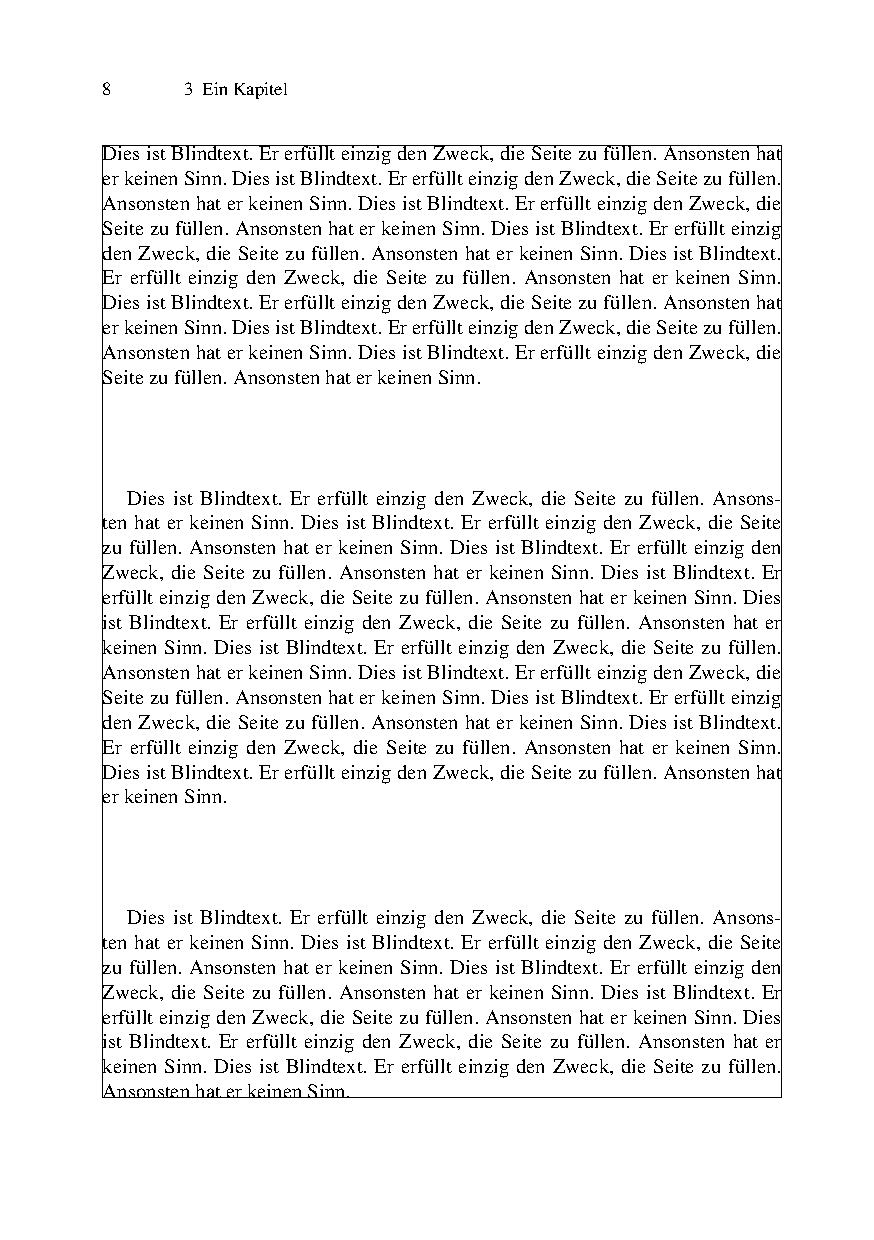
\includegraphics[width=0.24\linewidth,page=1]{bilder/seiten/umbruch1}}%
    \fbox{%
      \includegraphics[width=0.24\linewidth,page=2]{bilder/seiten/umbruch1}}%
    \label{fig:umbruch1a}%
  }%
  \hfill
  \subfigure[Verbesserter Seitenumbruch durch tempor�re Ver�nderung
  des Satzspiegels]{%
    \fbox{%
      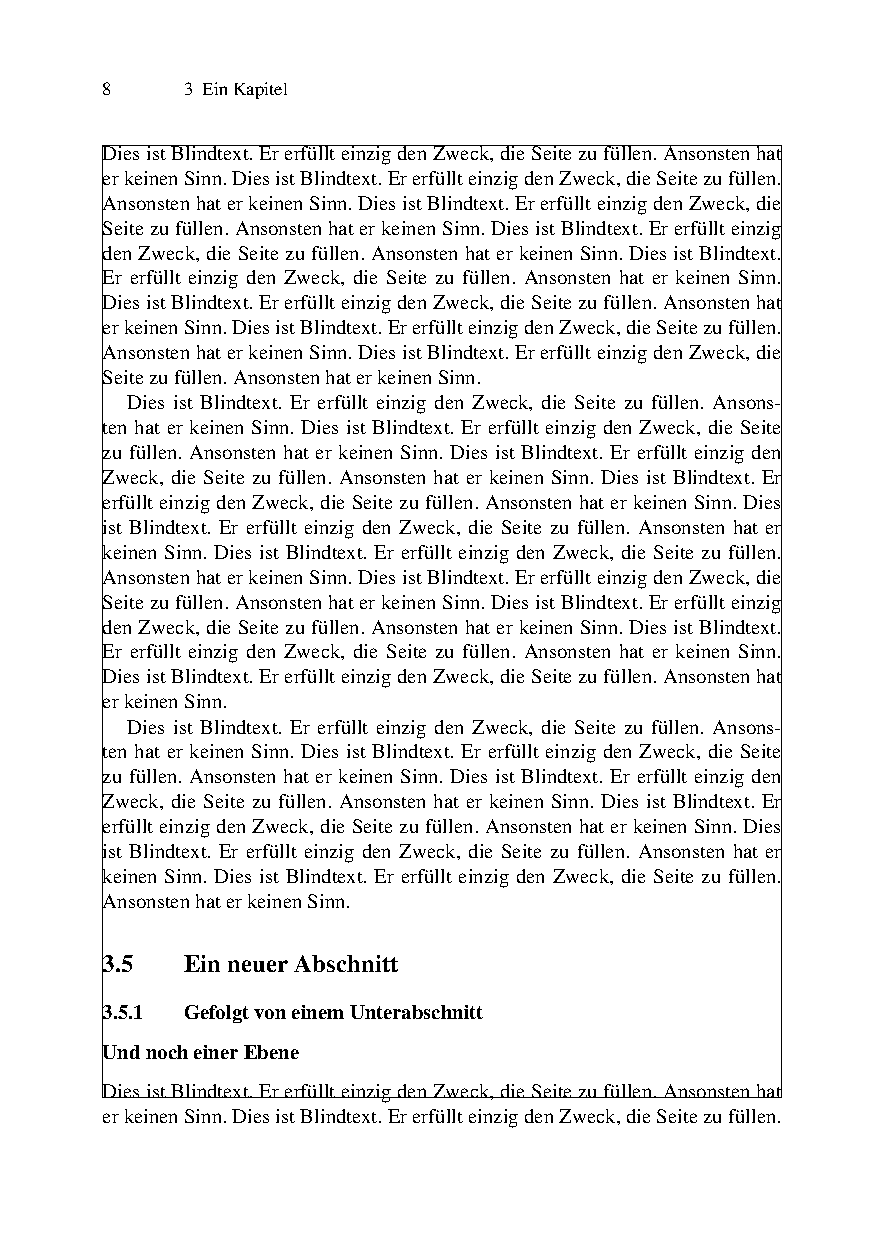
\includegraphics[width=0.24\linewidth,page=1]{bilder/seiten/umbruch1a}}%
    \fbox{%
      \includegraphics[width=0.24\linewidth,page=2]{bilder/seiten/umbruch1a}}%
    \label{fig:umbruch1b}%
  }%
  \caption[Verbesserung des Layouts durch manuelle Eingriffe in den
  Umbruch]{Verbesserung des Layouts durch manuelle Eingriffe in den
    Umbruch.
  Zur Verdeutlichung wird der normale Satzspiegel durch den
  eingezeichneten Kasten markiert.}%
\end{figure}

Wenn nun der Satzspiegel auf der Doppelseite jeweils um eine Zeile
vergr��ert wird, passen die Abschnitts�berschriften noch auf die erste
Seite, so dass diese wieder vern�nftig gef�llt ist.
Es ist wichtig, immer ein Doppelseitenpaar (also eine gerade Seite
gefolgt von einer ungeraden) um das gleiche Ma� zu ver�ndern,
um auf einer Doppelseite einen einheitlichen unteren Satzspiegel zu
erhalten.

Bild~\ref{fig:umbruch2} zeigt einen anderen Fall.
%
\begin{figure}
  \centering
  \fboxsep0mm%
  \subfigure[Unsch�ner Seitenumbruch durch eine Fu�note]{%
    \fbox{%
      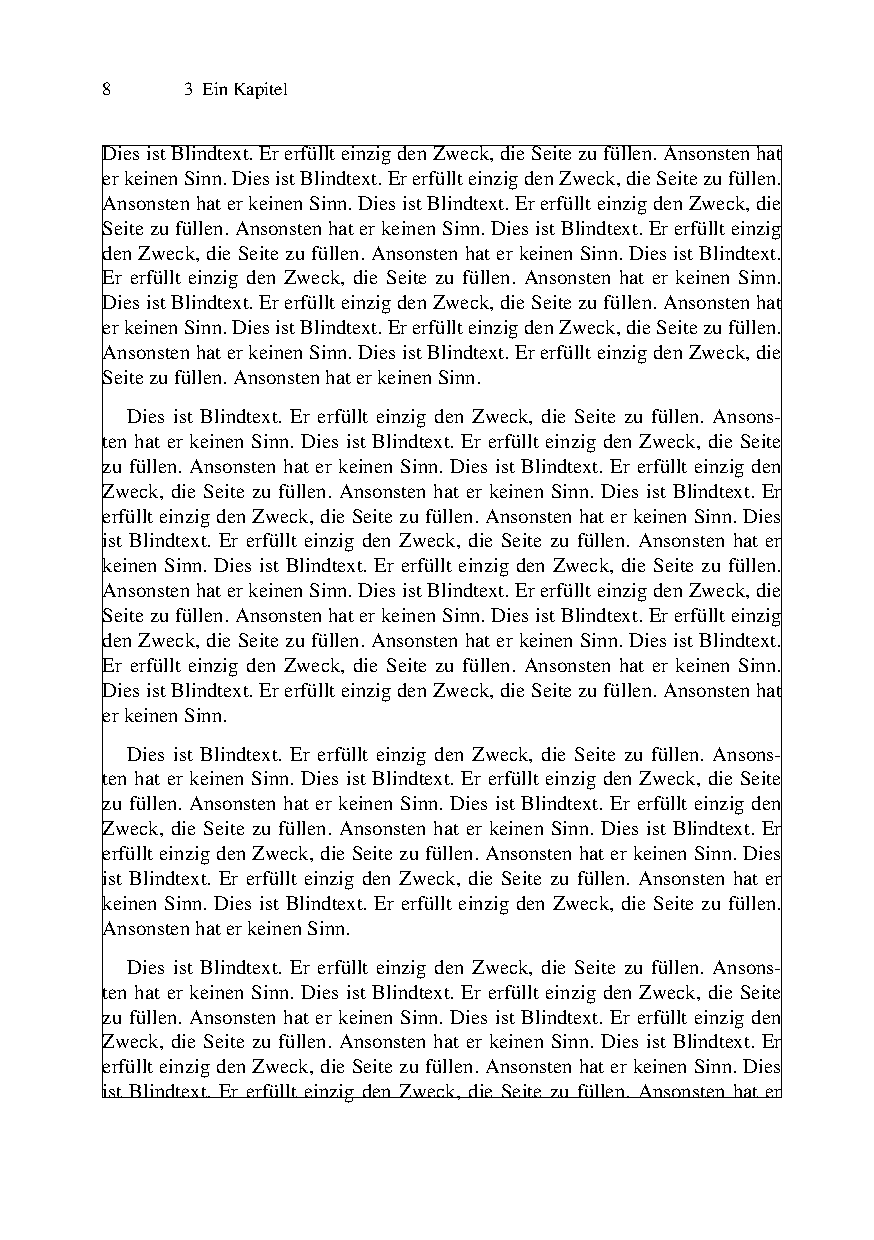
\includegraphics[width=0.24\linewidth,page=1]{bilder/seiten/umbruch2}}%
    \fbox{%
      \includegraphics[width=0.24\linewidth,page=2]{bilder/seiten/umbruch2}}%
    \label{fig:umbruch2a}%
  }%
  \hfill
  \subfigure[Verbesserter Seitenumbruch durch tempor�re Ver�nderung
  des Satzspiegels]{%
    \fbox{%
      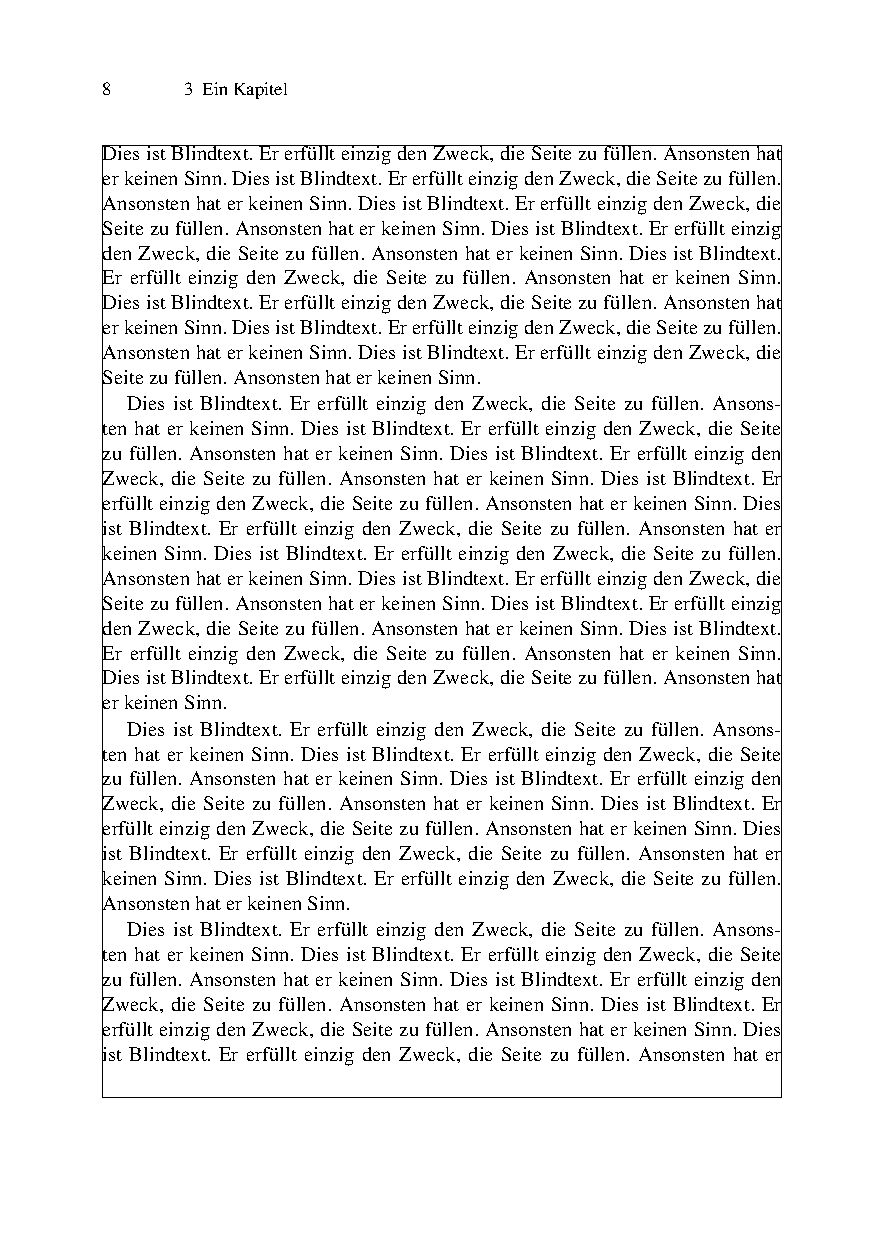
\includegraphics[width=0.24\linewidth,page=1]{bilder/seiten/umbruch2a}}%
    \fbox{%
      \includegraphics[width=0.24\linewidth,page=2]{bilder/seiten/umbruch2a}}%
    \label{fig:umbruch2b}%
  }%
  \caption[Verbesserung des Layouts durch manuelle Eingriffe in den
  Umbruch]{Verbesserung des Layouts durch manuelle Eingriffe in den
    Umbruch.
    Zur Verdeutlichung wird der normale Satzspiegel durch den
    eingezeichneten Kasten markiert.}%
  \label{fig:umbruch2}%
\end{figure}%
%
Die Fu�note m�sste eigentlich in der letzten Zeile der ersten Seite
ihre Markierung haben.
Dann w�rde allerdings der Fu�notentext auch auf diese Seite
geschrieben werden, wurdurch die Zeile mit der Fu�notenmarkierung auf
die n�chste Seite rutschen w�rde.
Dadurch rutscht aber auch die Fu�note selbst auf die n�chste Seite,
wodurch auf der ersten Seite wieder Platz f�r die Zeile mit der
Fu�notenmarkierung w�re.
Um diese Zwickm�hle zu umgehen, wird diese Zeile auf die n�chste Zeile
gezogen und die erste Seite gestreckt.
Hier ist es zweckm��ig, beide Seiten etwas zu verkleinern, um das
Strecken zu verhindern (Bild~\ref{fig:umbruch2b}).

H�ufig ist es gar nicht notwendig, in den Satzspiegel einzugreifen.
Beispielsweise kann es ausreichen, einen Satz geringf�gig
umzuformulieren, eine Abk�rzung auszuschreiben oder einen Begriff
abzuk�rzen, um einen Absatz um eine Zeile zu verl�ngern oder zu
verk�rzen und so unsch�ne Umbr�che zu verhindern.
Auch eine geringf�gige Vergr��erung oder Verkleinerung von Abbildungen
kann unsch�ne Umbr�che vermeiden.

Unsch�ne Umbr�che zeigen sich in der Log"=Datei durch Eintr�ge wie dem
folgenden:
\par\noindent
\begin{verbatim}[\small]
Underfull \vbox (badness 10000) has occurred while \output is active []

 [8] [9]
\end{verbatim}
\par\noindent
Die Zeile sagt, dass eine Seite durch Strecken der Abs�tze gef�llt
werden musste. 
Der Wert \verb|badness| zeigt an, wie "`schlimm"' das
Auseinanderziehen sein musste.
Der hier gezeigte Wert \np{10000} stellt das Maximum ("`unendlich"')
an.
Wenn die \emph{badness} kleine Werte im Bereich bis ca.\ \np{1500}
hat, kann die Seite noch ohne Ver�nderung akzeptabel sein.
Auf jeden Fall sollten Seiten mit dieser Warnung immer angeschaut
und im Einzelfall entschieden werden, ob eingegriffen werden
muss.
Das Umbruchproblem ist im Normalfall auf der Seite mit der Seitenzahl
entstanden, das der Warnung folgt.
Hier also auf Seite~8.

Es gibt auch weitere F�lle, die zwar nicht zu einem Auseinanderziehen
von Abs�tzen f�hren, aber dennoch verhindert werden sollten.
So kann es zum Beispiel passieren, dass die letzte Zeile eines
Abschnitts einsam auf der Folgeseite steht (sog.\ "`Hurenkind"'), wie
in Bild~\ref{fig:umbruch3} gezeigt.
%
\begin{figure}
  \centering
  \fboxsep0mm%
  \subfigure[Einzelne Zeile auf der Folgeseite]{%
    \fbox{%
      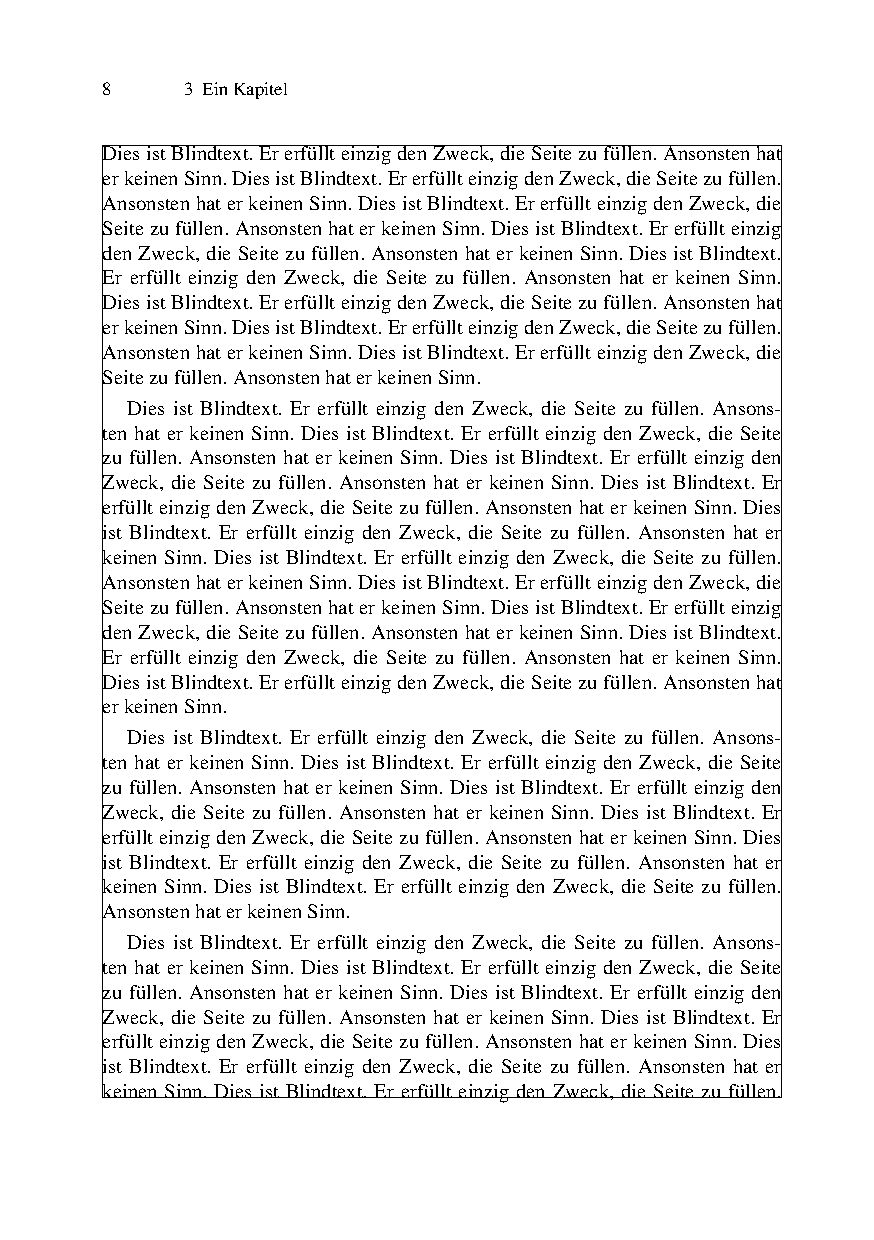
\includegraphics[width=0.24\linewidth,page=1]{bilder/seiten/umbruch3}}%
    \fbox{%
      \includegraphics[width=0.24\linewidth,page=2]{bilder/seiten/umbruch3}}%
    \label{fig:umbruch3a}%
  }%
  \hfill
  \subfigure[Problem behoben durch vergr��erten Satzspiegel]{%
    \fbox{%
      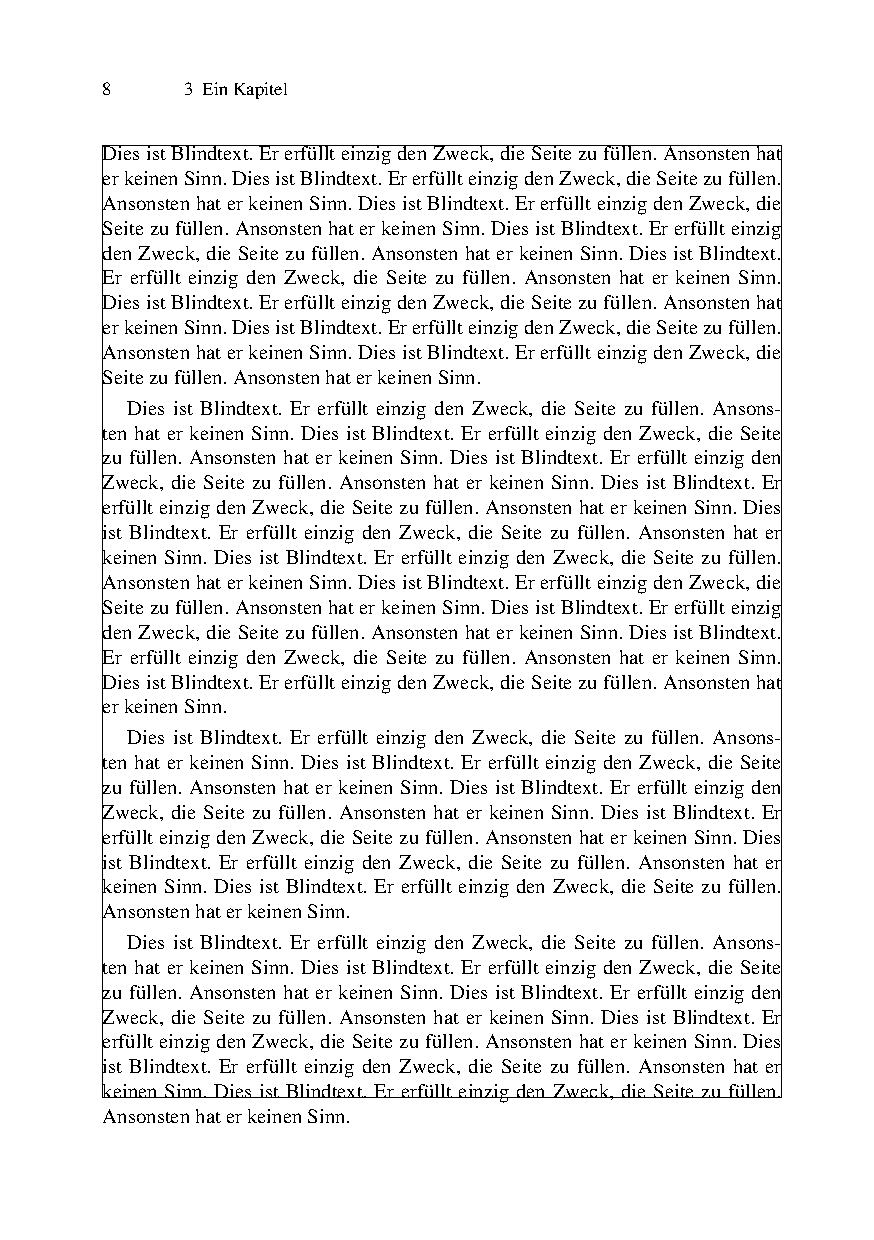
\includegraphics[width=0.24\linewidth,page=1]{bilder/seiten/umbruch3a}}%
    \fbox{%
      \includegraphics[width=0.24\linewidth,page=2]{bilder/seiten/umbruch3a}}%
    \label{fig:umbruch3b}%
  }%
  \caption[Verbesserung des Layouts durch manuelle Eingriffe in den
  Umbruch]{Verbesserung des Layouts durch manuelle Eingriffe in den
    Umbruch.
    Zur Verdeutlichung wird der normale Satzspiegel durch den
    eingezeichneten Kasten markiert.}%
  \label{fig:umbruch3}%
\end{figure}%
%
Hier kann zum Beispiel wieder eine Vergr��erung des Satzspiegels
helfen.

Auch Fu�noten selbst k�nnen Probleme bereiten. 
Unter Umst�nden kann es dazu kommen, dass Fu�noten �ber zwei Seiten
umbrochen werden.
H�ufig stellt dies kein Problem dar, beispielsweise wenn der erste
Teil der Fu�note auf einer geraden, der zweite Teil auf einer
ungeraden Seite ist und nicht nur wenige Worte umbrochen wurden.
Manchmal sind die Umbr�che jedoch auch sehr ungeschickt, so dass sie
vermieden werden sollten.
Da \LaTeX\ nicht entscheiden kann, wann ein Umbruch in einer Fu�note
akzeptabel ist, wird nur eine Warnung ins Logfile ausgegeben:
\par\noindent
\begin{verbatim}[\small]
Package fnbreak Warning: Footnote 1 has been split over different pages:
(fnbreak)                page 8 to page 9.
\end{verbatim}
\par\noindent
Hier sollten die Seiten~8 und 9 angeschaut werden und entschieden
werden, ob die Fu�note ver�ndert werden muss oder nicht.

Ein Vergr��ern bzw.\ Verkleinern des Satzspiegels geschieht durch
Einf�gen des Befehls
\begin{verbatim}[\small\makeescape\|\makebgroup\[\makeegroup\]]
\enlargethispage{|meta[Ma�]}
\end{verbatim}
auf beide Seiten, die in der Gr��e ver�ndert werden sollen.
Dabei sollte meist ein Vielfaches des Zeilenabstandes verwendet
werden, also z.\,B.
\begin{verbatim}[\small]
\enlargethispage{-2\baselineskip}
\end{verbatim}
Es sollte aber darauf geachtet werden, dass die Ver�nderungen gering
bleiben, besonders beim Vergr��ern des Satzspiegels.
Dabei stellen \verb|1\baselineskip| und \verb|-2\baselineskip| die
Grenzen dar, die nicht �berschritten werden sollten.

Dieser Feinschliff muss als allerletzte Arbeit erfolgen, nach dem
letzten Korrekturlesen, da auch kleine �nderungen am Dokument gro�e
�nderungen bei diesen Umbruchproblemen bewirken k�nnen.
Au�erdem m�ssen die Arbeiten von vorne nach hinten durchgef�hrt werden
und nach jeder �nderung neu �bersetzt werden, da eine �nderung vorne
unweigerlich �nderungen weiter hinten im Dokument nach sich zieht.

Die Arbeit ist zeitaufw�ndig und erfordert einiges
Fingerspitzengef�hl, um gute Ergebnisse erzielen zu k�nnen.
Es kann sinnvoll sein, dass diese Arbeiten von einer Person
durchgef�hrt werden, die hiermit Erfahrung besitzt.
Sprechen Sie dar�ber mit dem zust�ndigen Lektor beim Teubner Verlag.

% ===================================================================

%%% Local Variables: 
%%% mode: latex
%%% TeX-master: "bgteubner"
%%% End: 


% ===================================================================
% Anhang:
\appendix
% ===================================================================

\section{Mise en place du package}\label{MP}
%==================================


	\subsection{Installation}\label{installation}
	%--------------------------

		Le package s'installe comme n'importe quel autre.
		Apr�s l'avoir t�l�charg�, copier le :
		\begin{itemize}
			\item soit dans le dossier du document que vous �tes en train de r�diger (c'est une m�thode facile, mais il ne sera valable que pour ce document-l�)
			\item soit dans un des dossiers par d�faut de latex.
				L'emplacement de ces dossiers d�pendent du logiciel et du syst�me d'exploitation utilis� (Windows, Mac, Linux, etc.).
		\end{itemize}

	\subsection{Packages requis}\label{packages}
	%-----------------------------------

		Pour que le package fonctionne, vous devez d�j� avoir les packages suivants d'install�s :
		\begin{itemize}
			\item \href{http://sourceforge.net/projects/pgf/}{\textbf{TikZ}} : Package de dessin vectoriel sur lequel repose le diagramme fast,
			\item \href{http://www.ctan.org/pkg/ifthen}{\textbf{ifthen}} : Package permettant une compilation � choix multiple,
			\item \href{http://www.ctan.org/pkg/relsize}{\textbf{relsize}} : Package permettant de g�rer les longueurs relatives (em, ...)
			\item \href{http://tug.ctan.org/tex-archive/macros/latex/contrib/xargs}{\textbf{xarg}} : Package permettant de cr�er des commandes � plusieurs arguments optionnels.
		\end{itemize}

	\subsection{Appel du package ``fast-diagram.sty''}\label{appel}
	%-------------------------------

		L'appel du package se fait simplement en �crivant dans l'ent�te du document :
%#########################
\begin{code}
\usepackage{fast-diagram}
\end{code}
%########################
		Afin d'�viter d'�ventuels conflits entre packages, toutes les commandes utilis�es ici sont pr�c�d�es du pr�fixe {\color{blue}\verb'fast'}
		(par exemple {\color{blue}\verb'\fastFT'} pour d�signer la fonction technique \verb'FT').
		Pour la mise en place de raccourcis, l'option {\color{blue}\verb'[raccourcis]'} peut �tre apport�e dans le package de la mani�re suivante :
%#########################
\begin{code}
\usepackage[raccourcis]{fast-diagram}
\end{code}
%########################
		Les raccourcis seront d�velopp�s plus tard.
%
% bgteubner class bundle
%
% tex_aufruf.tex
% Copyright 2003--2012 Harald Harders
%
% This program may be distributed and/or modified under the
% conditions of the LaTeX Project Public License, either version 1.3
% of this license or (at your opinion) any later version.
% The latest version of this license is in
%    http://www.latex-project.org/lppl.txt
% and version 1.3 or later is part of all distributions of LaTeX
% version 1999/12/01 or later.
%
% This program consists of all files listed in manifest.txt.
% ===================================================================
%\documentclass[ngerman]{...}
% ===================================================================
\chapter{Aufruf der Programme}%
\index{Programmaufruf}%

Da der Teubner Verlag \acro{PDF}"=Dateien entgegennimmt und die
besten Resultate durch die Verwendung von \pdfLaTeX\ erzielt werden
konnten, wird vorgeschrieben, \pdfLaTeX\ zu verwenden.

Nehmen wir an, dass die Hauptdatei des Dokuments \verb|buch.tex| hei�t.
Das Programm \pdfLaTeX\ wird mit
\begin{verbatim}[\small]
pdflatex buch
\end{verbatim}
\index{Programmaufruf!pdfLaTeX@\pdfLaTeX}%
\index{pdfLaTeX@\pdfLaTeX!Programmaufruf}%
aufgerufen.
Um im Stichwortverzeichnis das richtige Layout zu erhalten, muss
Makeindex folgenderma�en aufgerufen werden:
\begin{verbatim}[\small]
makeindex -c -g -s bgteubner.ist buch
\end{verbatim}
\index{Programmaufruf!makeindex@\texttt{makeindex}}%
\index{makeindex@\texttt{makeindex}!Programmaufruf}%
Au�erdem muss das Literaturverzeichnis, das mit \BibTeX\
erstellt werden soll, mit
\begin{verbatim}[\small]
bibtex buch
\end{verbatim}
\index{Programmaufruf!bibtex@\texttt{bibtex}}%
\index{bibtex@\texttt{bibtex}!Programmaufruf}%
erzeugt werden.

\begingroup
\feinschliff{\def\Typ{\meta{T}}}{\def\Typ{\meta{Typ}}}%
  {\def\Typ{\meta{T}}}{\def\Typ{\meta{T}}}%
Glossar�hnliche Umgebungen werden ebenfalls mit dem Programm
\verb|makeindex| erzeugt. 
F�r einen Glossartypen \Typ\ lautet der Aufruf:
\begin{verbatim}[\small\makeescape\|\makebgroup\[\makeegroup\]]
makeindex -c -g -s bgteuglo.ist -t buch.glg|Typ -o buch.gls|Typ buch.glo|Typ
\end{verbatim}
\endgroup
Statt \verb|bgteuglo.ist| kann auch \verb|bgteuglochar.ist| verwendet
werden, wenn der Glossar �berschriften f�r die Buchstaben erhalten
soll.
Beispielsweise f�r einen mit dem Befehl \cs{makeglossary\marg{cmd}}
eingerichteten Glossar:
\begin{verbatim}[\small\makeescape\|\makebgroup\[\makeegroup\]]
makeindex -c -g -s bgteuglo.ist -t buch.glgcmd -o buch.glscmd buch.glocmd
\end{verbatim}

Um auf jeden Fall ein richtig formatiertes Buch mit korrekten
Querverweisen zu erhalten, muss \pdfLaTeX\ mehrmals aufgerufen werden.
Folgende Aufruf"|folge ist denkbar:
\begin{verbatim}[\small]
pdflatex buch
pdflatex buch
makeindex -c -g -s bgteuglo.ist -t buch.glgcmd -o buch.glscmd buch.glocmd
bibtex buch
pdflatex buch
pdflatex buch
makeindex -c -g -s bgteubner.ist buch
pdflatex buch
\end{verbatim}
In seltenen F�llen kann sogar noch h�ufigeres �bersetzen notwendig
sein.

Auch wenn in den meisten F�llen diese Prozedur �bertrieben ist,
sollte man sie zur Erstellung der endg�ltigen Datei, die an die
Druckerei weitergegeben wird, einmal vollst�ndig durchf�hren.
W�hrend der Erstellung des Buches ist das nat�rlich nicht notwendig.


% ===================================================================

%%% Local Variables: 
%%% mode: latex
%%% TeX-master: "bgteubner"
%%% End: 

%
% bgteubner class bundle
%
% checkliste.tex
% Copyright 2003--2012 Harald Harders
%
% This program may be distributed and/or modified under the
% conditions of the LaTeX Project Public License, either version 1.3
% of this license or (at your opinion) any later version.
% The latest version of this license is in
%    http://www.latex-project.org/lppl.txt
% and version 1.3 or later is part of all distributions of LaTeX
% version 1999/12/01 or later.
%
% This program consists of all files listed in manifest.txt.
% ===================================================================
\chapter{Checkliste}%
\index{Checkliste|textbf}%
\label{sec:checkliste}%

An dieser Stelle wird eine Checkliste angeboten, die man durcharbeiten
sollte, bevor man dem Verlag eine endg�ltige Version seines
Buches zukommen l�sst.
%
\begin{enumerate}
\item Sind so wenig zus�tzliche Pakete geladen wie m�glich?
  (Es m�ssen weniger Pakete geladen werden als bei den meisten anderen
  Dokumentklassen.
  Beispielsweise m�ssen weder \texttt{babel} noch \texttt{fontenc}
  zus�tzlich geladen werden.)
\item L�uft der �bersetzungslauf fehlerfrei durch?\footnote{Gerade
    unter Windows findet man manchmal Installationen, die auch an
    Fehlern die �bersetzung nicht unterbrechen.
    Schauen Sie auf jeden Fall in die Log"=Datei, ob keine Fehler
    aufgetreten sind.}
\item Wurde im gesamten Werk, inklusive aller Vorworte, einheitlich
  entweder die neue oder die alte Rechtschreibung verwendet und auch
  in der \verb|\documentclass|"=Zeile die entsprechende Sprache als
  letztes angegeben?
  Die neue Rechtschreibung ist vorzuziehen.
\item Entsprechen die Abs�tze vor und nach abgesetzten Formeln der
  inhaltlichen Gliederung? Keine unn�tigen Abs�tze!
\item Sind durch Flie�umgebungen keine unn�tigen Abs�tze oder
  Leerzeichen entstanden?
\item Sind alle Angaben zum Buch (Autoren, Titel etc.) korrekt?
\item Entsprechen alle Datumsangaben (z.\,B.\ im Vorwort) dem
  Erscheinungsjahr und "~monat?
\item Wurde in allen F�llen zwischen Zahlen im Text"= und Mathemodus
  unterschieden?
\item Wurden alle Formelzeichen auch wirklich im mathematischen Modus
  gesetzt?
\item Haben alle Zahlen Kommata statt Punkte?
\item Tabellen haben �berschriften, keine Unterschriften!
\item Ist das Stichwortverzeichnis erstellt und nicht zu knapp
  gehalten?
\item L�uft die Erzeugung des Literaturverzeichnisses mit \BibTeX\
  fehlerfrei und ohne Warnung ab (siehe Log"=Datei mit der Endung
  \verb|.blg|)?
\item Sind alle fehlenden Referenzen und doppelten Labels behoben?
\item Wurde bei den letzten �bersetzungsl�ufen ohne die Option
  \verb|draft| gearbeitet?
\item\label{enum:uebersetzen}
  Wurde oft genug �bersetzt, so dass alle Referenzen und
  Seitenzahlen in den entsprechenden Verzeichnissen stimmen?
\item Wurde der Index sp�t genug neu erzeugt, so dass auch dort alle
  Seitenzahlen stimmen?
\item\label{enum:overfull}
  Sind alle "`Overfull \textbackslash hbox"' (schwarze Balken,
  falls mit der Option \verb|draft| �bersetzt) behoben?
\item Wenn Sie lange Tabellen mit der \env{longtable}"=Umgebung
  verwenden: Sind alle doppelten Linien an Seitenumbr�chen beseitigt
  worden (vgl.\ Abschnitt~\ref{sec:tex:tabellen}), und ist die
  Reihenfolge der Tabellen korrekt?
\item\label{enum:feinschliff}
  Wurde der Feinschliff entsprechend
  Abschnitt~\ref{sec:tex_feinschliff} zur Vermeidung unsch�ner
  Umbr�che durchgef�hrt (u.\,A.\ Beheben von "`Underfull
  \textbackslash vbox"')? 
\item\label{enum:indexwiderspruch}
  Wurde darauf geachtet, dass sich keine widerspr�chlichen
  Indexangaben entsprechend Abschnitt~\ref{sec:tex_index_doppelt}
  ergeben haben?
\item Wurde die endg�ltige \acro{PDF}"=Datei ausgedruckt und
  sorgf�ltig auf Fehler hin kontrolliert?
  Wenn noch Fehler gefunden werden, m�ssen wahrscheinlich die
  Punkte~\ref{enum:uebersetzen} bis \ref{enum:indexwiderspruch}
  wiederholt werden.
\end{enumerate}

Einige dieser Fragen lassen sich am einfachsten dadurch beantworten,
dass man sich die Log"=Datei von \pdfLaTeX\ ansieht.
Beispielsweise werden fehlende und doppelte Verweise, sowie "`Overfull
\textbackslash hbox"' und "`Underfull \textbackslash vbox"' dort genannt.

% ===================================================================
%%% Local Variables: 
%%% mode: latex
%%% TeX-master: "bgteubner"
%%% End: 

%
% bgteubner class bundle
%
% optionen-advanced.tex
% Copyright 2003--2012 Harald Harders
%
% This program may be distributed and/or modified under the
% conditions of the LaTeX Project Public License, either version 1.3
% of this license or (at your opinion) any later version.
% The latest version of this license is in
%    http://www.latex-project.org/lppl.txt
% and version 1.3 or later is part of all distributions of LaTeX
% version 1999/12/01 or later.
%
% This program consists of all files listed in manifest.txt.
% ===================================================================
\chapter{Anmerkungen f�r versierte Nutzer}%
\label{chap:optionen-advanced}%

Da der normale Anwender die in diesem Anhang beschriebenen Dinge
normalerweise nicht ben�tigt, sind sie kleiner gedruckt.

\section{Erweiterte Klassenoptionen}
\begin{advanced}
  \setkomafont{caption}{\rmfamily\footnotesize\RaggedRight}%
  \setkomafont{float}{\normalfont\normalcolor\footnotesize}%
  \renewcommand{\subcapsize}{\footnotesize}%
  %
  Gegen�ber den in Abschnitt~\ref{sec:tex:aufbau} beschriebenen
  Klassenoptionen unterst�tzt \verb|bgteubner| einige weitere
  Optionen, die normalerweise nicht verwendet werden sollen. 
  In den meisten F�llen f�hren sie zu einem Layout, das inkonsistent
  mit den Vorgaben des Verlags ist.
  In Tabelle~\ref{tab:klassenoptionen-advanced} sind diese Optionen
  ohne ausf�hrliche Erkl�rungen zusammengefasst.
  %
  \begin{table}%
    \centering
    \def\default{{\rmfamily*}}%
    \caption{Selten ben�tigte Klassenoptionen der Klasse \texttt{bgteubner}.
      Defaultm��ig aktivierte Optionen sind mit einem \default\
      gekennzeichnet.}%
    \label{tab:klassenoptionen-advanced}%
    \begin{tabular}{>{\ttfamily}ll}
      \toprule
      \rmfamily Option& Erkl�rung \\
      \midrule
      headingoutside\default & Lebender Kolumnentitel au�en \\
      headinginside& Lebender Kolumnentitel innen \\
      \midrule
      tocindent\default & Inhaltsverzeichnis mit Einr�ckung setzen \\
      tocleft& Inhaltsverzeichnis linksb�ndig \\
      \midrule
      springervieweg\default & Verlagsname Springer Vieweg auf der
      Titelseite \\
      viewegteubner & Verlagsname Vieweg+Teubner auf der Titelseite \\
      bgteubner & Verlagsname B.\,G.\ Teubner auf der Titelseite \\
%      \midrule
%      epsfigures& Setzt Bilder auch bei normalem \LaTeX\ (dvi"=Ausgabe) \\
      \bottomrule
    \end{tabular}
  \end{table}%
\end{advanced}

                                
\section{\acro{PDF}"=Informationen f�r den Verlag}%
\label{sec:pdf-informationen}%
\begin{advanced}
  \setkomafont{caption}{\rmfamily\footnotesize\RaggedRight}%
  \setkomafont{float}{\normalfont\normalcolor\small}%
  \renewcommand{\subcapsize}{\footnotesize}%
  %
  Bei der Erstellung des Dokuments sollen die Autoren einige Felder
  bez�glich des Titels und der Autoren ausf�llen (Befehle \cs{title},
  \cs{subtitle}, \cs{author}, \cs{edition}).
  Diese werden in die Info"=Felder der \acro{PDF}"=Datei
  geschrieben, die im \emph{Acrobat Reader} abgerufen werden k�nnen
  (\emph{File -- Document Properties -- Summary}).
  Im Feld \emph{Title} erscheint der Titel.
  Das \emph{Subject}"=Feld wird f�r den Untertitel und die Auf"|lage
  zweckentfremdet.
  Die Autoren erscheinen im Feld \emph{Author}.
  Das Feld \emph{Keywords} wird zweckentfremdet f�r die Angabe der
  Anzahl der Abbildungen, Tabellen, Aufgaben, Beispiele usw.
  Hier kann der Lektor des Teubner Verlags immer die aktuelle Anzahl
  der entsprechenden Umgebungen ablesen, da diese f�r das Titelblatt
  notwendig ist.
  Es kann so nicht passieren, dass eine inkorrekte Zahl angegeben
  wird.

  Unter \emph{Creator} wird die Version der Dokumentklasse angegeben. 
  Dies ist in seltenen F�llen von Nutzen, um zu kontrollieren, ob eine
  eventuelle alte Version verwendet wurde.
  
  Das Erstellungsdatum im Feld \emph{Created} kann helfen, die neueste
  Version des Manuskriptes zu finden.
\end{advanced}


\section{Befehle f�r Fortgeschrittene}%
\label{sec:fortgeschrittene}%

\begin{advanced}
  Manchmal kann es n�tzlich sein zu pr�fen, ob eine bestimmte Version
  der Dokumentklasse verwendet wird.
  Dazu k�nnen Sie in der Dokumentpr�ambel den Befehl
\begin{verbatim}[\footnotesize\makeescape\|\makebgroup\[\makeegroup\]]
\version|marg[Versionsnummer]
\end{verbatim}
  verwenden.

  M�chten Sie zum Beispiel pr�fen, ob Version 1.03 der Dokumentklasse
  verwendet wird, schreiben Sie
\begin{verbatim}[\footnotesize]
\version{1.03}
\end{verbatim}
  in die Pr�ambel.
  Stimmen die angegebene und die tats�chliche Versionsnummer nicht
  �berein, wird eine Warnung in die Log"=Datei geschrieben.
\end{advanced}


% ===================================================================

%%% Local Variables: 
%%% mode: latex
%%% TeX-master: "bgteubner"
%%% End: 


%
% bgteubner class bundle
%
% befehlsreferenz.tex
% Copyright 2003--2012 Harald Harders
%
% This program may be distributed and/or modified under the
% conditions of the LaTeX Project Public License, either version 1.3
% of this license or (at your opinion) any later version.
% The latest version of this license is in
%    http://www.latex-project.org/lppl.txt
% and version 1.3 or later is part of all distributions of LaTeX
% version 1999/12/01 or later.
%
% This program consists of all files listed in manifest.txt.
% ===================================================================
\glossarycmd{advanced@\cs{advanced}}{einger�ckter Textblock f�r weitergehende Dinge (\ref{sec:tex:saetze})}%
\glossarycmd{answer@\cs{answer}}{nummerierte L�sung (\ref{sec:tex:aufgaben})}%
\glossarycmd{answer*@\cs{answer*}}{unnummerierte L�sung (\ref{sec:tex:aufgaben})}%
\glossarycmd{author@\cs{author}}{Autoren (\ref{sec:tex:aufbau})}%
\glossarycmd{backmatter@\cs{backmatter}}{Schluss des Buchs (wird ignoriert)}%
\glossarycmd{bigskip@\cs{bigskip}}{Abschnitt mit gro�em Abstand (\ref{sec:tex:teile})}%
\glossarycmd{cases*@\env{cases*}}{Fallunterscheidung mit schlie�ender Klammer (\ref{sec:tex:mathematik})}%
\glossarycmd{d@\cs{d}}{Mathematik: Differentialoperator $\d$, Text: Punkt unter dem folgenden Zeichen \d a (\ref{sec:tex:mathematik})}%
\glossarycmd{D@\cs{D}}{Differenzoperator $\D$ (\ref{sec:tex:mathematik})}%
\glossarycmd{dedication@\cs{dedication}}{Widmung (\ref{sec:tex:aufbau})}%
\glossarycmd{e@\cs{e}}{eulersche Zahl (\ref{sec:tex:mathematik})}%
\glossarycmd{edition@\cs{edition}}{Auf"|lage des Buchs (\ref{sec:tex:aufbau})}%
\glossarycmd{engl@\cs{engl}}{fremdsprachiger Begriff
  (\ref{sec:tex:auszeichnungen})}% 
\glossarycmd{equivalent@\cs{equivalent}}{Entspricht"=Zeichen:
  $\equivalent$ (\ref{sec:tex:mathematik})}%
\glossarycmd{exercise@\env{exercise}}{nummerierte Aufgabe (\ref{sec:tex:aufgaben})}%
\glossarycmd{exercise*@\env{exercise*}}{unnummerierte Aufgabe (\ref{sec:tex:aufgaben})}%
\glossarycmd{frontmatter@\cs{frontmatter}}{Titelei des Buchs (\ref{sec:tex:aufbau})}%
\glossarycmd{glossary@\cs{glossary\meta{Name}}}{definiert einen Eintrag f�r einen Glossar des Typs \meta{Name} (\ref{sec:tex:glossary})}%
\glossarycmd{glossaryname@\cs{glossary\meta{Name}name}}{definiert den �berschriftsnamen f�r einen Glossar des Typs \meta{Name} (\ref{sec:tex:glossary})}%
\glossarycmd{glossarypreamble@\cs{glossary\meta{Name}preamble}}{definiert die Pr�ambel eines Glossars des Typs \meta{Name} (\ref{sec:tex:glossary})}%
\glossarycmd{grad@\cs{grad}}{Gradient (\ref{sec:tex:mathematik})}%
\glossarycmd{important@\env{important}}{grau hinterlegte Box (mit Text
  beginnend) (\ref{sec:tex:important})}%
\glossarycmd{important*@\env{important*}}{grau hinterlegte Box (mit
  einer abgesetzten Formel beginnend) (\ref{sec:tex:important})}%
\glossarycmd{longimportant@\env{longimportant}}{lange grau hinterlegte
  Box (mit Text beginnend) (\ref{sec:tex:important})}%
\glossarycmd{longimportant*@\env{longimportant*}}{lange grau hinterlegte
  Box (\ref{sec:tex:important})}%
\glossarycmd{listofexamples@\cs{listofexamples}}{Beispielverzeichnis
  (\ref{sec:tex:beispielverzeichnis})}%
\glossarycmd{listofexercises@\cs{listofexercises}}{Aufgabenverzeichnis
  (\ref{sec:tex:beispielverzeichnis})}%
\glossarycmd{listofdefinitions@\cs{listofdefinitions}}{Verzeichnis der
  Definitionen (\ref{sec:tex:beispielverzeichnis})}%
\glossarycmd{listofproofs@\cs{listofproofs}}{Verzeichnis der
  Beweise (\ref{sec:tex:beispielverzeichnis})}%
\glossarycmd{listoftheorems@\cs{listoftheorems}}{Verzeichnis der Umgebungen einer Theoremart (\ref{sec:tex:saetze})}%
\glossarycmd{listoffigures@\cs{listoffigures}}{Abbildungsverzeichnis
  (\ref{sec:tex:abbildungsverzeichnis})}%
\glossarycmd{listoftables@\cs{listoftables}}{Tabellenverzeichnis
  (\ref{sec:tex:abbildungsverzeichnis})}%
\glossarycmd{mainmatter@\cs{mainmatter}}{Hauptteil des Buchs (\ref{sec:tex:aufbau})}%
\glossarycmd{makeglossary@\cs{makeglossary}}{definiert einen neuen Typ an glossar�hnlicher Liste wie z.\,B.\ dieser Befehlsreferenz (\ref{sec:tex:glossary})}%
\glossarycmd{matr@\cs{matr}}{Matrix (\ref{sec:tex:mathematik})}%
\glossarycmd{medskip@\cs{medskip}}{Abschnitt mit mittlerem Abstand (\ref{sec:tex:teile})}%
\glossarycmd{new@\cs{new}}{neu eingef�hrter Begriff
  (\ref{sec:tex:auszeichnungen})}%
\glossarycmd{newtheorem@\cs{newtheorem}}{Einrichten einer neuen theoremartigen Umgebung (\ref{sec:tex:saetze})}%
\glossarycmd{nomathindent@\env{nomathindent}}{Einzug von abgesetzten
  Gleichungen reduzieren (\ref{sec:tex:mathematik})}%
\glossarycmd{person@\cs{person}}{Personenname
  (\ref{sec:tex:auszeichnungen})}%
\glossarycmd{printglossary@\cs{printglossary\meta{Name}}}{Setzen eines Glossars des Typs \meta{Name} (\ref{sec:tex:glossary})}%
\glossarycmd{smallskip@\cs{smallskip}}{Abschnitt mit kleinem Abstand (\ref{sec:tex:teile})}%
\glossarycmd{subanswer@\env{subanswer}}{nummerierte L�sung (\ref{sec:tex:aufgaben})}%
\glossarycmd{subanswer*@\env{subanswer*}}{unnummerierte L�sung (\ref{sec:tex:aufgaben})}%
\glossarycmd{subexercise@\env{subexercise}}{Nummerierte Aufgabe (\ref{sec:tex:aufgaben})}%
\glossarycmd{subexercise*@\env{subexercise*}}{unnummerierte Aufgabe (\ref{sec:tex:aufgaben})}%
\glossarycmd{subtask@\env{subtask}}{Teilaufgaben (\ref{sec:tex:aufgaben})}%
\glossarycmd{subtaskref@\cs{subtaskref}}{Referenz auf eine Teilaufgabe (\ref{sec:tex:aufgaben})}%
\glossarycmd{subtitle@\cs{subtitle}}{Untertitel des Buchs (\ref{sec:tex:aufbau})}%
\glossarycmd{tensor@\cs{tensor}}{Tensor h�herer Stufe (\ref{sec:tex:mathematik})}%
\glossarycmd{theglossary@\env{theglossary}}{manuell eingegebener Glossar (\ref{sec:tex:glossary})}%
\glossarycmd{example@\env{example}}{nummieriertes, abgesetztes Beispiel
  (\ref{sec:tex:saetze})}%
\glossarycmd{example*@\env{example*}}{unnummeriertes, abgesetztes Beispiel (\ref{sec:tex:saetze})}%
\glossarycmd{definition@\env{definition}}{nummerierte, abgesetzte
  Definition (\ref{sec:tex:saetze})}% 
\glossarycmd{definition*@\env{definition*}}{unnummerierte, abgesetzte
  Definition (\ref{sec:tex:saetze})}% 
\glossarycmd{proof@\env{proof}}{nummerierte, abgesetzte
  Beweise (\ref{sec:tex:saetze})}% 
\glossarycmd{proof*@\env{proof*}}{unnummerierte, abgesetzte
  Beweise (\ref{sec:tex:saetze})}% 
\glossarycmd{qed@\cs{qed}}{rechtsb�ndiger schwarzer Kasten zum
  Abschluss eines Beweises (\ref{sec:tex:saetze})}% 
\glossarycmd{qedname@\cs{qedname}}{Text am Ende eines Beweises
  (\ref{sec:tex:saetze})}%
\glossarycmd{title@\cs{title}}{Titel des Buchs (\ref{sec:tex:aufbau})}%
\glossarycmd{tr@\cs{tr}}{Spur eines Tensors (\ref{sec:tex:mathematik})}%
\glossarycmd{signature@\cs{signature}}{Unterschrift der Autoren f�r ein Vorwort (\ref{sec:vorwort})}%
\glossarycmd{vec@\cs{vec}}{Vektor (\ref{sec:tex:mathematik})}%
\glossarycmd{acro@\cs{acro}}{druckt eine Abk�rzung aus
  Versalien etwas kleiner (\ref{sec:tex:acro})}%
\glossarycmd{version@\cs{version}}{pr�ft, ob die richtige Version von
  \texttt{bgteubner.cls} verwendet wird (\ref{sec:fortgeschrittene})}%
\glossarycmd{preface@\cs{preface}}{�berschrift f�r Vorworte (\ref{sec:vorwort})}%
\glossarycmd{f@\cs{f}}{im Index ein "`f"' an eine Seitenzahl h�ngen
  (\ref{sec:tex_index})}% 
\glossarycmd{ff@\cs{ff}}{im Index ein "`ff"' an eine Seitenzahl h�ngen
  (\ref{sec:tex_index})}% 
\glossarycmd{textbff@\cs{textbff}}{im Index ein "`f"' an eine fettgedruckte
  Seitenzahl h�ngen (\ref{sec:tex_index})}% 
\glossarycmd{textbfff@\cs{textbfff}}{im Index ein "`ff"' an eine fettgedruckte
  Seitenzahl h�ngen (\ref{sec:tex_index})}% 
\glossarycmd{subind@\cs{subind}}{Querverweis auf einen Unterpunkt im
  Index (\ref{sec:tex_index})}% 
\glossarycmd{index@\cs{index}}{Indexeintrag erzeugen
  (\ref{sec:tex_index})}%
\glossarycmd{theoremdelimiter@\env{theoremdelimiter}}{den Doppelpunkt
  nach der �berschrift einer theoremartigen Umgebung ersetzen
  (\ref{sec:tex:theorem})}%
\glossarycmd{settheoremmargin@\cs{settheoremmargin}}{Einr�ckung
  theoremartiger Umgebungen ver�ndern (\ref{sec:tex:theorem})}%
\glossarycmd{exercisedelimiter@\env{exercisedelimiter}}{den Doppelpunkt
  nach der �berschrift einer Aufgabe oder L�sung ersetzen
  (\ref{sec:tex:aufgaben})}%

% ===================================================================

%%% Local Variables: 
%%% mode: latex
%%% TeX-master: bgteubner.tex
%%% TeX-master: "bgteubner"
%%% End: 

%%
%% This is file `index.sty',
%% generated with the docstrip utility.
%%
%% The original source files were:
%%
%% index.dtx  (with options: `style')
%% 
%% IMPORTANT NOTICE:
%% 
%% For the copyright see the source file.
%% 
%% Any modified versions of this file must be renamed
%% with new filenames distinct from index.sty.
%% 
%% For distribution of the original source see the terms
%% for copying and modification in the file index.dtx.
%% 
%% This generated file may be distributed as long as the
%% original source files, as listed above, are part of the
%% same distribution. (The sources need not necessarily be
%% in the same archive or directory.)
%% \CheckSum{755}
%% \CharacterTable
%%  {Upper-case    \A\B\C\D\E\F\G\H\I\J\K\L\M\N\O\P\Q\R\S\T\U\V\W\X\Y\Z
%%   Lower-case    \a\b\c\d\e\f\g\h\i\j\k\l\m\n\o\p\q\r\s\t\u\v\w\x\y\z
%%   Digits        \0\1\2\3\4\5\6\7\8\9
%%   Exclamation   \!     Double quote  \"     Hash (number) \#
%%   Dollar        \$     Percent       \%     Ampersand     \&
%%   Acute accent  \'     Left paren    \(     Right paren   \)
%%   Asterisk      \*     Plus          \+     Comma         \,
%%   Minus         \-     Point         \.     Solidus       \/
%%   Colon         \:     Semicolon     \;     Less than     \<
%%   Equals        \=     Greater than  \>     Question mark \?
%%   Commercial at \@     Left bracket  \[     Backslash     \\
%%   Right bracket \]     Circumflex    \^     Underscore    \_
%%   Grave accent  \`     Left brace    \{     Vertical bar  \|
%%   Right brace   \}     Tilde         \~}
\NeedsTeXFormat{LaTeX2e}[1995/06/01]

\ProvidesPackage{index}[2004/01/20 v4.2beta Improved index support (dmj)]
\def\disableindex#1{%
    \@for\@tempa:=#1\do{%
        \@namedef{disable@\@tempa}{}%
        \@ifundefined{tf@\@tempa}{}{%
            \PackageWarningNoLine{index}{It's too late to disable
                the `\@tempa' index;\MessageBreak
                \jobname.\@tempa\space has already
                been opened for output. You \MessageBreak
                should put the \string\disableindex\space command
                before\MessageBreak
                the declaration of the `\@tempa' index}%
        }%
    }%
}
\newif\if@newindex

\def\newindex{%
    \@tempswafalse
    \@ifnextchar[{\@tempswatrue\x@newindex}{\x@newindex[thepage]}%
}

\def\x@newindex[#1]{%
    \@ifstar {\@tempswafalse\y@newindex{#1}}
             {\y@newindex{#1}}%
}

\def\y@newindex#1#2{%
    \@ifundefined{idx@#2}%
        {\@newindextrue\def@index{#1}{#2}}%
        {%
            \@latexerr{Index type `\string#2' already defined}\@ehc
            \expandafter\@gobble\@gobbletwo
        }%
}

\def\renewindex{%
    \@tempswafalse
    \@ifnextchar[{\@tempswatrue\x@renewindex}{\x@renewindex[thepage]}%
}

\def\x@renewindex[#1]{%
    \@ifstar {\@tempswafalse\y@renewindex{#1}}
             {\y@renewindex{#1}}%
}

\def\y@renewindex#1#2{%
    \@ifundefined{idx@#2}%
        {%
            \@newindextrue
            \@latexerr{Index type `\string#2' not defined}\@ehc
        }%
        {\@newindexfalse}%
    \def@index{#1}{#2}%
}
\@onlypreamble\newindex
\@onlypreamble\renewindex
\@onlypreamble\disableindex
\def\def@index#1#2#3#4{%
    \@namedef{idx@#2}{#3:#4:#1}%
    \expandafter\let\csname if@immediate@#2\endcsname\if@tempswa
    \if@filesw
        \if@newindex
            \expandafter\newtoks\csname idxtitle@#2\endcsname
        \fi
        \@ifundefined{disable@#2}{%
            \if@newindex
                \expandafter\newwrite\csname tf@#2\endcsname
            \else
                \immediate\closeout\@nameuse{tf@#2}%
            \fi
            \immediate\openout\@nameuse{tf@#2}\jobname.#3 %
            \PackageInfo{index}{Writing index file \jobname.#3}%
        }
        {\PackageInfo{index}{Index `#2' disabled -- not opening
                      \jobname.#3}}%
    \fi
    \expandafter\csname idxtitle@#2\endcsname
}
\def\@second#1:#2:#3\@nil{#2}

\def\@third#1:#2:#3\@nil{#3}
\def\@nearverbatim{\expandafter\strip@prefix\meaning}
\edef\makeindex{%
    \noexpand\newindex{default}{idx}{ind}{\indexname}%
}
\newif\if@silentindex\@silentindextrue

\newif\if@addtoindex\@addtoindextrue

\newif\ifproofmode\proofmodefalse
\def\index{\protect\p@index}

\def\p@index{%
    \if@silentindex\@bsphack\fi
    \@ifstar{\@silentindexfalse\@xindex}{\@silentindextrue\@xindex}%
}

\def\@xindex{\@ifnextchar[{\@index}{\@index[default]}}
\def\@index[#1]{%
    \ifx\index\@gobble
        \@addtoindexfalse
    \fi
    \def\@tempf{%
        \begingroup
            \@sanitize
            \@@index{#1}%
    }%
    \if@addtoindex
        \@ifundefined{idx@#1}%
            {%
              \def\@tempf{%
                  \@latexerr{Index type `\string#1' undefined}%
                  \@ehc
                  \@silentindextrue
                  \@gobble
              }%
            }%
            {}%
    \fi
    \@tempf
}

\def\@@index#1#2{%
    \endgroup
    \if@addtoindex
        \if@filesw\@wrindex{#1}{#2}\fi
        \ifproofmode\@showidx{#2}\fi
    \fi
    \if@silentindex
        \expandafter\@esphack
    \else
        \@silentindextrue#2%
    \fi
}

\def\@wrindex#1#2{%
    \begingroup
        \def\@tempa{#2}%
        \edef\@tempb{\@nameuse{idx@#1}}%
        \edef\@tempb{\expandafter\@third\@tempb\@nil}%
        \csname if@immediate@#1\endcsname \else
            \expandafter\let\csname\@tempb\endcsname\relax
        \fi
        \edef\@tempa{%
           \write\@auxout{%
              \string\@writefile{#1}{%
                  \string\indexentry{\@nearverbatim\@tempa}%
                                    {\@nameuse{\@tempb}}%
              }%
           }%
        }%
    \expandafter\endgroup\@tempa
    \if@nobreak\ifvmode\nobreak\fi\fi
}
\providecommand{\seename}{see}

\providecommand*{\see}[2]{\emph{\seename} #1}

\@ifclassloaded{article}{%

    \renewenvironment{theindex}{%
        \edef\indexname{\the\@nameuse{idxtitle@\@indextype}}%
        \if@twocolumn
            \@restonecolfalse
        \else
            \@restonecoltrue
        \fi
        \columnseprule \z@
        \columnsep 35\p@
        \twocolumn[%
            \section*{\indexname}%
            \ifx\index@prologue\@empty\else
                \index@prologue
                \bigskip
            \fi
        ]%
        \@mkboth{\MakeUppercase\indexname}%
                {\MakeUppercase\indexname}%
        \thispagestyle{plain}%
        \parindent\z@
        \parskip\z@ \@plus .3\p@\relax
        \let\item\@idxitem
    }{%
        \if@restonecol
            \onecolumn
        \else
            \clearpage
        \fi
    }
}{%
    \renewenvironment{theindex}{%
        \edef\indexname{\the\@nameuse{idxtitle@\@indextype}}%
        \if@twocolumn
            \@restonecolfalse
        \else
            \@restonecoltrue
        \fi
        \columnseprule \z@
        \columnsep 35\p@
        \twocolumn[%
            \@makeschapterhead{\indexname}%
            \ifx\index@prologue\@empty\else
                \index@prologue
                \bigskip
            \fi
        ]%
        \@mkboth{\MakeUppercase\indexname}%
                {\MakeUppercase\indexname}%
        \thispagestyle{plain}%
        \parindent\z@
        \parskip\z@ \@plus .3\p@\relax
        \let\item\@idxitem
    }{%
        \if@restonecol
            \onecolumn
        \else
            \clearpage
        \fi
    }
}

\def\printindex{\@ifnextchar[{\@printindex}{\@printindex[default]}}

\def\@printindex[#1]{%
    \@ifnextchar[{\@print@index[#1]}{\@print@index[#1][]}%
}

\long\def\@print@index[#1][#2]{%
    \def\@indextype{#1}%
    \long\def\index@prologue{#2}%
    \@ifundefined{idx@#1}%
        {\@latexerr{Index type `\string#1' undefined}\@ehc}%
        {%
            \edef\@tempa{\@nameuse{idx@#1}}%
            \edef\@tempa{%
                \noexpand\@input@{\jobname.\expandafter\@second\@tempa\@nil}%
            }%
            \@tempa
        }%
}
\def\@indexstar@{\index*}
\def\idx@activehat{%
    \relax
    \ifmmode\expandafter\sp\else\expandafter\@indexstar@\fi
}

\def\idx@activebar{%
    \relax
    \ifmmode\expandafter\sb\else\expandafter\index\fi
}
\newif\if@shortindexing

\begingroup

    \catcode`\^\active
    \catcode`\_\active

    \gdef\shortindexingon{%
        \@shortindexingtrue
        \chardef\old@idxhatcode\catcode`\^\relax
        \chardef\old@idxbarcode\catcode`\_\relax
        \catcode`\^\active
        \catcode`\_\active
        \let\old@idxhat ^%
        \let\old@idxbar _%
        \let^\idx@activehat
        \let_\idx@activebar
    }

    \gdef\shortindexingoff{%
        \if@shortindexing
            \@shortindexingfalse
            \let^\old@idxhat
            \let_\old@idxbar
            \catcode`\^\old@idxhatcode
            \catcode`\_\old@idxbarcode
        \fi
    }

\endgroup
\newinsert\@indexbox

\dimen\@indexbox\maxdimen
\begingroup
    \catcode`\@\active
    \expandafter\gdef\csname\string @sanitizeat\endcsname
        {\def @{\char`\@}}
\endgroup
\newtoks\indexproofstyle

\indexproofstyle{\footnotesize\reset@font\ttfamily}

\def\@showidx#1{%
    \insert\@indexbox{%
        \@sanitizeat
        \the\indexproofstyle
        \hsize\marginparwidth
        \hangindent\marginparsep \parindent\z@
        \everypar{}\let\par\@@par \parfillskip\@flushglue
        \lineskip\normallineskip
        \baselineskip .8\normalbaselineskip\sloppy
        \raggedright \leavevmode
        \vrule \@height .7\normalbaselineskip \@width \z@\relax#1\relax
        \vrule \@height\z@ \@depth.3\normalbaselineskip \@width\z@\relax
    }%
    \ifhmode\penalty\@M \hskip\z@skip\fi
}

\def\@leftidx{\hskip-\marginparsep \hskip-\marginparwidth}

\def\@rightidx{\hskip\columnwidth \hskip\marginparsep}

\def\@mkidx{%
    \vbox to \z@{%
        \rlap{%
            \if@twocolumn
                \if@firstcolumn \@leftidx \else \@rightidx \fi
            \else
                \if@twoside
                    \ifodd\c@page \@rightidx \else \@leftidx \fi
                \else
                    \@rightidx
                \fi
            \fi
            \box\@indexbox
        }%
        \vss
    }%
}

\def\raggedbottom{%
    \def\@textbottom{\vskip\z@ plus.0001fil}%
    \let\@texttop\@mkidx
}

\def\flushbottom{\let\@textbottom\relax \let\@texttop\@mkidx}

\let\@texttop\@mkidx
\CheckCommand\addtocontents[2]{%
  \protected@write\@auxout
      {\let\label\@gobble \let\index\@gobble \let\glossary\@gobble}%
      {\string\@writefile{#1}{#2}}%
}

\renewcommand{\addtocontents}[2]{%
    \protected@write\@auxout
      {\let\label\@gobble \let\glossary\@gobble}%
      {\string\@writefile{#1}{#2}}%
}
\let\old@starttoc\@starttoc

\renewcommand{\@starttoc}[1]{%
    \begingroup
        \@addtoindexfalse
        \old@starttoc{#1}%
    \endgroup
}
\CheckCommand*{\markboth}[2]{%
  \begingroup
    \let\label\relax \let\index\relax \let\glossary\relax
    \unrestored@protected@xdef\@themark {{#1}{#2}}%
    \@temptokena \expandafter{\@themark}%
    \mark{\the\@temptokena}%
  \endgroup
  \if@nobreak\ifvmode\nobreak\fi\fi}
\CheckCommand*{\markright}[1]{%
  \begingroup
    \let\label\relax \let\index\relax \let\glossary\relax
    \expandafter\@markright\@themark {#1}%
    \@temptokena \expandafter{\@themark}%
    \mark{\the\@temptokena}%
  \endgroup
  \if@nobreak\ifvmode\nobreak\fi\fi}

\renewcommand{\markboth}[2]{%
  \begingroup
    \let\label\relax \let\glossary\relax
    \unrestored@protected@xdef\@themark {{#1}{#2}}%
    \@temptokena \expandafter{\@themark}%
    \mark{\the\@temptokena}%
  \endgroup
  \if@nobreak\ifvmode\nobreak\fi\fi}

\renewcommand{\markright}[1]{%
  \begingroup
    \let\label\relax \let\glossary\relax
    \expandafter\@markright\@themark {#1}%
    \@temptokena \expandafter{\@themark}%
    \mark{\the\@temptokena}%
  \endgroup
  \if@nobreak\ifvmode\nobreak\fi\fi}
\endinput
%%
%% End of file `index.sty'.

\printglossarycmd[4.5em]
%
% bgteubner class bundle
%
% literatur.tex
% Copyright 2003--2012 Harald Harders
%
% This program may be distributed and/or modified under the
% conditions of the LaTeX Project Public License, either version 1.3
% of this license or (at your opinion) any later version.
% The latest version of this license is in
%    http://www.latex-project.org/lppl.txt
% and version 1.3 or later is part of all distributions of LaTeX
% version 1999/12/01 or later.
%
% This program consists of all files listed in manifest.txt.
% ===================================================================
%
\bibliographystyle{bgteupln}
%\bibliographystyle{bgteupln2}
%\bibliographystyle{bgteuabbr}
%\bibliographystyle{bgteuabbr2}
\bibliography{literatur}

% ===================================================================


%\listoffigures
%\listoftables
%\listofexamples
%\listoftheorems{beispiel}{Verzeichnis der Beispiele}
%\listofexercises
% ===================================================================
\cleardoublepage
\label{sec:echter-index}%
\end{document}
% ===================================================================

%%% Local Variables: 
%%% mode: latex
%%% TeX-master: "richtlinien"
%%% End: 
